% !Mode:: "TeX:UTF-8"

\documentclass[openany,twoside,nofonts,AutoFakeBold,UTF8]{ctexbook}
\usepackage{blindtext}
\usepackage{scrextend}
\usepackage{nomencl}
\usepackage{blkarray}
\usepackage{makecell}
\usepackage{wrapfig}
\usepackage{bbm}
\usepackage{amsmath}
% \addtokomafont{labelinglabel}{\sffamily}
\renewcommand{\footnotesize}{\fontsize{9pt}{10pt}\selectfont}
\def\bd{\boldsymbol}        % 加粗(向量) boldsymbol
\def\e{\mathrm{e}}          % Euler's number
\def\add{\vspace{1ex}}      % 增加行间距
\def\del{\vspace{-1.5ex}}   % 减少行间距
\DeclareMathOperator*{\argmax}{arg\,max}  % 定义取最大值的参数 \argmax_{}

% !Mode:: "TeX:UTF-8"

\usepackage[a4paper,top=21.5mm,bottom=19.5mm,left=26mm,right=26mm,includehead,includefoot]{geometry}					% 控制页面尺寸
\usepackage{titletoc}       % 控制目录的宏包
\usepackage{titlesec}       % 控制标题的宏包
\usepackage{fancyhdr}       % 页眉和页脚的相关定义
\usepackage{color}          % 支持彩色
\usepackage{graphicx}		% 处理图片
\usepackage{tabularx}		% 可伸缩表格
\usepackage{multirow}       % 表格可以合并多个row
\usepackage{booktabs}       % 表格横的粗线;\specialrule{1pt}{0pt}{0pt}
\usepackage{longtable}      % 支持跨页的表格。
\usepackage{enumitem}       % 使用enumitem宏包,改变列表项的格式
\usepackage{amsmath}        % 公式宏包
\usepackage{amssymb}		% 符号宏包
\usepackage{bm}				% 处理数学公式中的黑斜体的宏包
\usepackage{lmodern}		% 数学公式字体
\usepackage[amsmath,thmmarks,hyperref]{ntheorem}	% 定理类环境宏包
\usepackage[hang]{subfigure}						% 图形或表格并排排列
\usepackage[subfigure]{ccaption}					% 支持双语标题
\usepackage[sort&compress,numbers]{natbib}			% 支持引用缩写的宏包
\usepackage{fontspec}		% 字体设置宏包
%\usepackage{etoolbox}		% primarily towards LaTeX class and package authors.
%\usepackage{xltxtra}		% 提供了针对XeTeX的改进,自动调用xunicode宏包

% 生成有书签的 pdf 及其开关, 该宏包应放在所有宏包的最后, 宏包之间有冲突
\usepackage[xetex,
            bookmarksnumbered=true,
            bookmarksopen=true,
            colorlinks=false,
            pdfborder={0 0 1},
            citecolor=blue,
            linkcolor=red,
            anchorcolor=green,
            urlcolor=blue,
            breaklinks=true
            ]{hyperref}

% 算法的宏包,注意宏包兼容性,先后顺序为float、hyperref、algorithm(2e),否则无法生成算法列表
\usepackage[plainruled,linesnumbered,algochapter]{algorithm2e}
% \usepackage[linesnumbered,ruled,vlined]{algorithm2e}
\SetKwInput{KwIn}{输入}  %<---细节与重点
\SetKwInput{KwOut}{输出}  %<---细节与重点

% \usepackage{listings}		% 为了避免与页眉的兼容问题可将listings放入table环境中
% \definecolor{codegreen}{rgb}{0,0.6,0}
% \definecolor{codepurple}{rgb}{0.58,0,0.82}
% \lstset{%
% 	language={[ISO]C++},				% 设置语言
% 	alsolanguage=Matlab,				% 可以添加多个语言选项
% 	alsolanguage=Verilog,
% 	morekeywords={numerictype,fimath,fipref,fi,trh},
% 	commentstyle=\color{codegreen},		% 注释颜色
% 	keywordstyle=\color{blue},			% 代码关键字颜色
% 	stringstyle=\color{codepurple},		% 代码中字符串颜色
% 	frame=single,			% 设置边框, 
% 	xleftmargin=1.7em,		% 设定listing左边空白 
% 	numbers=left,			% 左侧显示行号
% 	numberstyle=\small,		% 行号字体用小号
% 	breaklines=true,		% 对过长的代码自动换行 
% 	columns=flexible,		% 调整字符之间的距离
% 	tabsize=4				% table 长度
% }
%%%% 设置代码块 %%%%
% 在vscode中使用minted需要先配置python解释器, Ctrl+Shift+P, 输入Python: Select Interpreter选择安装了Pygments的Python版本. 再在setting.json中xelatex和pdflatex的参数中加入 "--shell-escape", 即可
% TeXworks中配置方法参考: https://blog.csdn.net/RobertChenGuangzhi/article/details/108140093
\usepackage{minted}
\renewcommand{\theFancyVerbLine}{
    \sffamily\textcolor[rgb]{0.5,0.5,0.5}{\scriptsize\arabic{FancyVerbLine}}} % 修改代码前序号大小
% 加入不同语言的代码块
\newmintinline{cpp}{fontsize=\small, linenos, breaklines, frame=lines}
\newminted{cpp}{fontsize=\small, baselinestretch=1, linenos, breaklines, frame=lines}
\newmintedfile{cpp}{fontsize=\small, baselinestretch=1, linenos, breaklines, frame=lines}
\newmintinline{matlab}{fontsize=\small, linenos, breaklines, frame=lines}
\newminted{matlab}{fontsize=\small, baselinestretch=1, mathescape, linenos, breaklines, frame=lines}
\newmintedfile{matlab}{fontsize=\small, baselinestretch=1, linenos, breaklines, frame=lines}
\newmintinline{python}{fontsize=\small, linenos, breaklines, frame=lines, python3}  % 使用\pythoninline{代码}
\newminted{python}{fontsize=\small, baselinestretch=1, linenos, breaklines, frame=lines, python3}  % 使用\begin{pythoncode}代码\end{pythoncode}
\newmintedfile{python}{fontsize=\small, baselinestretch=1, linenos, breaklines, frame=lines, python3}  % 使用\pythonfile{代码地址}

% 带圆圈的脚注
\usepackage{pifont}
\usepackage[flushmargin,para,symbol*]{footmisc}
\DefineFNsymbols{circled}{{\ding{192}}{\ding{193}}{\ding{194}}
	{\ding{195}}{\ding{196}}{\ding{197}}{\ding{198}}{\ding{199}}{\ding{200}}{\ding{201}}}
\setfnsymbol{circled}

% 字体设置,Windows自带黑体(simhei.ttf)和宋体(simsun.ttf)
\defaultfontfeatures{Mapping=tex-text}
\setmainfont{Times New Roman}
% \setsansfont{Arial}
\setCJKmainfont{SimSun}
\setCJKsansfont{SimHei}
\setCJKfamilyfont{hei}{SimHei}
\newcommand{\hei}{\CJKfamily{hei}}

% 外文文献pdf插入
\usepackage{pdfpages}

% 符号表
\graphicspath{{figures/}}

%===================================== Cover and TOC =====================================
\begin{document}
% !Mode:: "TeX:UTF-8" 

% 备注
\long\def\zhao#1{\textcolor{red}{\bf **#1**}}

%========================================= Font ==========================================
% 定义字号
\newcommand{\yihao}{\fontsize{26pt}{26pt}\selectfont}       % 一号, 1.倍行距
\newcommand{\xiaoyi}{\fontsize{24pt}{24pt}\selectfont}      % 小一, 1.倍行距
\newcommand{\erhao}{\fontsize{22pt}{22pt}\selectfont}		% 二号, 1.倍行距
\newcommand{\xiaoer}{\fontsize{18pt}{18pt}\selectfont}      % 小二, 单倍行距
\newcommand{\sanhao}{\fontsize{16pt}{16pt}\selectfont}      % 三号, 1.倍行距
\newcommand{\xiaosan}{\fontsize{15pt}{15pt}\selectfont}     % 小三, 1.倍行距
\newcommand{\sihao}{\fontsize{14pt}{14pt}\selectfont}       % 四号, 1.倍行距
\newcommand{\xiaosi}{\fontsize{12pt}{12pt}\selectfont}      % 小四, 1.倍行距
\newcommand{\wuhao}{\fontsize{10.5pt}{10.5pt}\selectfont}   % 五号, 单倍行距
\newcommand{\xiaowu}{\fontsize{9pt}{9pt}\selectfont}        % 小五, 单倍行距

% 默认字体
\makeatletter
\renewcommand\normalsize{%
	\@setfontsize\normalsize{12pt}{12pt}%
	\setlength\abovedisplayskip{8pt}%
	\setlength\abovedisplayshortskip{8pt}%
	\setlength\belowdisplayskip{\abovedisplayskip}%
	\setlength\belowdisplayshortskip{\abovedisplayshortskip}%
	\let\@listi\@listI%
}

% 设置行距和段落间垂直距离
\setlength{\parindent}{2em}
\setlength{\parskip}{3pt plus1pt minus1pt}
\def\defaultfont{\renewcommand{\baselinestretch}{1.5}\normalsize\selectfont}

% 设置字间距,使每行37个字,若要减少每行字数(一般以34个),将0.56pt的值增加
\renewcommand{\CJKglue}{\hskip 0.56pt plus 0.08\baselineskip}

% 公式跨页设置,公式之前可以换页,公式出现在页面顶部
\predisplaypenalty=0
\allowdisplaybreaks[4]

%========================================= TOC ===========================================
% 中文目录格式定义
\renewcommand\contentsname{目\quad 录}
\titlecontents{chapter}[3.8em]{\hspace{-3.8em}}{\thecontentslabel~~}{}{\titlerule*[4pt]{.}\contentspage}
\dottedcontents{section}[38pt]{}{22pt}{0.3pc}
\dottedcontents{subsection}[70pt]{}{32pt}{0.3pc}

% 英文目录格式定义: 细点\@dottedtocline  粗点\@dottedtoclinebold
\renewcommand*\l@chapter{\@dottedtocline{0}{0em}{5em}}
\renewcommand*\l@section{\@dottedtocline{1}{1em}{1.8em}}
\renewcommand*\l@subsection{\@dottedtocline{2}{2.9em}{2.5em}}
\def\@dotsep{0.75}           % 定义英文目录的点间距
\setlength\leftmargini {50pt}
\setlength\leftmarginii {50pt}
\def\engcontentsname{CONTENTS}
\newcommand\tableofengcontents{
	\@restonecolfalse
	\chapter*{\engcontentsname  %chapter*上移一行,避免在toc中出现。
		\@mkboth{%
			\engcontentsname}{\engcontentsname}}
	\@starttoc{toe}%
	\if@restonecol\twocolumn\fi
}

%======================================= Chapter =========================================
% 章节格式定义
\CTEXsetup[number={\arabic{chapter}}]{chapter}
\renewcommand\chaptername{\thechapter}
\CTEXsetup[name={,}]{chapter}
\setcounter{secnumdepth}{4} \setcounter{tocdepth}{2}
\titleformat{\chapter}{\center\sanhao}{\chaptertitlename}{0.5em}{}
\titlespacing{\chapter}{0pt}{-5mm}{5mm}
\titleformat{\section}{\xiaosan}{\thesection}{0.5em}{}
\titlespacing{\section}{0pt}{3mm}{3mm}
\titleformat{\subsection}{\sihao}{\thesubsection}{0.5em}{}
\titlespacing{\subsection}{2.13em}{3mm}{3mm}

% 重新定义BiChapter命令,可实现标题手动换行,但不影响目录
\def\BiChapter{\relax\@ifnextchar [{\@BiChapter}{\@@BiChapter}}
\def\@BiChapter[#1]#2#3{\chapter[#1]{#2}
    \addcontentsline{toe}{chapter}{\xiaosi \thechapter\hspace{0.5em} #3}}
\def\@@BiChapter#1#2{\chapter{#1}
    \addcontentsline{toe}{chapter}{\xiaosi \thechapter\hspace{0.5em}{\boldmath #2}}}
% 定义双标题
\newcommand{\BiSection}[2]{
	\section{#1}
	\addcontentsline{toe}{section}{\protect\numberline{\csname thesection\endcsname}#2}
}
\newcommand{\BiSubsection}[2]{
	\subsection{#1}
	\addcontentsline{toe}{subsection}{\protect\numberline{\csname thesubsection\endcsname}#2}
}
\newcommand{\BiSubsubsection}[2]{
    \subsubsection{#1}
    \addcontentsline{toe}{subsubsection}{\protect\numberline{\csname thesubsubsection\endcsname}#2}
}

% 该附录命令适用于有章节的完整附录和用于发表文章和简历的附录
\newcommand{\BiAppChapter}[2]{
	\phantomsection 
	\chapter{#1}
	\addcontentsline{toe}{chapter}{\xiaosi Appendix \thechapter~~#2}
}
\newcommand{\BiAppendixChapter}[2]{
	\phantomsection
	\markboth{#1}{#1}
	\addcontentsline{toc}{chapter}{\xiaosi #1}
	\addcontentsline{toe}{chapter}{\xiaosi #2}  \chapter*{#1}
}
\newcommand{\Abstract}[2]{
	\phantomsection
	\markboth{#1}{#1}
	\chapter*{#1}
}


%======================================== Header =========================================
% 定义页眉和页脚
\newcommand{\makeheadrule}{
\rule[8pt]{\textwidth}{0.4pt} \\[-22pt]
\rule{\textwidth}{0.4pt}}
\renewcommand{\headrule}{
    {\if@fancyplain\let\headrulewidth\plainheadrulewidth\fi
     \makeheadrule}}
\pagestyle{fancyplain}

% 不要注销这一行,否则页眉会变成:“第1章1  绪论”样式
\renewcommand{\chaptermark}[1]{\markboth{\chaptertitlename~\ #1}{}}
\fancyhf{}
\fancyhead[CO]{\wuhao\leftmark}
\fancyhead[CE]{\wuhao 西安交通大学本科毕业设计(论文)}%
\fancyfoot[LE,RO]{\wuhao\thepage}

%======================================= Theorem =========================================
% 定理环境格式定义
\theoremstyle{plain}
\theorembodyfont{\rmfamily}
\theoremheaderfont{\hei\rmfamily}
\setlength{\theorempreskipamount}{8pt}
\setlength{\theorempostskipamount}{8pt}
\theoremseparator{:}
\theoremsymbol{$\Diamond$} \newtheorem{definition}{\hskip 2em \hei 定义}[chapter]
\theoremsymbol{$\blacklozenge$} \newtheorem{example}{\hskip 2em \hei 例}[chapter]
\theoremsymbol{$\square$} \newtheorem{theorem}{\hskip 2em \hei 定理}[chapter]
\theoremsymbol{$\blacksquare$} \newtheorem*{proof}{\hskip 2em \hei 证明}

%========================================= FTE ===========================================
% 图表公式的编号为1-1格式,子图编号为 a) 的格式
\renewcommand{\thefigure}{\arabic{chapter}-\arabic{figure}}
\renewcommand{\thesubfigure}{(\alph{subfigure})}
\renewcommand{\p@subfigure}{\thefigure~}
\renewcommand{\thetable}{\arabic{chapter}-\arabic{table}}%使表编号为 7-1 的格式
\renewcommand{\theequation}{\arabic{chapter}-\arabic{equation}}%使公式编号为 7-1 的格式

% 定制浮动图形和表格标题样式
\captionnamefont{\wuhao}
\captiontitlefont{\wuhao}
\captiondelim{~~}
\hangcaption
\renewcommand{\subcapsize}{\wuhao}
% \setlength{\abovecaptionskip}{0pt}
\setlength{\abovecaptionskip}{-4ex}  % 由于minted会增大图像与标题间距需要进行缩小
\setlength{\belowcaptionskip}{0pt}

% 关于公式的几个定义
\renewcommand{\Re}{\mathrm{Re}}
\renewcommand{\Im}{\mathrm{Im}}
\newcommand{\mbf}[1]{\mathbf{#1}}
\newcommand{\Exp}{\mathrm{E}}
\newcommand{\dif}{\mathrm{d}}
\newcommand{\seq}[2]{#1_1,#1_2,\cdots,#1_#2}
\newcommand{\iprod}[2]{\langle #1,#2 \rangle}

% 调整罗列环境的布局
\setitemize{leftmargin=3.23em,itemsep=0em,partopsep=0em,parsep=0em,topsep=-0em}
% \setenumerate{leftmargin=3.45em,itemsep=0em,partopsep=0em,parsep=0em,topsep=0em}
\setenumerate{leftmargin=2em,itemsep=0em,partopsep=0em,parsep=0em,topsep=0em}

% 自定义项目列表标签及格式 \begin{publist} 列表项 \end{publist}
\newcounter{pubctr} %自定义新计数器
\newenvironment{publist}{
	\begin{list}{[\arabic{pubctr}]}{
     \usecounter{pubctr}
     \setlength{\leftmargin}{2em}     % 左边界
     \setlength{\labelsep}{1em}       % 标号和列表项之间的距离,默认0.5em
     \setlength{\parsep}{0ex}         % 段落间距
     \setlength{\itemsep}{0ex}        % 标签间距
    }}
{\end{list}}%

% 更改算法标题
\renewcommand{\algorithmcfname}{算法}
\renewcommand{\algocf@captiontext}[2]{\wuhao#1\algocf@typo ~ \AlCapFnt{}#2}
\renewcommand\thealgocf{\csname the\algocf@within\endcsname-\@arabic\c@algocf}
\SetAlCapSty{textrm}
\SetAlCapSkip{1ex}

% 更改代码标题
% \renewcommand{\lstlistingname}{代码}
% \renewcommand{\thelstlisting}{\arabic{chapter}-\arabic{lstlisting}}

%======================================== Other ==========================================
% 避免宏包 hyperref 和 arydshln 不兼容带来的目录链接失效的问题。
\def\temp{\relax}
\let\temp\addcontentsline
\gdef\addcontentsline{\phantomsection\temp}
\gdef\hitempty{}

\renewcommand\frontmatter{\cleardoublepage
	\@mainmatterfalse
	\pagenumbering{Roman}
}

% 引用改为上标
\newcommand{\upcite}[1]{\textsuperscript{\cite{#1}}}

\makeatother


\begin{titlepage}

\includepdf[]{pdfs/吴天阳本科毕业设计封面.pdf}  % 查重部分
\end{titlepage}
\let\cleardoublepage\clearpage

\frontmatter

% 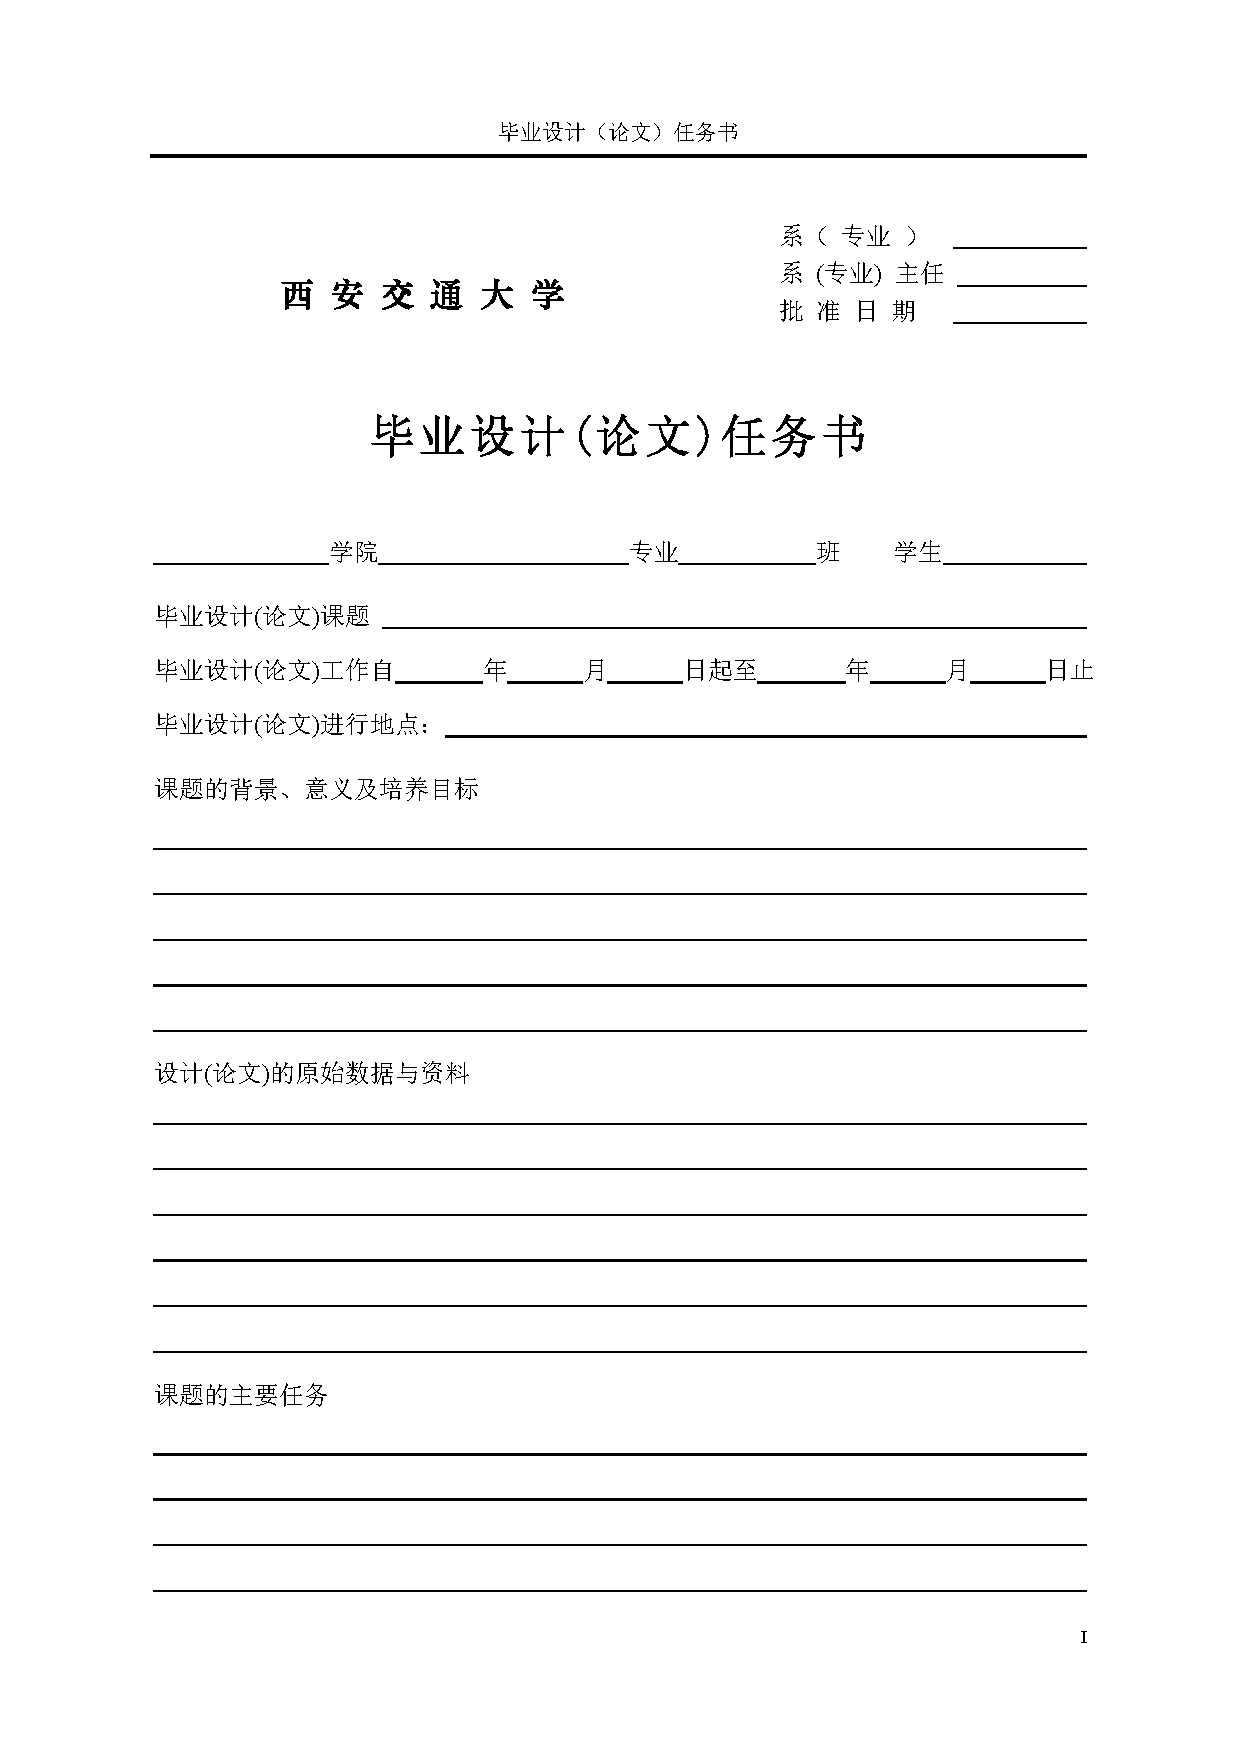
\includepdf[pages=-]{pdfs/任务书.pdf}
% 
\includepdf[]{pdfs/考核评议书.pdf}
% 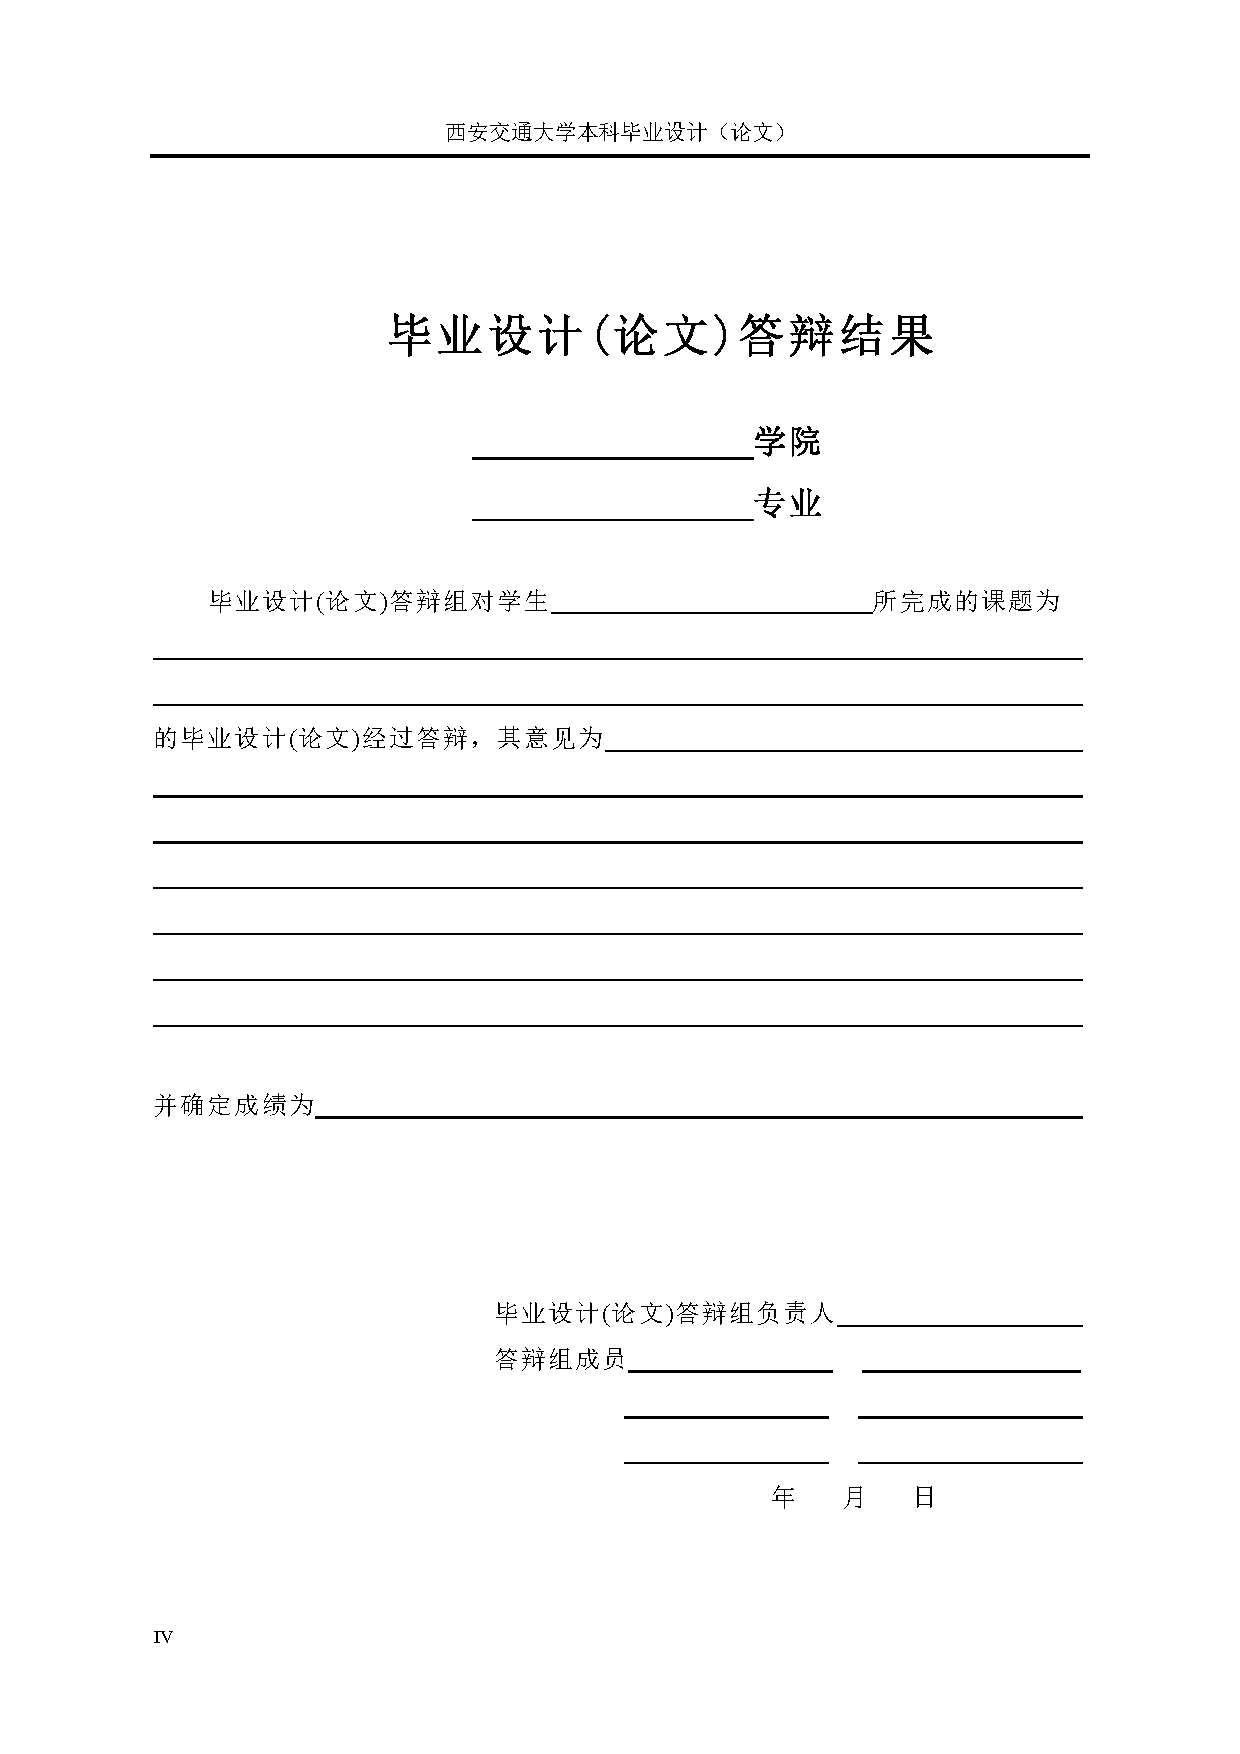
\includepdf[]{pdfs/答辩结果.pdf}


% !Mode:: "TeX:UTF-8" 

%-----------------------------------------------------------------------------------------
% 中文摘要
\clearpage
\titlespacing{\chapter}{0pt}{0mm}{5mm}
% \Abstract{摘\quad 要}{Abstract (In Chinese)}
\BiAppendixChapter{摘\quad 要}{Abstract (In Chinese)}
% \chapter{摘\quad 要}

\defaultfont
本文提出了一种基于非嵌入式离线强化学习的训练策略,通过图像信息输入在即时策略游戏皇室战争(Clash Royale)中实现自主博弈对局。
本文结合当前目标识别与光学文本识别的前沿算法对图像信息进行特征提取,并使用离线强化学习算法进行训练,
实现了移动设备上的实时图像获取、图像感知特征融合、智能体决策及设备控制,与对手进行实时对局,并能够战胜游戏中的内置AI。

首先,本文设计了一种高效制作切片数据集的方法,在此基础上制作了包含$4654$张切片的数据集,涵盖了游戏中的全部部队、法术、防御塔等总计$150$个类别。
本文提出了一种生成目标识别数据集的算法,能够模拟真实对局场景生成带标签图像,用于目标识别模型训练。
本文从视频流中截取$6939$张图像,制作了包含$116878$个目标框的目标识别数据集作为验证集\footnote{图像数据集:\url{https://github.com/wty-yy/Clash-Royale-Detection-Dataset}\hfill}。
通过生成式数据集训练出的目标识别模型在验证集中表现出良好的泛化性,在$50\%$交并比阈值下达到了$80.9\%$的召回率。

其次,基于目标识别、光学文本识别及图像分类模型的输出特征,本文设计了图像感知融合算法,能够将感知特征预处理为模型的输入特征。
该算法基于视频数据中的上下帧信息及单位的关联信息恢复漏识别目标,
排除干扰性特征,优化模型输入特征。

最后,在决策模型方面,本文制作了包含$105$个回合、总共$113981$帧的专家数据集\footnote{专家数据集:\url{https://github.com/wty-yy/Clash-Royale-Replay-Dataset}\hfill},
在智能体不与环境交互的条件下进行训练。本文从架构及预测目标两个方面对离线强化学习模型进行了改进,将难以学习的离散动作序列转化为连续动作序列,
相比传统模型性能分别提高了$24\%$和$37\%$。

本文的全部代码均已开源\footnote{全部代码:\url{https://github.com/wty-yy/katacr}}。

\vspace{\baselineskip}
% \noindent{\textbf{关键词:}} 非嵌入式游戏AI;生成式目标识别数据集;离线强化学习
\noindent{\textbf{关键词:}} 目标识别;光学文本识别;强化学习

%-----------------------------------------------------------------------------------------
% 英文摘要
\clearpage
%\phantomsection
\setcounter{footnote}{0}
\markboth{Abstract}{Abstract}

\titlespacing{\chapter}{0pt}{0mm}{5mm}
% \chapter*{ABSTRACT}
\BiAppendixChapter{ABSTRACT}{}
% \chapter{Abstract}

\noindent This thesis proposes a training strategy based on non-embedded offline reinforcement learning to achieve autonomous gameplay in the real-time strategy game Clash Royale through image information input.
The thesis integrates cutting-edge algorithms for object recognition and optical character recognition to extract features from image information and uses offline reinforcement learning algorithms for training.
This enables real-time image acquisition, perception fusion, agent decision-making, and device control on mobile devices, allowing real-time matches against opponents and defeating the built-in AI in the game.

\noindent Firstly, the thesis designs an efficient method for creating a sliced dataset and produces a dataset containing 4654 slices, covering all troops, spells, and towers in the game, totaling 150 categories. The thesis proposes an algorithm to generate an object recognition dataset that can simulate real-game scenarios to
generate labeled images for training object recognition models. The thesis extracts 6939 images from video streams, creating an object recognition validation dataset containing 116878 bounding boxes\footnote{Image dataset: \url{https://github.com/wty-yy/Clash-Royale-Detection-Dataset}\hfill}. The object recognition model trained with the generative dataset shows good generalization in the validation set, achieving an 80.9\% recall rate at a 50\% Intersection over Union (IoU) threshold.

\noindent Secondly, based on the output features of object recognition, optical character recognition, and image classification models, the thesis designs a perception fusion algorithm that preprocesses perception features into model input features. The algorithm recovers missed targets based on inter-frame information and unit association information in the video data, eliminating interfering features and optimizing the model input features.

\noindent Finally, in terms of the decision-making model, the thesis creates an expert dataset containing 105 rounds and a total of 113981 frames\footnote{Expert dataset: \url{https://github.com/wty-yy/Clash-Royale-Replay-Dataset}\hfill}, training the agent without interacting with the environment. The thesis improves traditional offline reinforcement learning models from both architecture and prediction objectives, transforming hard-to-learn discrete action sequences into continuous action sequences, improving performance by 24\% and 37\% compared to traditional models, respectively.

\noindent All code in this thesis has been open-sourced\footnote{All code: \url{https://github.com/wty-yy/katacr}}.

\vspace{\baselineskip}
\noindent{\textbf{Keywords:}} Object recognition; Optical character recognition; Reinforcement learning
% \noindent{\textbf{Keywords:}} Non-embedded game AI; Generative object detection dataset; Offline reinforcement learning


\titlespacing{\chapter}{0pt}{-6mm}{5mm}
\clearpage{\pagestyle{empty}\cleardoublepage}
  % 摘要
% !Mode:: "TeX:UTF-8" 

% 中文目录
\defaultfont
\pdfbookmark[0]{目~~~~录}{mulu}
\tableofcontents
\clearpage{\pagestyle{empty}\cleardoublepage}

% 英文目录
% \pdfbookmark[0]{Contents}{econtent}
% \tableofengcontents
% \clearpage{\pagestyle{empty}\cleardoublepage}
  % 目录
\clearpage


\titlespacing{\chapter}{0pt}{0mm}{5mm}
\BiAppendixChapter{主要符号表}{denotation}
\defaultfont

% \printnomenclature

% \nomenclature{$\displaystyle a$}{The number of angels per unit are}
% \nomenclature{$\displaystyle N$}{The number of angels per needle point}
% \nomenclature{$\displaystyle A$}{The area of the needle point}
% \nomenclature{$\displaystyle \sigma$}{The total mass of angels per unit area}
% \nomenclature{$\displaystyle m$}{The mass of one angel}
% \nomenclature{$\displaystyle \sum_{i=1}^n a_i$}{The sum of $a_i$}

\begin{labeling}{~~~~~~~~~~~~~~~~~~~~~}
\setlength{\parskip}{0pt plus1pt minus1pt}
\item [$\mathbb{R}$] 实数集
\item [$\mathbb{N}$] 自然数集
\item [$\mathbb{Z}$] 整数集
\item [$\mathbb{Z}^+$] 正整数集
\item [$\mathbb{R}^N$] $N$维空间,由$N$个实数集$\mathbb{R}$所构成的笛卡尔积
\item [$\text{[条件]}$] 当“条件”成立时为$1$,否则为$0$
\item [$A_{ij}$] 矩阵$A$的第$i$行第$j$列元素
\item [$\bd{x}_i$] 向量$\bd{x}$中第$i$个元素
\item [$\bd{x}_{i:j}$] 向量$\bd{x}$中第$i$到$j$个元素所构成的向量
\item [$\text{softmax}(\bd{z})$] $\displaystyle\left\{\frac{\e^{z_i}}{\sum_{j=1}^Ce^{z_j}}\right\}_{i=1}^C$其中向量$\bd{z}\in\mathbb{R}^{C}$,$C$为总类别数
\item [$A\odot B$] $(A\odot B)_{ij} = (A)_{ij}(B)_{ij}$其中矩阵$A$与矩阵$B$具有相同形状

\end{labeling}
\titlespacing{\chapter}{0pt}{-6mm}{5mm}
%\clearpage{\pagestyle{empty}\cleardoublepage}
\let\cleardoublepage\clearpage  % 消除空白页
  % 符号解释

%======================================= Main Body =======================================
\mainmatter\defaultfont\sloppy\raggedbottom

% !Mode:: "TeX:UTF-8" 

\BiChapter{绪论}{xu lun}
\BiSection{嵌入式智能体研究现状}{xu lun 1}
当前强化学习(Reinforcement Learning, RL)已经成为人工领域备受关注的重点之一,
它通过智能体与环境交互利用得到的奖励大小来指导策略的改进,
通过不断地试错来获得最优策略。

强化学习在游戏领域中有着广泛的应用:围棋作为经典博弈游戏,
因其具有巨大的状态空间以及复杂的策略而无法使用传统搜索算法解决,
DeepMind团队通过AlphaGo\upcite{AlphaGo}给出了基于价值函数估计和蒙特卡洛树搜索的解决方法,
首次打败人类顶级选手,标志着强化学习在处理复杂游戏中的巨大成功;
AlphaZero\upcite{AlphaZero}也使用类似模型架构,但它完全基于自我博弈学习,
在摒弃任何人类先验知识的前提下超越了AlphaGo,它展现了自博弈学习的强大能力。

多人在线战术竞技游戏中强化学习也有着非凡的成就,这类游戏往往有着巨大的动作、状态空间,
并带有高动态的前后文信息,需要智能体之间的团队配合能力。
OpenAI公司通过OpenAI Five\upcite{OpenAIFive}给出了基于强化学习的解决方法,
该深度网络模型为长短期记忆循环神经网络(Long Short-Term Memory,LSTM)\upcite{LSTM}和卷积神经网络(Convolutional Neural Network, CNN)组合,
提出并利用了强化学习中经典在线同策略近端策略优化算法
(Proximal Policy Optimization, PPO)算法\upcite{PPO},
使用分布式训练方法使其首次在Dota2游戏中战胜顶级职业选手。
类似的还有DeepMind团队的AlphaStar\upcite{AlphaStar}在即时战略游戏《星际争霸》中解决了复杂的多智能体决策问题。

% 在即时战略游戏(Real-Time Strategy,RTS)中,星际争霸(StarCraft)作为经典游戏,其需要玩家同时控制数百个智能体进行团队配合,
% 并需要对各类资源进行合理分配。DeepMind团队通过AlphaStar\upcite{AlphaStar}给出了基于自博弈、
% 多智能体强化学习的算法,模型采用CNN和注意力机制(Attention)处理时空信息,该模型同样超越顶级职业选手。

值得注意的是上述模型使用的算法均为在线强化学习算法即经典强化学习研究内容,
经典算法例如PPO\upcite{PPO}、深度Q函数学习(Deep Q Network, DQN)\upcite{DQN}、软演员评论家算法(Soft Actor-Critic, SAC)等,
这是因为嵌入式智能体与游戏环境之间本身具有低成本高交互次数的特性,使得智能体有无限的试错空间,可以不断对新状态空间进行探索,
更好地对动作状态价值函数$Q(s,a)$进行估计,
并进一步利用$Q(s,a)$对自身策略$\pi(a|s)$进行优化,从而通过迭代方法接近最优策略$\pi^*(a|s)$。

由于嵌入式智能体对环境信息的读取和人类完全不同,人类理解视频游戏的主要方式是通过图像信息,
而嵌入式智能体可以直接获取精确的游戏内部信息,虽然这些人类也可以通过图像信息间接获得,
但可视化的图像信息中往往伴有噪声,在信息输入方面就会产生误差,因此就导致了游戏竞技上的不公平性产生
(其余的不公平因素,例如感知频率与操作频率,对智能加入相应限制可以解决)。

由于当前计算机视觉技术(Computer Vision, CV)发展迅速,本论文提出一种非嵌入智能体的特征提取方法,
这种非嵌入式智能体可以仅通过获取和人类完全相同的图像信息进行决策,
由于非嵌入式智能体只能通过模拟器和环境进行交互,无法高效获取数据,
所以本文只能收集专家数据集,采用~\ref{sec-offline-rl}~中所介绍的离线强化学习算法Decision Transformer(DT)\upcite{DT}
和StARformer\upcite{StARformer}来完成决策部分。

\BiSection{计算机视觉研究现状}{xu lun 2}
非嵌入式智能体主要利用到计算机视觉中图像分类(Image Classfication)、目标识别(Object Detection)和
光学字符识别(Optical Character Recognition, OCR)三个方面,下面分别对其进行简单介绍:
% \BiSubsection{图像分类}{xu lun 3}
\paragraph*{图像分类}在图像分类任务上LeNet-5\upcite{LeNet}给出了早期卷积神经网络(Convolutional Neural Network, CNN)模型,它作为现在CNN架构的先驱之一,
在MNIST手写数据集上首次展现出深度神经网络的卓越性能。近年来由于自动微分计算速度的飞速提升以及ImageNet2012数据集\upcite{ImageNet}的支撑,
从而使得基于数据驱动的模型重新被重视,自从AlexNet\upcite{AlexNet}利用在2012年ImageNet挑战赛中取得突破性成果后,
各类新型网络架构例如VGG\upcite{VGG}、GoogleNet\upcite{GoogleNet}、ResNet\upcite{ResNet}、DenseNet\upcite{DenseNet}、
ViT\upcite{ViT}、RepVGG\upcite{RepVGG}、MetaFormer\upcite{MetaFormer}等相继被提出,这些模型不断刷新图像分类的准确率记录,同时提升了模型的计算能力和泛化能力。

研究者针对网络的宽深度(VGG)、宽度(GoogleNet)、残差连接(ResNet)、分组卷积(AlexNet)、注意力机制(ViT, MetaFormer)、模型重新参数化(RepVGG)等方面进行了深入探索,
其中残差网络的引入解决了深度网络的训练难题,可以将网络深度上升到数百层之上,乃至Transformer\upcite{transformer}类架构中也使用了残差机制;
而注意力机制的引入可以帮助模型关注图像的关键特征。
% \BiSubsection{目标识别}{xu lun 4}
\paragraph*{目标识别}
目标识别任务(Object Detection)旨在从图像或视频数据中识别出特征类别的目标或对象,
根据处理流程的不同检测头(Detection Head)分为单阶段检测器(Single-Stage Detectors)和多阶段检测器(Two-Stage Detectors),
其中单阶段检测器,通常为端到端问题,直接通过输入的图像给出识别框的位置(回归问题)与类别(分类问题),
当前经典模型包括YOLO(You Only Look Once)v1~$\sim$~9系列\upcite{YOLO}、
SSD(Single Shot Multibox Detector)\upcite{SSD}、DETR(DEtection TRansformer)\upcite{DETR}等。
这类算法优点在与推理速度较快,适用于实时监测任务,该系列在初次提出时检测率较低,但通过不断的优化改进,已经可以成功的解决小目标检测和重叠目标问题。
而多阶段检测器例如R-CNN\upcite{FastRCNN}系列,这类算法虽精度较高,但推理速度较长,不适用于实时监测任务。
% \begin{itemize}[left=2ex]
%   \item 单阶段检测器(Single-Stage Detectors),通常为端到端问题,直接通过输入的图像给出识别框的位置(回归问题)与类别(分类问题),
%   当前经典模型包括YOLO(You Only Look Once)v1~$\sim$~9系列\upcite{YOLO}、
%   SSD(Single Shot Multibox Detector)\upcite{SSD}、DETR(DEtection TRansformer)\upcite{DETR}等。
%   这类算法优点在与推理速度较快,适用于实时监测任务,该系列在初次提出时检测率较低,但通过不断的优化改进,已经可以比较成功的解决小目标检测和重叠目标任务。
%   \item 多阶段检测器(Two-Stage Detectors),通常将检测过程分为两个阶段,首先生成候选区域(Region Proposals),
%   然后再对候选区域进行分类和精确定位,经典的多阶段如R-CNN\upcite{FastRCNN}系列。但这类算法由于推理速度较长,不适用于实时监测任务。
% \end{itemize}
% \BiSubsection{光学字符识别}{xu lun 5} 
\paragraph*{光学字符识别}
光学字符识别(OCR, Optical Character Recognition)目前最常用的模型是卷积循环神经网络(Convolutional Recurrent Neural Networks, CRNN)\upcite{CRNN},
其将经典的连接时序分类损失函数(CTC,Connectionist Temporal Classification)\upcite{CTC}与深度神经网络架构LSTM和CNN相结合,
首先利用CNN将图像信息编码为一维序列信息,再用(Bi-)LSTM\upcite{BiLSTM}进行文本预测,最后利用CTC损失函数使用对预测的文本顺序进行纠正。
但是仅有文字识别模型并不足够,还需要对图像中的文本位置进行定位再使用CRNN算法进行识别,
于是发展出了很多OCR系统,如百度公司的PP-OCRv1~$\sim$~4系列\upcite{PPOCR}。

为了理解每个模型的搭建与训练细节,本文对上述介绍的部分模型进行了复现\footnote{\url{https://github.com/wty-yy/katacv},复现内容包括:LeNet-5、AlexNet、VGG16、GoogleNet、ResNet50、
YOLOv1、YOLOv3、YOLOv4、YOLOv5、CTCLoss \& CRNN、miniGPT}。

\BiSection{本毕设的任务}{xu lun 6}
\begin{wrapfigure}[26]{r}{.5\textwidth} % 文字环绕行数为13行, 图片靠右 (l为靠左), 图片占0.3的行宽
  \vspace{-4ex}\centering
  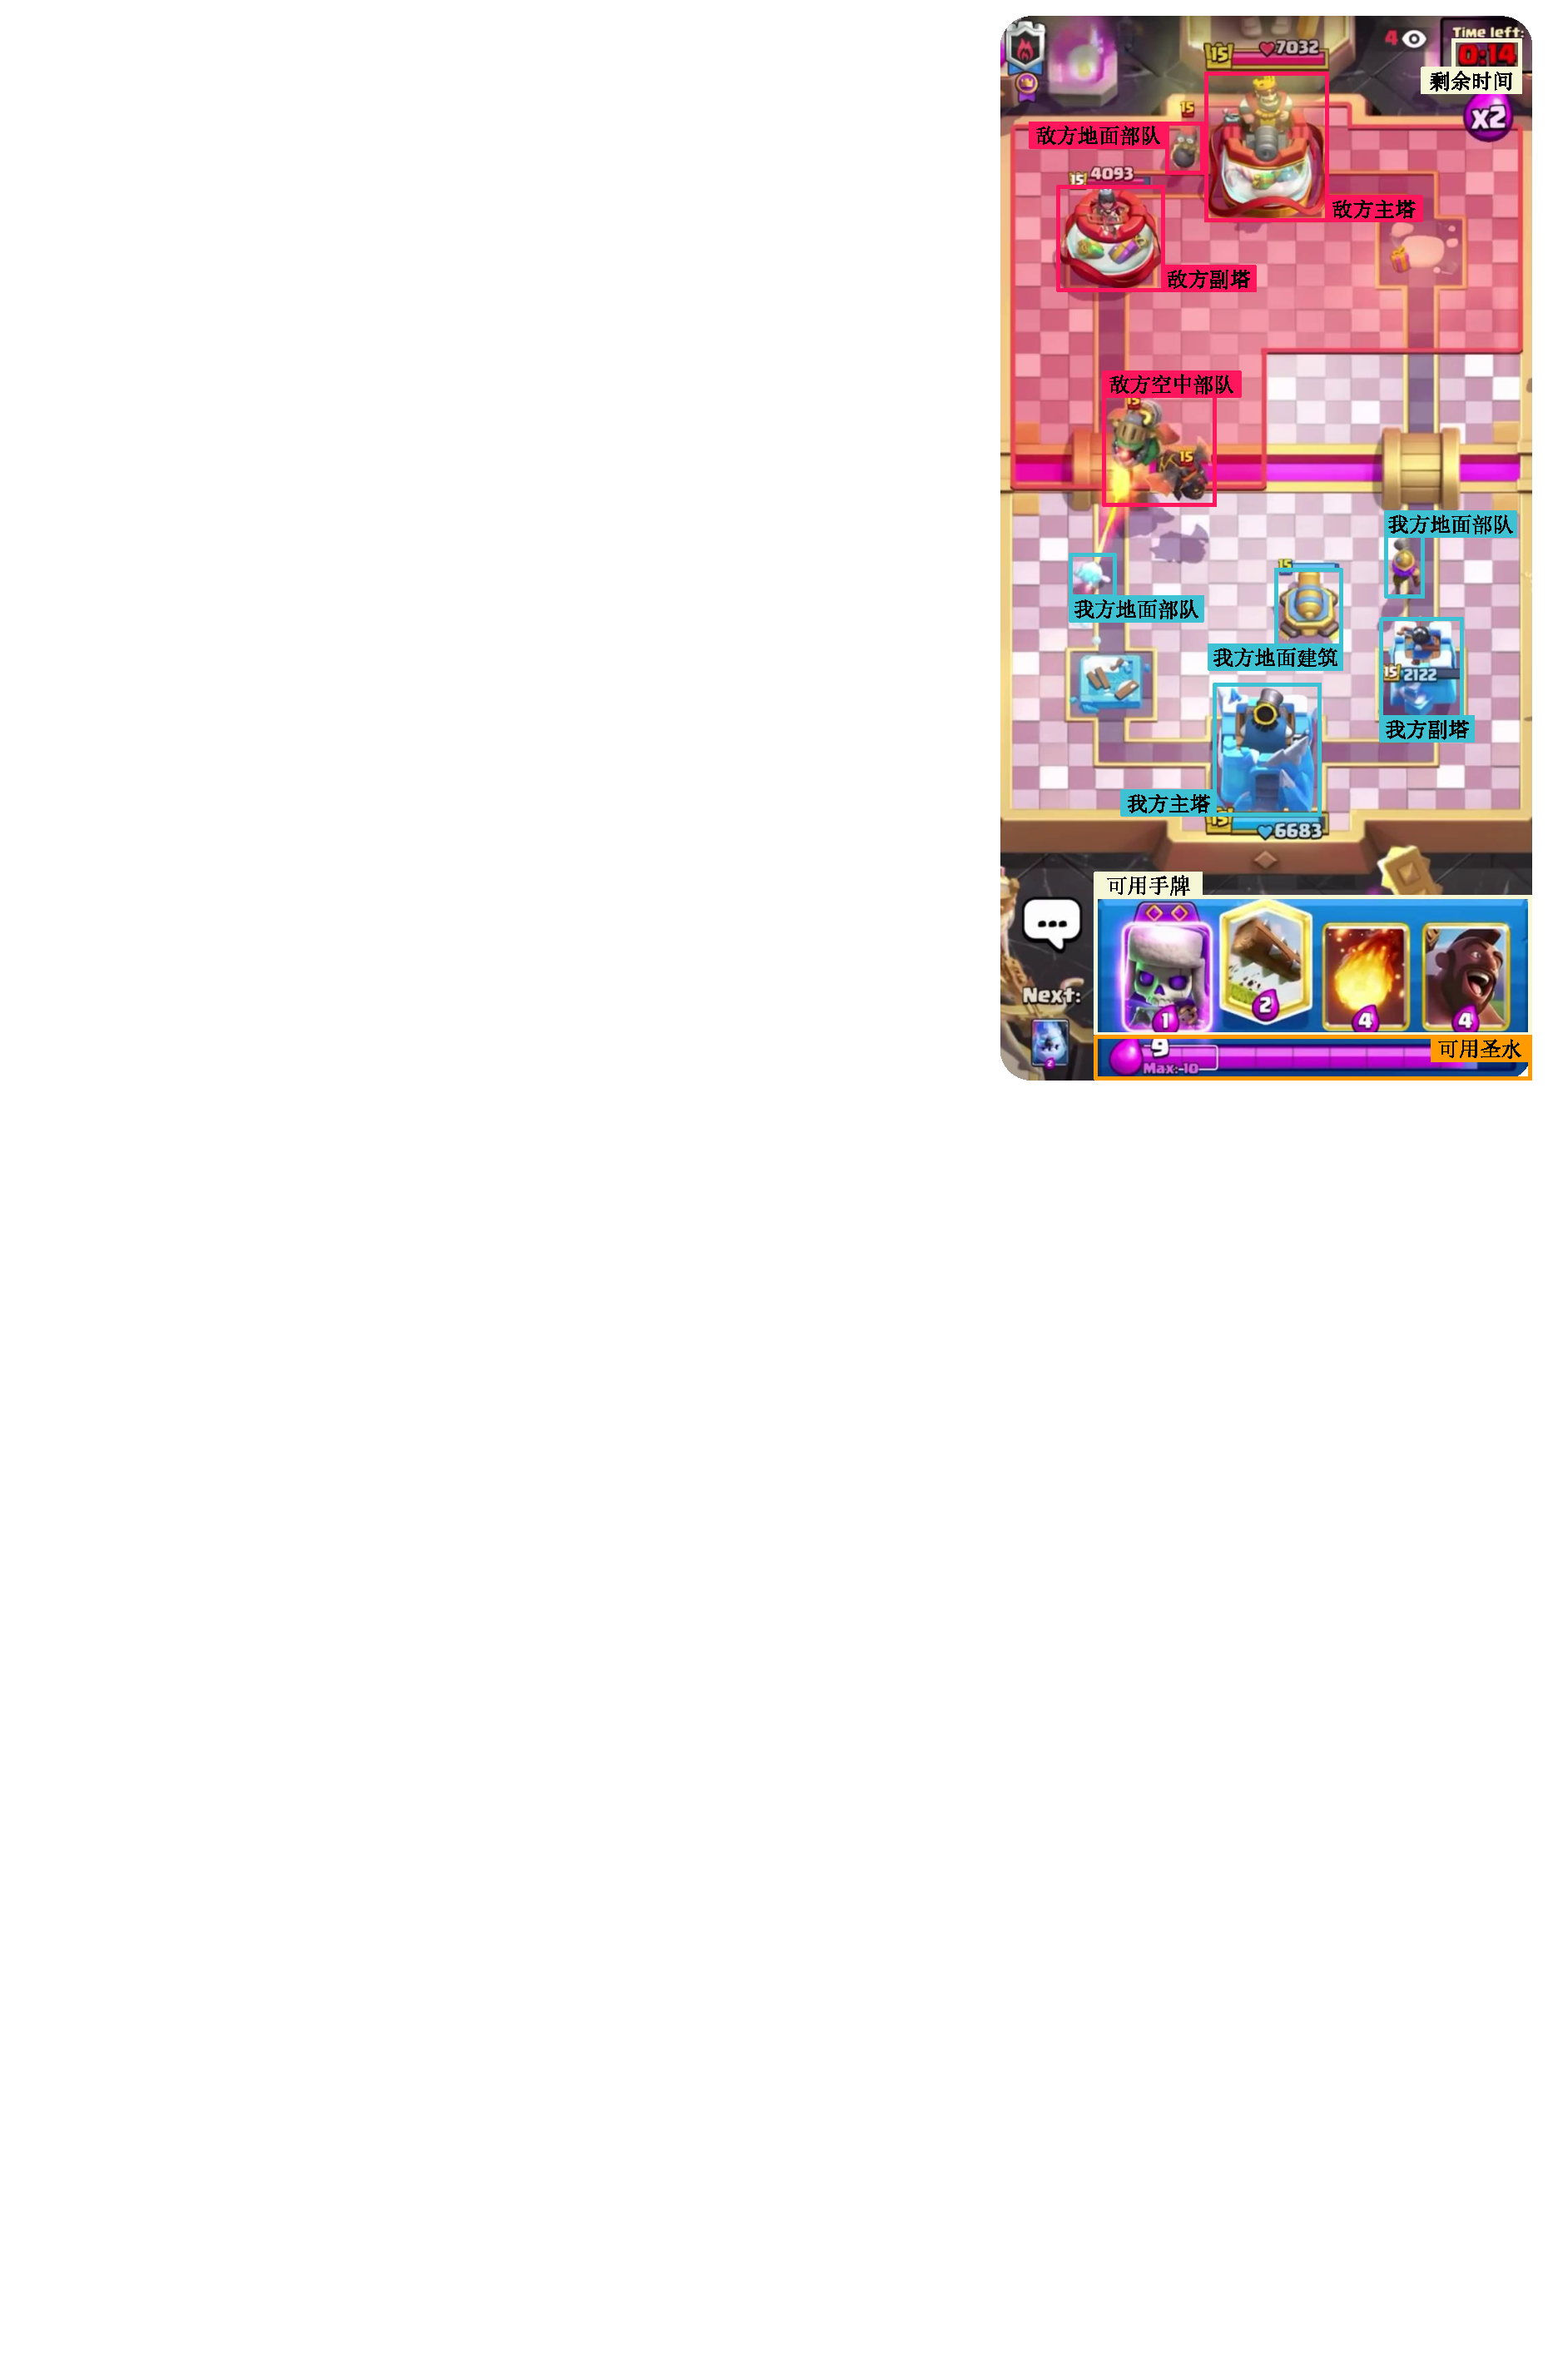
\includegraphics[width=0.5\textwidth]{introduction.pdf}
  \caption{右上角为当前阶段的剩余时间;中间为竞技场部分,双方可在其上部署部队及建筑;
  下方显示了可用手牌以及部署所需的圣水,最下方显示了当前的可用圣水总量。}
  \label{fig-introduction}
\end{wrapfigure}
《皇室战争》(Clash Royale, CR)是一款卡牌类即时策略游戏(RTS),本文仅考虑一对一对战模式,
双方玩家需要通过实时决策使用手牌来战胜对手,首先对游戏基本规则及非嵌入式感知任务目标进行介绍:
\paragraph*{感知场景}在对局过程中,游戏场景如右图~\ref{fig-introduction}~所示,本文所需的感知内容主要分为如下四个主要部分和三个子部分:

\noindent 主要部分:
\begin{itemize}[left=1em]
  \item 竞技场(Arena):包括防御塔及双方所部署的部队和建筑物。
  \item 手牌:位于竞技场下方,包括当前卡片图像及其所需的圣水(Elixir)。
  \item 游戏时间:当前阶段的剩余时间。
  \item 总圣水:用于卡牌的使用,随时间自动恢复。
\end{itemize}

\noindent 子部分:
\begin{itemize}[left=1em]
  \item 主塔:处于三个防御塔中间,当其被摧毁时,对局直接结束。
  \item 副塔:处于左右两侧的防御塔。
  \item 部队:玩家通过卡牌部署的战斗单位,包括可移动地面和空中单位,以及建筑单位。
\end{itemize}

% 这里一定要空一行
\paragraph*{游戏目标}每位玩家的目标是摧毁尽可能多的敌方防御塔,优先摧毁敌方主塔的玩家立刻获胜。
游戏中在两种阶段下存在不同的胜利条件:\label{game-target}
\begin{enumerate}
  \item 常规时间:持续三分钟,目标为摧毁更多的敌方防御塔,若时间结束时防御塔数量一致,则进入加时赛,
  否则防御塔多的一方获胜。
  \item 加时赛:持续两分钟,在该阶段中,首个摧毁敌方剩余防御塔的玩家获胜,
  若加时赛结束时仍未分出胜负,则比较双方防御塔的最低生命值,最低生命值较高者获胜,若仍未分出胜负,则为平局。
\end{enumerate}
\paragraph*{游戏过程}一次对局中每个玩家牌库大小为固定的8张,对局开始时,随机在队列中初始化卡牌的出现顺序,
每次从队首取出4张手牌,当玩家使用卡牌后,使用完的卡牌将被重新加入队尾,
所以当一方使用完8张不同卡牌时,可以通过逻辑计算出未出现卡牌类别。
玩家需要基于当前竞技场上的实时状态、手牌类别及总圣水信息,
实时决策使用卡牌的类别和位置,采取进攻或防守策略,最终按照上述给出的规则自动判断胜负。

\BiSection{本毕设的贡献}{xu lun 7}
\begin{figure}[htbp]
  \centering\vspace{-3ex}
  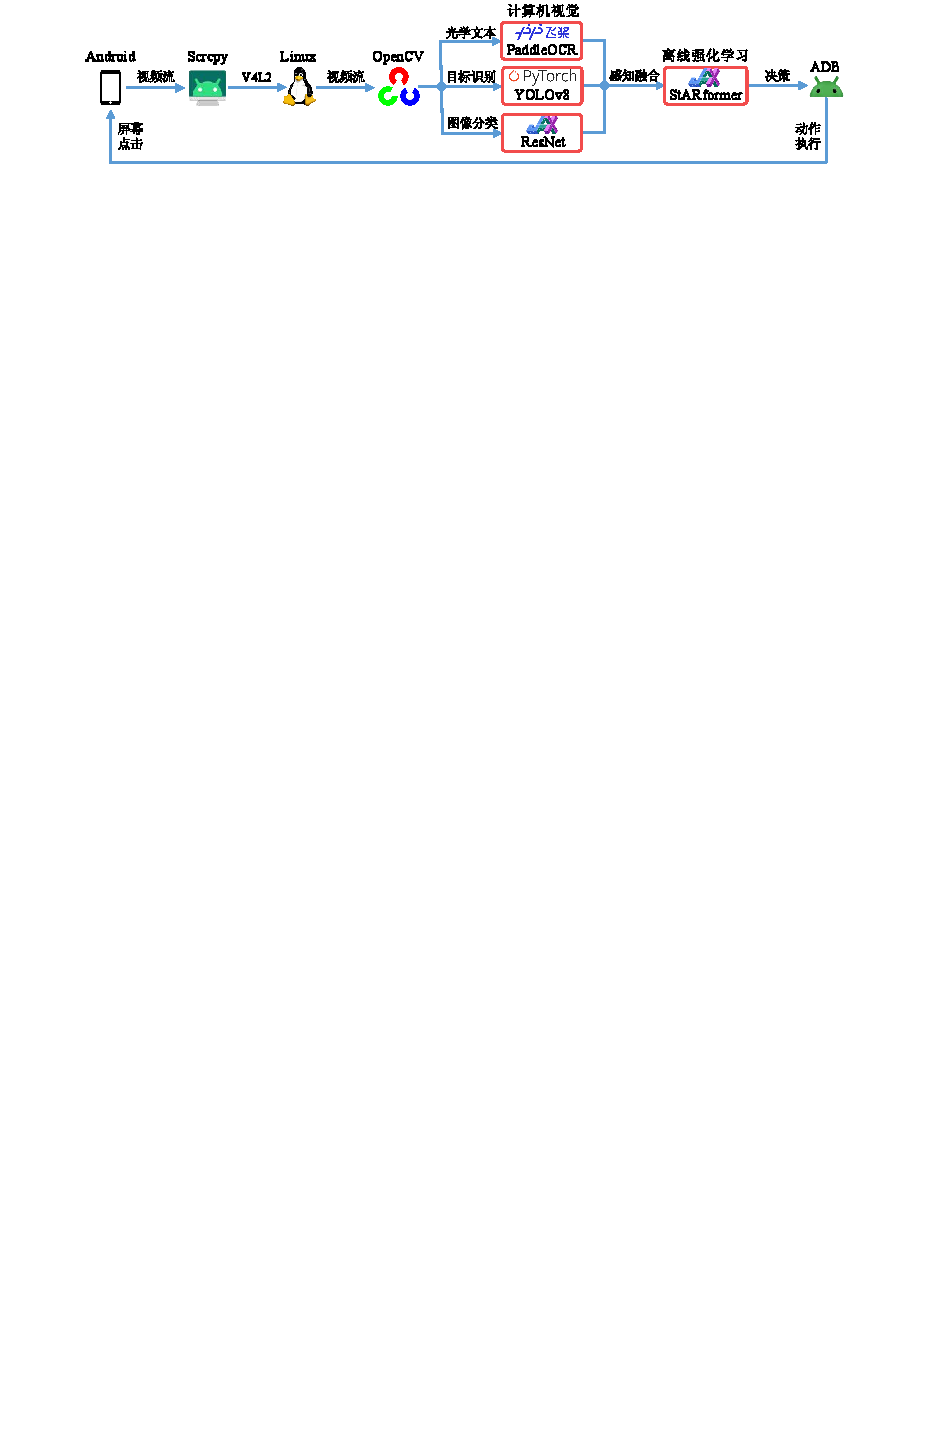
\includegraphics[width=\textwidth]{framework.pdf}
  \caption{信息流传输流程图}\label{fig-framework}
\end{figure}
在本文中,首次提出一种基于非嵌入式的离线强化学习设计方案,应用于游戏《皇室战争》,
并最终在移动端设备上进行实时决策验证其可行性。图~\ref{fig-framework}~中展示了信息流的传输流程,其中感知与决策模型的设计方案如下:
\begin{enumerate}
  \item 生成式数据集:本文设计了一个与本任务相关的生成式数据集,使其可以模仿真实场景生成含有任意数量部队及种类的带有识别标签的图像,
  能够非常高效地生成用于目标识别的训练数据集。
  \item 感知融合:本文利用YOLOv8\upcite{YOLOv8}并结合目标追踪技术ByteTrack\upcite{ByteTrack}实现了对视频流中部队位置及类别的实时识别,
  通过PaddleOCR\upcite{PPOCR}完成了对数字及时间信息的识别,利用ResNet\upcite{ResNet}完成对卡牌和圣水图标的分类,
  结合上述几种感知模型,本文还提出了一系列针对于本任务的上下帧信息过滤方法用于优化感知特征。
  \item 模型决策:本文使用离线强化学习算法StARformer作为决策模型,
  设计相应的特征输入结构以及损失函数,并将难以学习的离散动作序列转化为连续动作序列进行训练,
  此方法大幅提高模型性能,最后部署在手机上完成实时对局决策。
\end{enumerate}

离线强化学习模型使用手工录制的11万帧专家数据集进行训练,
能够战胜游戏内置AI,虽然无法达到$100\%$胜率,但本研究发现该离线强化学习模型能够展现出一定的模仿及泛化能力,
从一定程度上说明了这种非嵌入式方法的可行性。

图~\ref{fig-eval-display}~中展示了电脑对手机的实时控制效果。图~\ref{fig-eval-computer-vid}~中具体内容如下:
左一为手机视频流;
左二为感知识别结果,左上角为当前实时奖励与总帧数,右上角为当前回合经过的时间,左下角为当前总圣水与手牌,竞技场中目标识别的边界框名称中第一项为类别名称与从属派别,第二项为目标跟踪编号;
右二为感知融合特征,其中网格为$32\times 18$与竞技场中的格子相对应,每个带颜色的方形表示一个部队(数字表示从属派别),圆形表示观测到的动作执行(左上数字为卡牌编号,右下角为动作滞后的帧数);
右一为StARformer-3L决策模型的实时预测的动作分布,其中上方的网格分布表示动作的二维坐标预测,左下角数字表示当前预测动作延迟帧数,右下角四个方格对应四张手牌被选的概率大小。

\begin{figure}[h!]
  \centering\vspace{-1ex}
  \subfigure[现实场景:左侧为被控制的手机,右侧为电脑\label{fig-eval-real}]{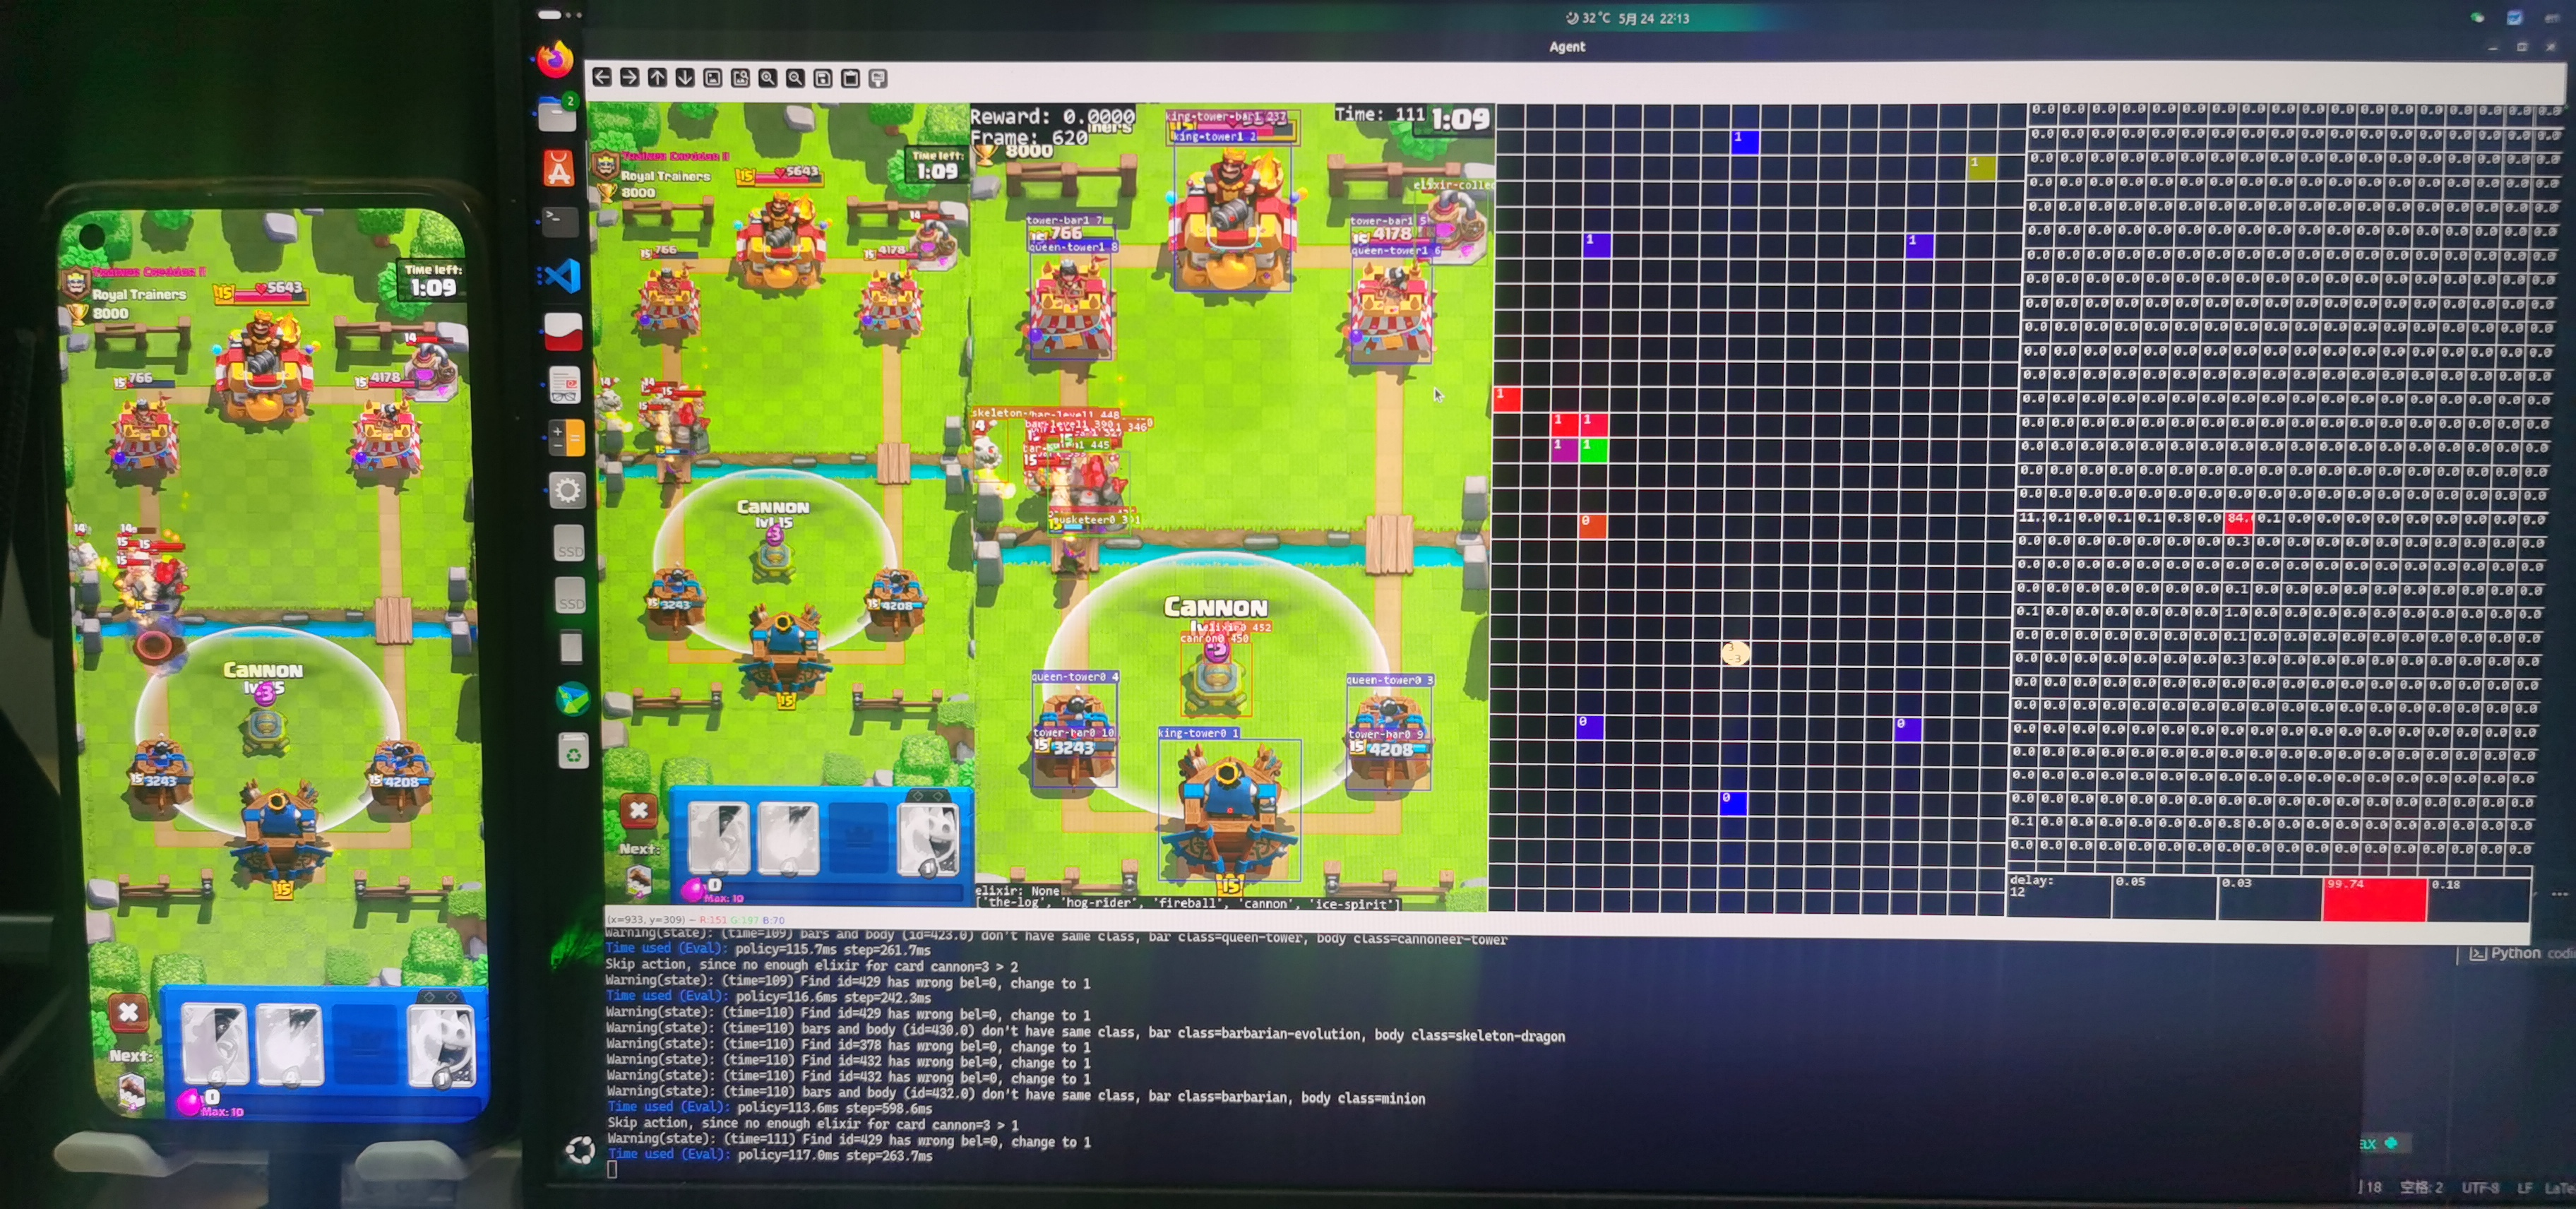
\includegraphics[width=\textwidth]{eval_online_real.jpg}}
  \subfigure[电脑中感知融合与决策:左一为手机视频流,左二为感知识别结果,右二为感知融合特征,右一为模型决策预测动作分布。
  \label{fig-eval-computer-vid}]{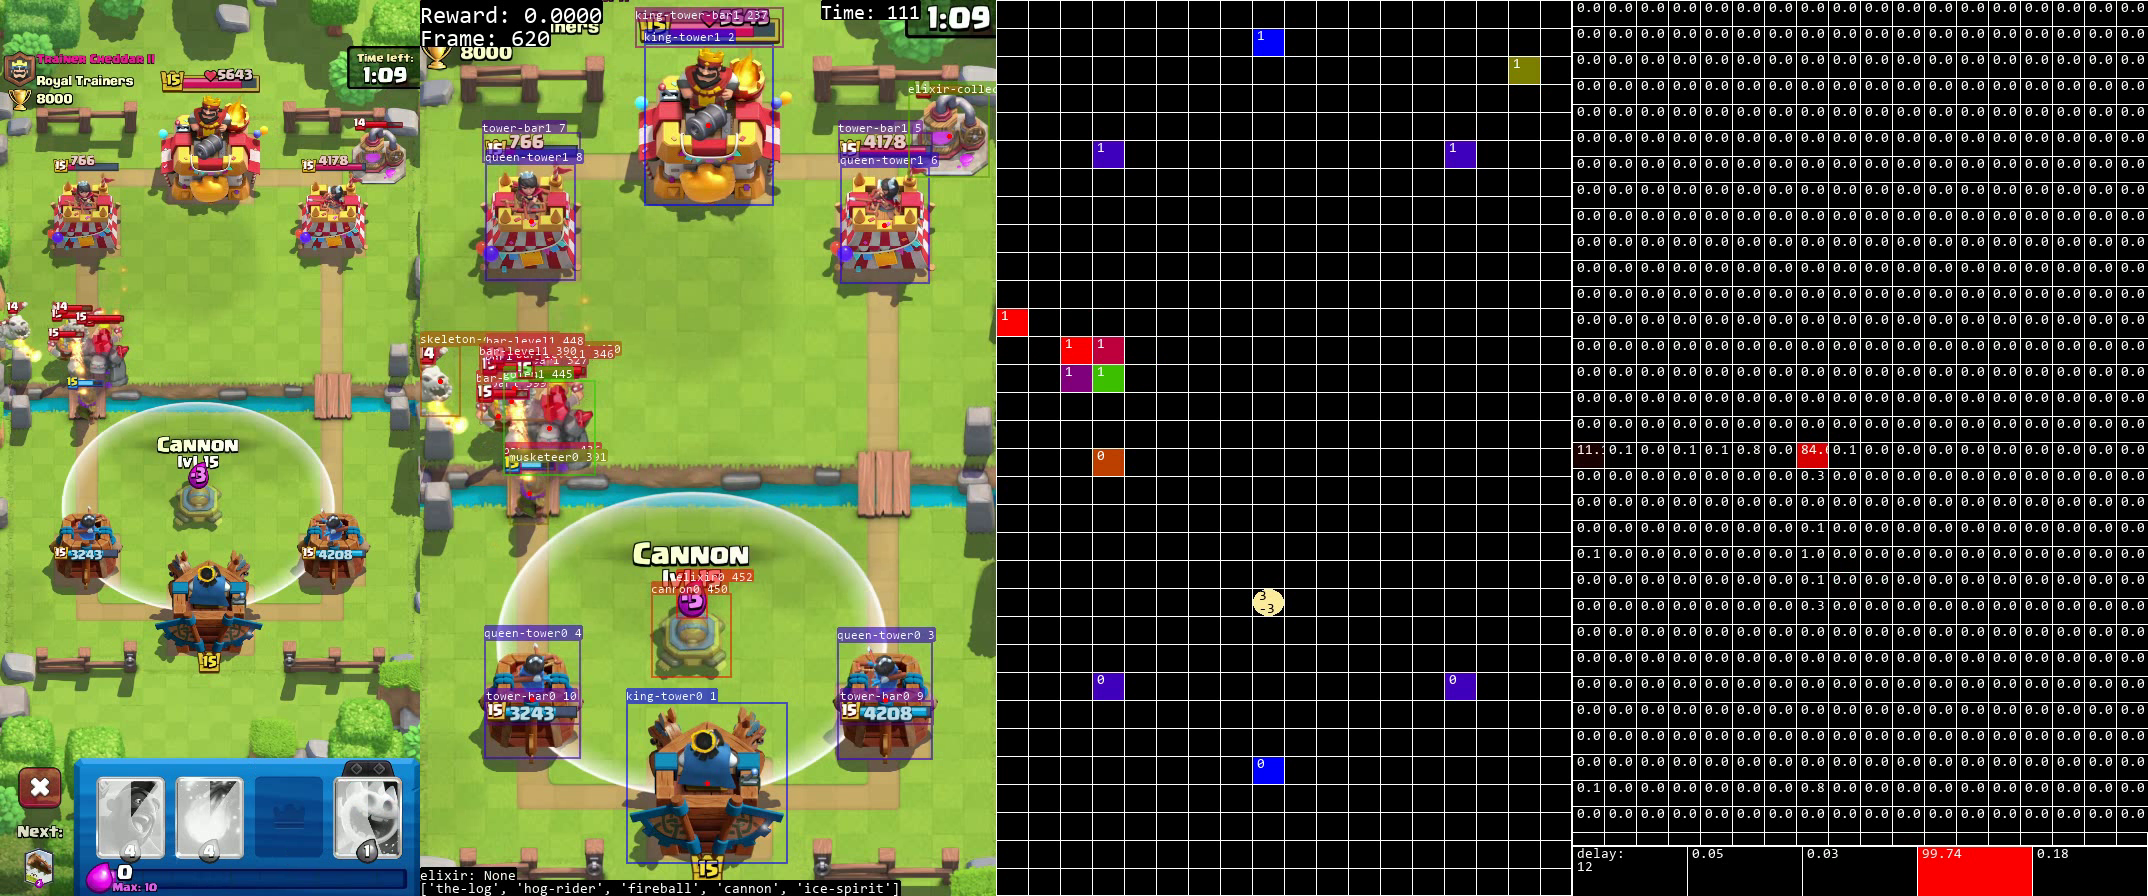
\includegraphics[width=\textwidth]{eval_online_vid.png}}
  \setlength{\abovecaptionskip}{0ex}  % 由于minted会增大图像与标题间距需要进行缩小
  \vspace{-1ex}
  \caption{实时控制效果}
  \label{fig-eval-display}
\end{figure}
  % 正文
% !Mode:: "TeX:UTF-8" 

\BiChapter{目标识别数据集搭建及模型架构设计}{2}
本毕设的首要任务是完成图~\ref{fig-introduction}~中竞技场部分的目标识别问题,
因为决策所需的状态信息主要来自于该部分,对于竞技场中第$i$各单位$u_i$,
其所包含的信息可以表示为$u=(\boldsymbol{x}, \text{cls}, \text{bel}, \text{bar}_1, \text{bar}_2)$,
其中$\boldsymbol{x}$表示$u$所在的网格坐标,$\text{cls}$表示$u$所属的部队类别,
$\text{bel}$表示$u$所属的派别,$\text{bar}_1,\text{bar}_2$表示$u$当前的生命值及其余条状图像信息。

在本章节将介绍如何使用目标识别模型完成对每个单位中$\boldsymbol{x}, \text{cls}, \text{bel}$信息的识别,
由于训练目标识别模型需要基于大量的有标记图像,而该任务没有任何相关的开源数据集,若逐帧人工标记效率极低且成本高昂,
因此本毕设基于该任务提出一种高效的带标记图像的生成方案,并目标识别代码使其可以有效训练该生成式数据集以满足上述识别要求,
识别数据集制作以及模型更新流程如图~\ref{fig-annotation}~所示。
\begin{figure}[htbp]
  \centering
  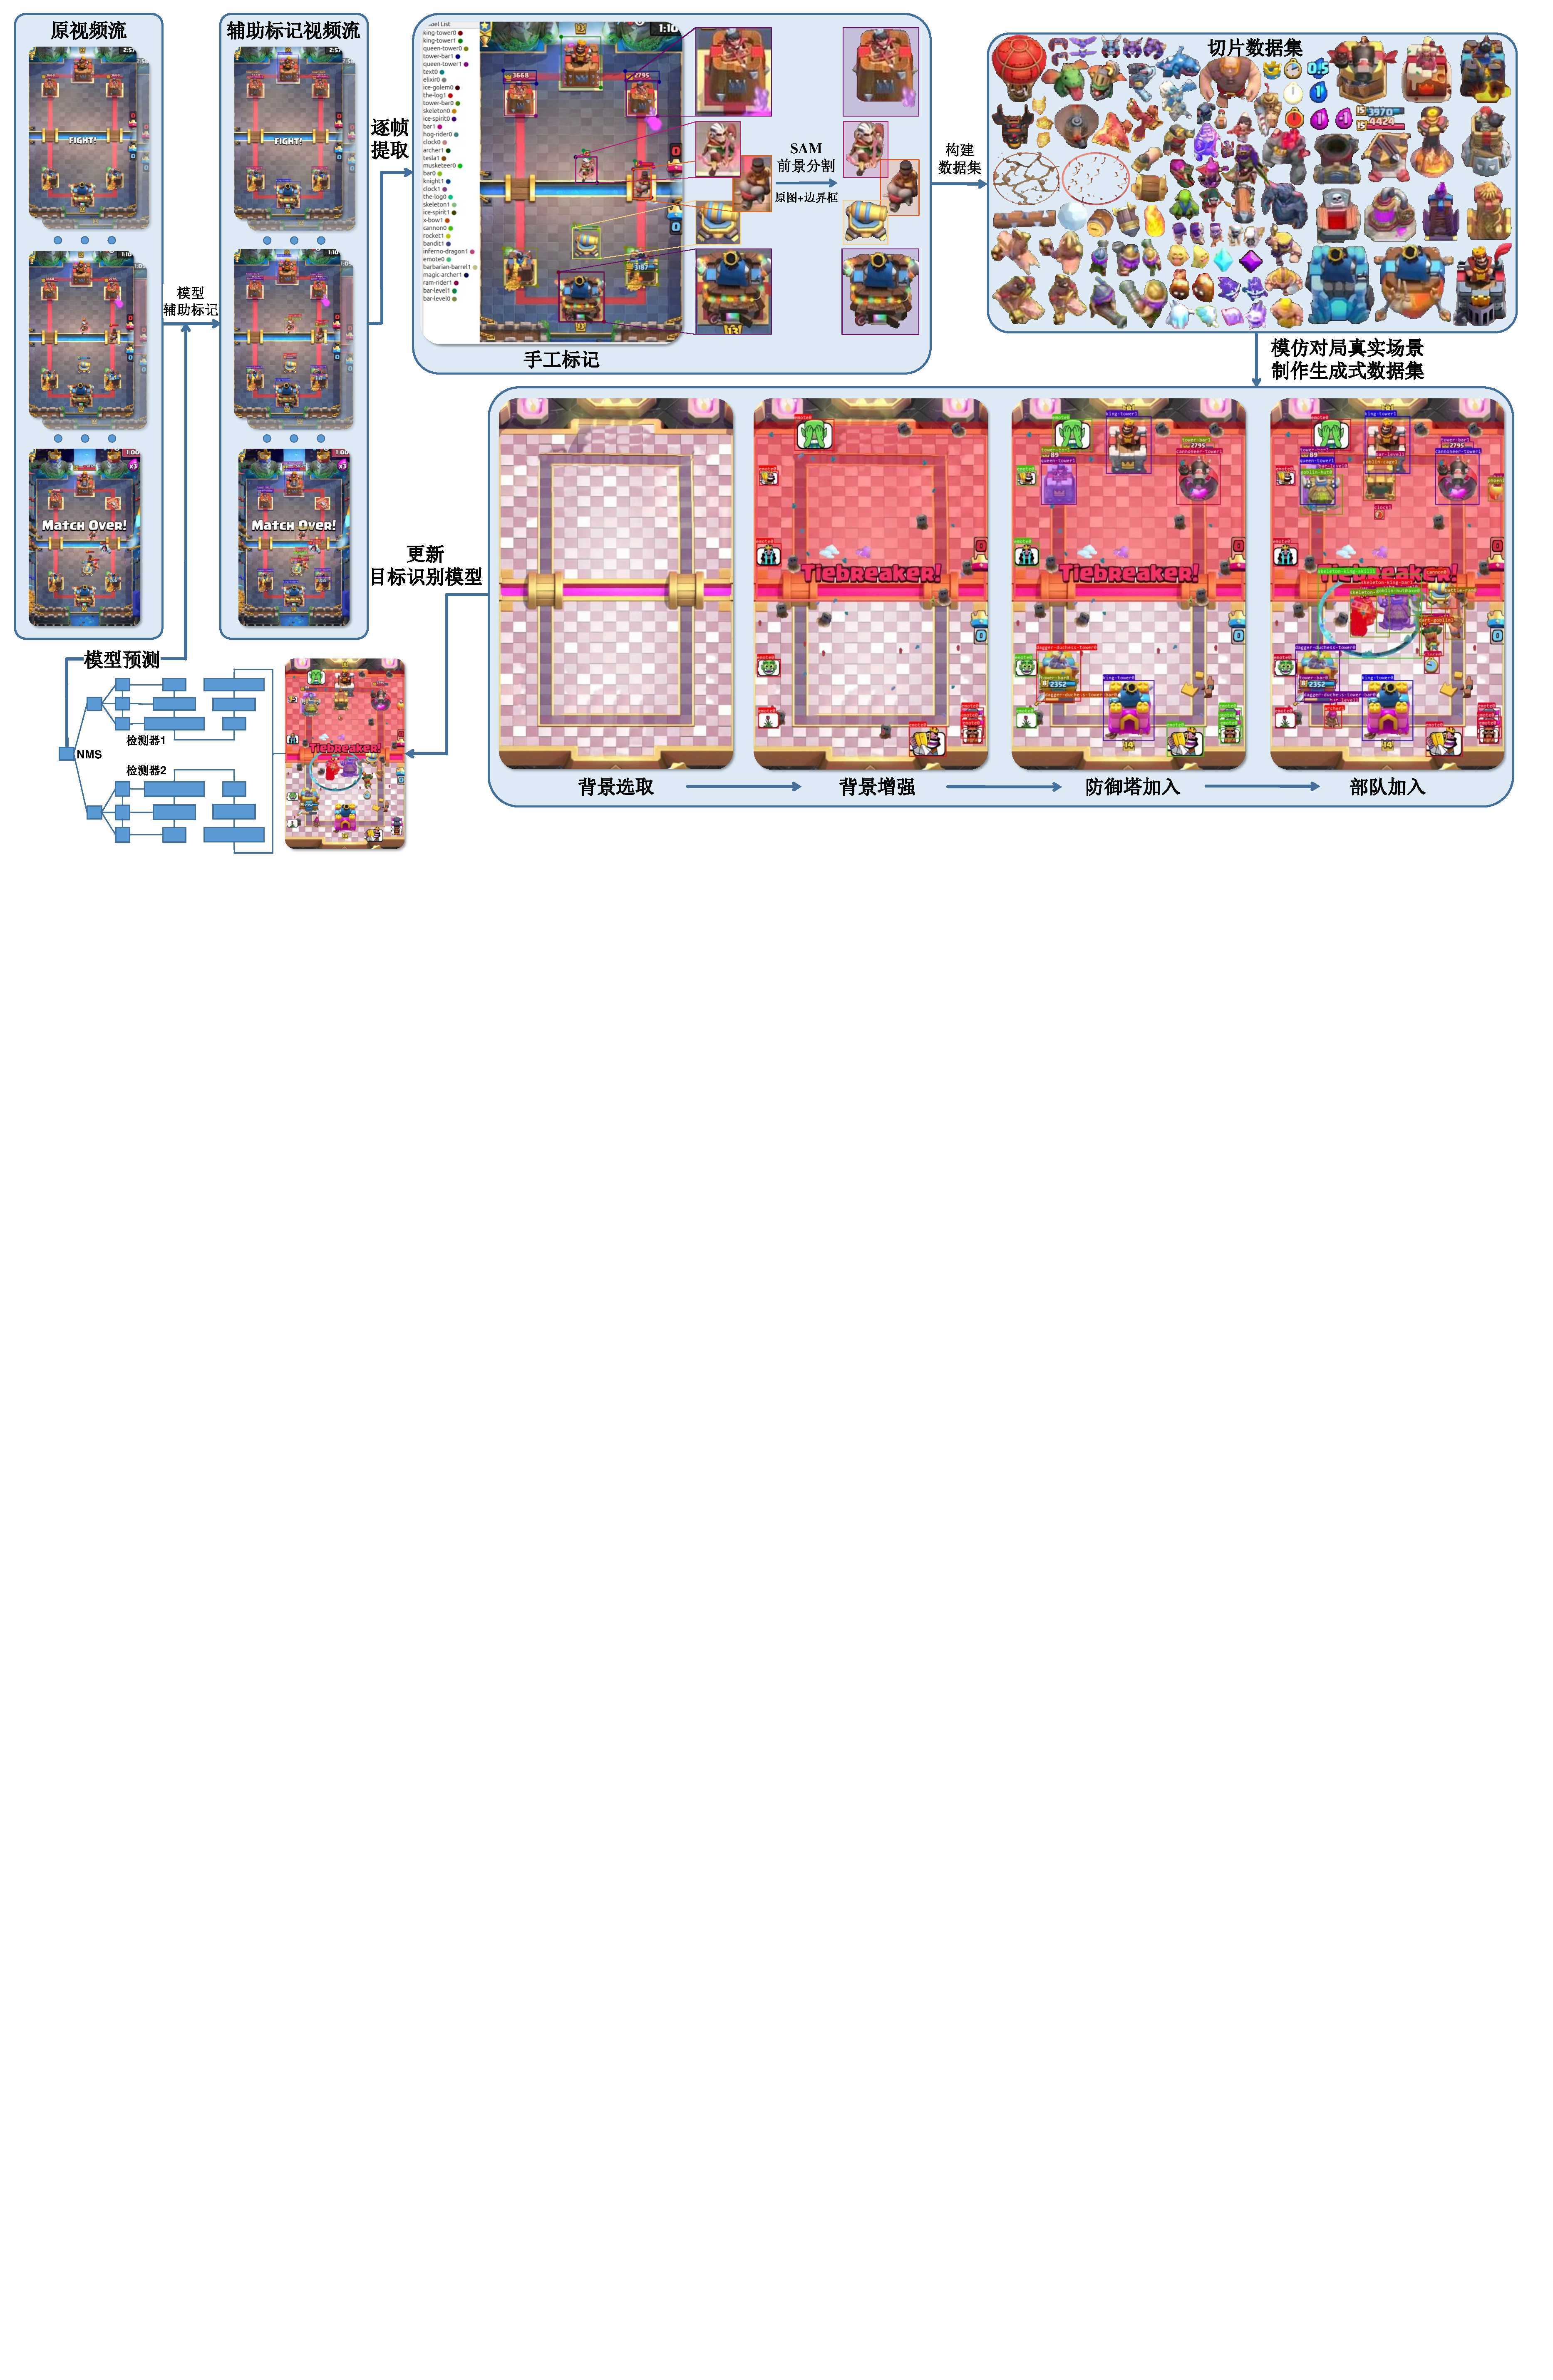
\includegraphics[width=1.0\textwidth]{detection dataset building.pdf}
  \caption{目标识别数据集制作流程:左上部分的“原视频流”为一个回合的视频数据,若存在之前训练的目标识别模型,则
  使用该模型进行对视频流进行辅助标记,获得“辅助标记视频流”再进行手工标记,否则直接对“原视频流”进行手工标记;
  在手工标记中,以0.5秒作为标记间隔,进行人工目标框标记;然后将目标框和原图像同时传入到SAM模型当中获取前景分割,
  将分割后的结果进行人工筛选获得“切片数据集”;基于已完成的切片数据集,利用生成式数据集算法,对目标识别模型进行迭代更新,
  从而用于下一次的辅助标记过程。}
  \label{fig-annotation}
\end{figure}

\BiSection{切片数据集制作流程}{2-1}
切片数据集中制作本毕设使用了一个强大的通用计算机视觉模型:Segment Anything Model (SAM)\upcite{SAM},该模型为Meta AI公司于2023年开源,
该模型可以根据输入的提示信息生成对象的分割掩码,也可对图像中的所有对象生成掩码,
其是在一个包含1100万张图像和11亿各掩码的数据集上进行的训练,能够在很多零样本任务上体现出强大的性能,
SAM模型的核型框架包含如下三个部分:
\begin{enumerate}
  \item 视觉编码器(Vision Encoder):基于ViT的图像特征提取架构,用于捕获图像的上下文信息,将输入图像转化为特征编码。
  \item 提示编码器(Prompt Encoder):用于处理输入中的提示信息,提示信息分为离散(点、框选区域、文本信息)和连续(掩码)两种,
  分别使用位置嵌入(Positional Encoding)和CNN对提示信息进行编码。
  \item 解码器(Decoder):将视觉编码器和提示篇马奇生成的特征进行融合,并输出提示信息所对应的分割掩码。
\end{enumerate}

由于生成式数据集需要获取每一个单位不同角度的切片图像,人工创建分割掩码过于繁琐,但单位的目标框容易标注,
所以考虑使用SAM中框选区域的提示方式生成对象掩码,在图~\ref{fig-annotation}~的中上以及右上部分展示了使用SAM制作切片数据集的过程。

\BiSection{目标识别模型设计}{2-2}
由于需要追求高效的识别速度,所以本文使用了一阶段识别器YOLOv8\upcite{YOLOv8},下面对YOLO系列模型架构进行分析,
并给出本毕设对其进行修改的部分。

\begin{definition}[边界框,Boudning Box]\label{def-iou}
  设正实数$x,y,w,h$,称四元组$B=(x,y,w,h)$为边界框,其中
  $(x,y)$表示当前边界框中心,$(w,h)$表示边界框的宽度和高度。
\end{definition}
\begin{definition}[交并比,Intersection over Union, IOU]
  对于任意两个边界框$B_1,B_2$,分别用$S_1,S_2$表示其所围住的点集,
  则称$B_1,B_2$的交并比为$\text{IOU}_{B_2}^{B_1}:=\frac{S_1\cap S_2}{S_1\cup S_2}$
\end{definition}

设$S,B,C\in\mathbb{Z}^+$分别表示图像网格化大小、每个网格中边界框预测框数目、总分类类别数,通过CNN可以将图像空间进行降维,
从而得到对应的不同网格化大小。例如,在如图~\ref{fig-anchor}~中原图像宽高为$416\times 416$,CNN中每次降采样会将图像的宽高均减小一半,
于是经过步长(Stride)为$s=2^3$的降采样就可以得到左图中$(H/s)\times (W/s) =: S\times S$即$52\times 52$的网格大小,
每个网格中的感受野大小(即步长)即为对应网格中$2^3\times 2^3$个像素,
目标识别模型需要在每个网格处做出$B$个边界框框预测。

图~\ref{fig-anchor}~中,对于每个目标框$B$,其中心点用黄色点标出,假设该中心点位于网格大小为$52\times 52$中的第$(i,j)$网格内,
则在模型预测的输出中,也应该由$(i,j)$网格对应的边界框进行预测。在YOLOv3\upcite{YOLOv3}中,将Fast-RCNN\upcite{FastRCNN}中锚框的概念引入YOLO系列,
对于不同的网格划分,对应分配不同的尺度估计框,称为锚框(Anchor Bounding Box),
这些锚框是基于数据集中的全体锚框做K近邻得到(距离衡量标准为负的相对交并比),可以将数据集中识别框大小的先验信息引入到模型中。
按照网格划分的从大到小,分别分配$B$个从小到大的锚框,
因为更大的网格对应更高的分辨率,其具有更多的细节信息,从而可以识别小目标框,
所以给其分配更小的锚框,反之亦然。

\begin{figure}[htbp]
  \centering
  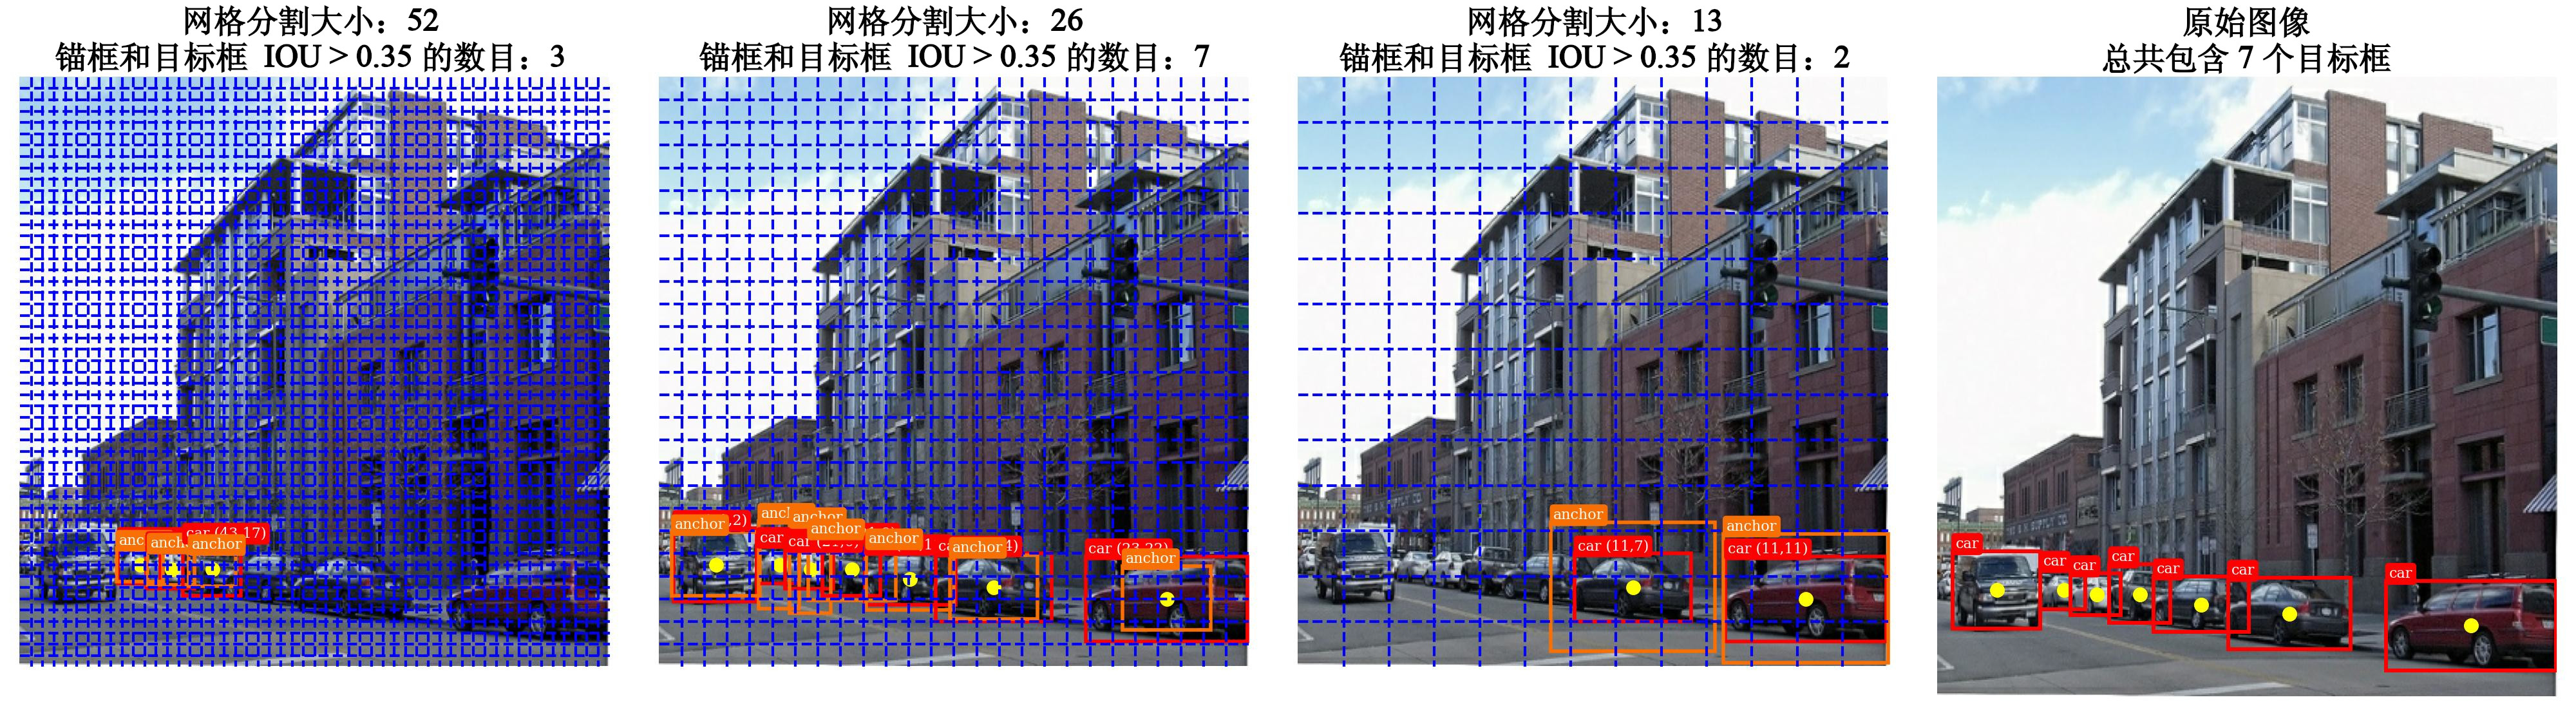
\includegraphics[width=\textwidth]{yolo_anchor_box.jpg}
  \caption{3个不同网格大小下的目标框与锚框,红色为目标框,橙色为基于数据集分配的锚框,
  在3个不同的网格大小下各分配了3种锚框,在图中只显示了相对$\text{IOU}>0.35$的锚框。
  演示的标记图片来自于PASCAL VOC数据集\upcite{PascalVOC}。}
  \label{fig-anchor}
\end{figure}

\begin{definition}[相对预测框]
  假设当前网格步长为$s$,对应的一个锚框为$(A_w,A_h)$,则网格$(i,j)$处的相对预测框定义为六元组$(x,y,w,h,c,\{p_c\}_{c=1}^C, \text{bel})$,其中:
  \begin{itemize}
    \item $(x,y)$表示当前预测框中心点相对于步长$s$的比例,偏移量为$(i\cdot s, j\cdot s)$。
    \item $(w,h)$表示当前预测框的长宽相对于锚框$(A_w,A_h)$的比例。
    \item $c$表示当前预测的置信度,定义为$\text{Pr}(Object)\cdot \text{IOU}_{pred}^{true}$。
    \item $p_c$表示当前预测框预测为类别$c$的概率。
    \item $\text{bel}$表示当前预测框预测从属派别为敌方的概率。
  \end{itemize}
\end{definition}
从上述定义中不难看出,当前网格步长$s$下网格$(i,j)$处的相对预测框所对应的全局边界框为$((j+x)s,(i+y)s, wA_w, hA_h)$。
传统目标识别通常为单类别识别,本毕设任务由于包含单位的从属派别类别,故为多类别识别问题,需要对预测结果以及对应损失函数进行修改。

\begin{definition}[交叉熵损失,Cross-Entropy Loss, CE Loss]\label{def-cross-entropy}
  设模型的输出为$\hat{\bd{z}}\in\mathbb{R}^{N}$,则模型预测分布为(Softmax变换)
  \begin{equation}
    \hat{\bd{y}}_i = \text{softmax}(\bd{z})_i = \frac{\e^{z_i}}{\sum_{j=1}^N\e^{z_j}}
  \end{equation}
  对于$N$维离散目标分布为$\bd{y}\in\mathbb{R}^N$,多元交叉交叉熵损失为
  \begin{equation}\label{eq-ce}
    \mathcal{L}_{CE}(\hat{\bd{y}},\bd{y}) = -\sum_{i=1}^Ny_i\log\hat{y}_{j}
  \end{equation}

  特殊地,当$N=2$时,不妨令目标分布为$\{y, 1-y\}$,则式~\ref{eq-ce}~被称为\textbf{二元交叉熵损失(Binary Cross-Entropy Loss, BCE Loss)}
  \begin{equation}
    \mathcal{L}_{BCE}(\hat{\bd{y}},\bd{y}) = y\cdot \log\hat{\bd{y}}_{1} + (1-y)\cdot \log\hat{\bd{y}}_2
  \end{equation}
\end{definition}
在目标识别任务中目标分布$y$通常为独热分布(Onehot),其中正确预测的概率为$1$,其余类别概率为$0$,
可以表示$\text{onehot}(c) = \{[i=c]\}_{i=1}^C$,$[\text{条件}]$表示当内部条件成立时为$1$,否则为$0$。
然而上述Softmax函数只有当$z_i\gg z_j(i\neq j)$时接近该分布,这会导致模型对其预测过于自行,在目标识别任务中容易出现过拟合现象\upcite{BagFreebiesForObjectDetection}。
\begin{definition}[目标识别损失函数]
设当前网格步长为$s$,输入图像的大小为$W\times H$,每个网格处所需的预测框数目为$B$,\vspace{0.5ex}
第$i$行$j$列网格预测出的第$k$个预测框记为$\left(\widehat{\text{box}}_{ijk},\hat{c}_{ijk}, \hat{p}_{c_{ijk}}, \widehat{\text{bel}}_{ijk}\right)$,
对应的预测框$\left(\text{box}_{ijk}, \text{cls}_{ijk}, \text{bel}_{ijk}\right)$,\vspace{0.5ex}
下面给出该步长下的损失函数
\begin{equation}
\begin{aligned}
\mathcal{L}_{s}(\hat{y}, y) = 
\sum_{i=1}^{H/s}\sum_{j=1}^{W/s}\sum_{k=1}^B&\ \mathbbm{1}^{noobj}_{ijk}\lambda_{noobj}\mathcal{L}_{\text{BCE}}(\hat{c}_{ijk},0)\\
&\ +\mathbbm{1}^{obj}_{ijk}\bigg[\lambda_{\text{box}}\mathcal{L}_{\text{CIOU}}\left(\widehat{\text{box}}_{ijk},\text{box}_{ijk}\right)+
\lambda_{obj}\mathcal{L}_{\text{BCE}}\left(\hat{c}_{ijk},\text{IOU}_{pred}^{true}\right)\\
&\ \qquad\qquad+\lambda_{class}\sum_{c=1}^{C}\mathcal{L}_{\text{BCE}}\bigg(\left\{\hat{p}_{ijk}\right\}_c, \text{onehot}\left(\text{cls}_{ijk}\right)_c\bigg)\\
&\ \qquad\qquad+\lambda_{class}\mathcal{L}_{\text{BCE}}\left(\widehat{\text{bel}}_{ijk}, \text{bel}_{ijk}\right)\bigg]
\end{aligned}
\end{equation}
其中$\mathbbm{1}^{noobj}_{ijk}$当网格$(i,j)$下的第$k$个预测框没有对应的目标框时为$1$,反之为$0$,
相反的$\mathbbm{1}^{obj}_{ijk} = 1-\mathbbm{1}^{noobj}_{ijk}$,
$\mathcal{L}_{\text{CIOU}}$为Complete-IOU损失\upcite{CIOU}是基于IOU损失的一种改进,能够加速边界框回归预测问题中对MSE损失的改进。
\end{definition}

由于本任务的类别数目超过150种,而当前通用目标识别数据集COCO\upcite{COCO}类别为80种,所以本文使用了双模型识别器,如图~\ref{fig-annotation}~中左下角部分,
多个检测器进行组合的模型预测效果见第五章中表~\ref{tabel-yolo}。

\BiSection{生成式目标识别数据集}{2-3}
假设将每个切片作为绘制单位,定义$u = (img,box,level)$,其中$img$为绘制单位的切片图像;
$box=(x,y,w,h,\text{cls},\text{bel})$为绘制单位的边界框参数,$(x,y)$为切片中心点位于图像的二维坐标,
$(w,h)$为切片的宽高大小,cls为当前切片的所属类别,bel为当前切片的所属派别;$level$为当前切片的所属图层等级,
图层等价划分如表~\ref{tab-level}~所示。
\begin{table}[!h]
	\renewcommand{\arraystretch}{1.2}
	\centering\wuhao
	\caption{图层等级与切片类别关系表} \label{tab-level} \vspace{2mm}
	\begin{tabularx}{\textwidth} { 
   >{\centering\arraybackslash}X 
   >{\centering\arraybackslash}X }
	\toprule[1.5pt]
		图层等级 & 切片类别 \\
	\midrule[1pt]
		0 & 地面法术,地面背景部件 \\
		1 & 地面部队,防御塔 \\
		2 & 空中部队,空中法术 \\
		3 & 其余待识别部件,空中背景部件 \\
	\bottomrule[1.5pt]
	\end{tabularx}
\end{table}

绘制单位的插入流程如图~\ref{fig-annotation}~中右下角部分所示,具体细节如下:
\begin{enumerate}
  \item 背景选取:从数据集中随机选取一个去除防御塔、部队及文本信息的空竞技场图片。
  \item 背景增强:加入背景板中的非目标识别部件,用于数据增强,例如:部队阵亡时的圣水,场景中随机出现的蝴蝶、花朵等。
  \item 防御塔加入:在双方的三个防御塔固定点位上随机生成完好或被摧毁的防御塔,并随机选取生成与之相关联的生命值信息。
  \item 部队加入:按照类别出现次数的反比例$\left\{\frac{1}{n_{c_i}-n_{\min}+1}\right\}_{i=1}^{|C|}$\vspace{0.5ex}
  所对应的分布进行类别随机选取,其中$n_{c_i},(c_i\in C)$表示类别$c_i$的切片之前生成的总次数,
  $n_{\min}=\min\{n_{c_i}\}_{i=1}^{|C|}$;在竞技场中按照动态概率分布(具体见附录~\ref{app-dynamic-distrib})随机选择生成点位,
  并随机选取生成与之相关的等级、生命值、圣水、时钟等信息。
\end{enumerate}

\begin{algorithm}[ht]
	\caption{生成算法伪代码\label{alg-generator}}
	\IncMargin{2em}
	\DontPrintSemicolon
	\KwIn{绘制单位序列$U=\{u_i\}$,覆盖率阈值$\alpha$,待识别类别集合$C$}
	\KwOut{image, box}
  $\text{image}\gets$空图像,$\text{box}\gets \{\}$\tcp*{初始化参数}
  $U\gets \{u_i\in U: u_i^{level}>u_j^{level}, \forall i, j \in \{1,\cdots,|U|\} \text{~且~} i < j\}$\;
  \While{True}{
    $\text{mask}\gets$空掩码,$U_{avail}\gets U$\;
    \For{$i=1,2,\cdots,|U|$}{
      \If{$\frac{u^{img}_i\cap~ \text{mask}}{u_i^{img}} > \alpha$}{
        $U_{avail}\gets U_{avail} - R(u_i)$\tcp*{删除与$u_i$相关的单位}
      }
      $\text{mask}\gets \text{mask}\cup u_i^{img}$\;
    }
    \If{$|U_{avail}|=|U|$}{
      break\tcp*{覆盖单位筛选完成}
    }
    $U\gets U_{avail}$
  }
  $U\gets \{u_i\in U: u_i^{level}<u_j^{level}, \forall i, j \in \{1,\cdots,|U|\} \text{~且~} i < j\}$\;
  \For{$i=1,2,\cdots,|U|$}{
    $\text{img}\gets \text{img} \cup u_i^{img}$\tcp*{图像绘制}
    \If{$u_{i}^{\text{cls}}\in C$}{
      $\text{box}\gets \text{box} \cup u_i^{box}$\tcp*{边界框保存}
    }
  }
\end{algorithm}

完成绘制单位加入后,可以按照插入顺序得到待绘制单位序列$U$,但生成的切片可能存在覆盖关系,因此需要引入最大覆盖率阈值$\alpha$,
当被覆盖单位面积超过该单位切片面积的$\alpha$倍时,对被覆盖单位进行去除,对单位完成筛选之后,
再按照图层等级的从高到低进行绘制,并将识别类别$C$中的边界框信息进行记录,用于后续识别模型训练,
具体绘制流程见算法~\ref{alg-generator}。% 通过该生成式算法得到的带标签图像如图~\ref{fig-generation}~所示。
通过调整不同的单位生成数量、切片生成类型,最大覆盖阈值$\alpha$,可以得到如图~\ref{fig-generation}~所示的生成结果
\footnote{生成式代码见附录\ref{app-generator}}。

\begin{figure}[h!]
\centering\vspace{-1.5ex}
\subfigure[单位生成数量20,小型切片类型,$\alpha=0.5$]{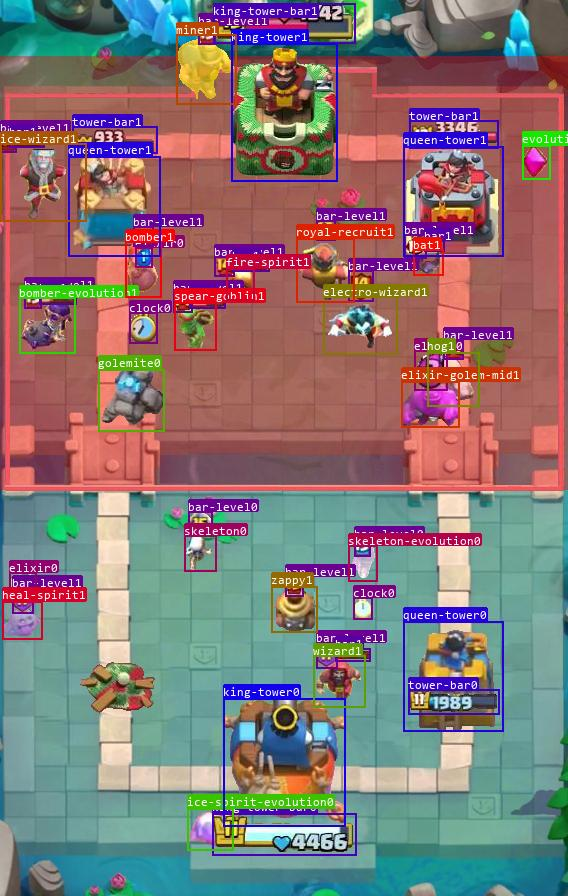
\includegraphics[width=0.32\textwidth]{generation/nu20,small,0.5.jpg}}
\subfigure[单位生成数量20,大型切片类型,$\alpha=0.5$]{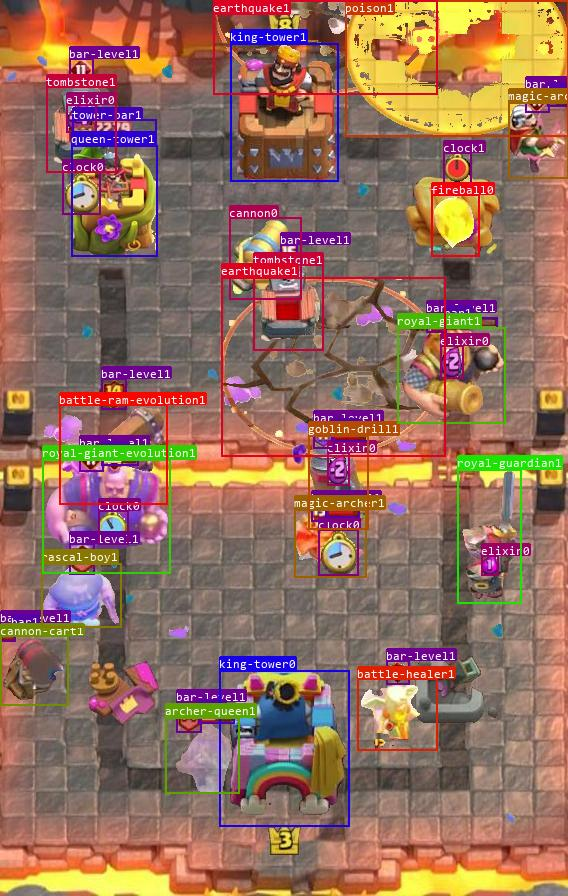
\includegraphics[width=0.32\textwidth]{generation/nu20,big,0.5.jpg}}
\subfigure[单位生成数量20,大型切片类型,$\alpha=0.8$]{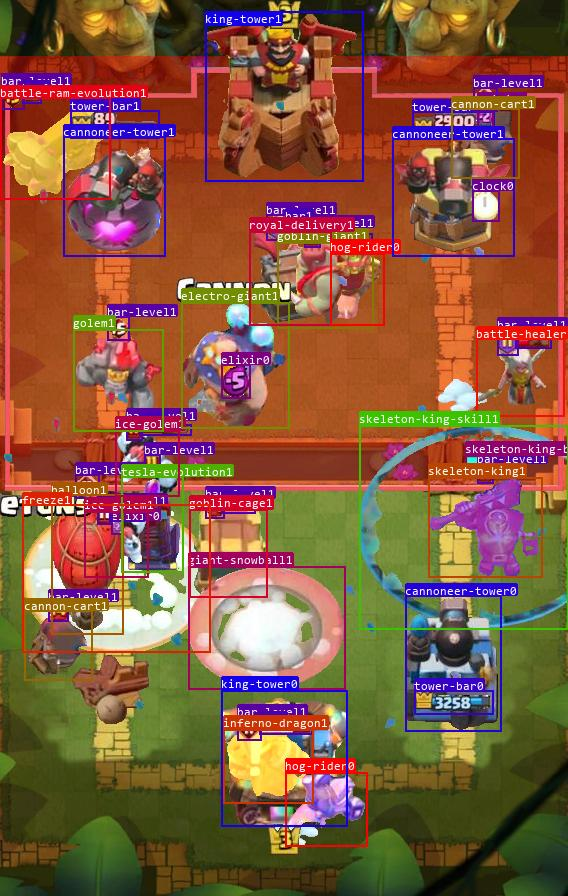
\includegraphics[width=0.32\textwidth]{generation/nu20,big,0.8.jpg}}
\subfigure[单位生成数量40,小型切片类型,$\alpha=0.5$]{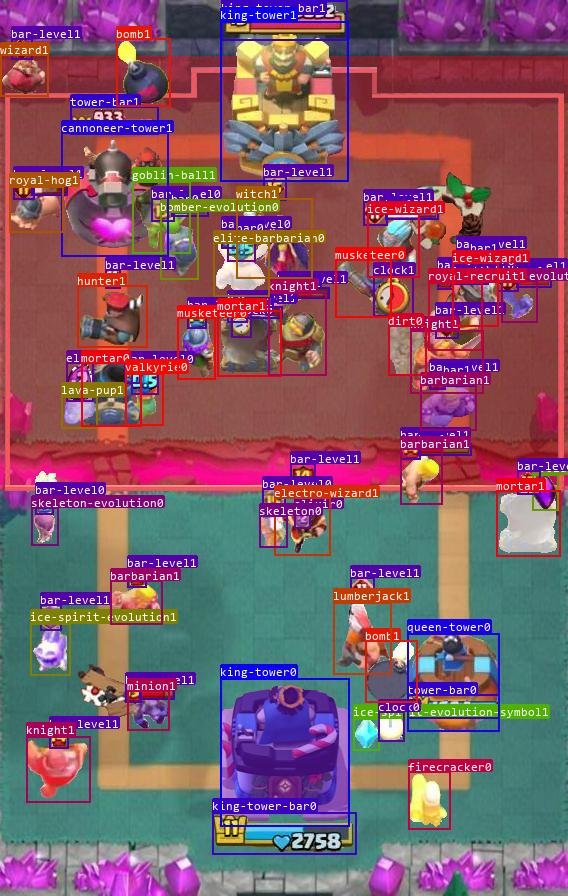
\includegraphics[width=0.32\textwidth]{generation/nu40,small,0.5.jpg}}
\subfigure[单位生成数量40,大型切片类型,$\alpha=0.5$]{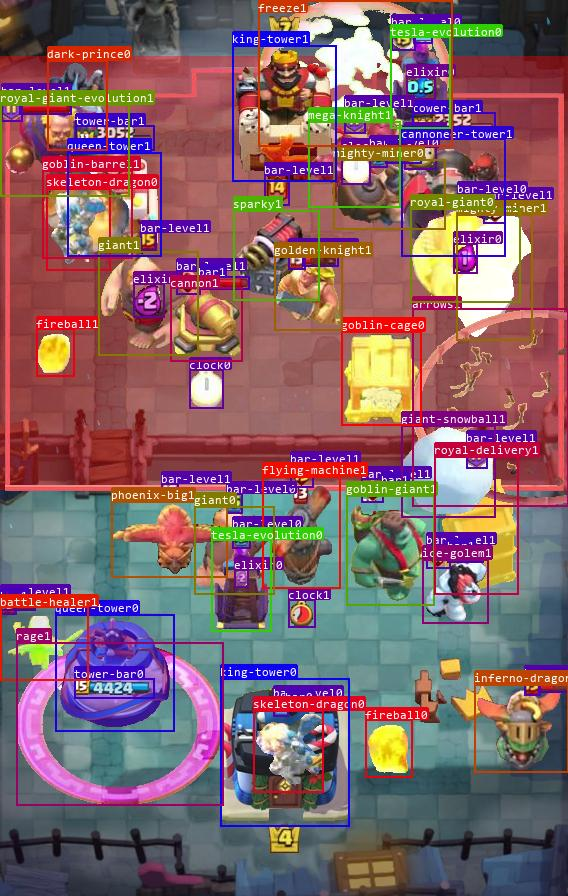
\includegraphics[width=0.32\textwidth]{generation/nu40,big,0.5.jpg}}
\subfigure[单位生成数量40,大型切片类型,$\alpha=0.8$]{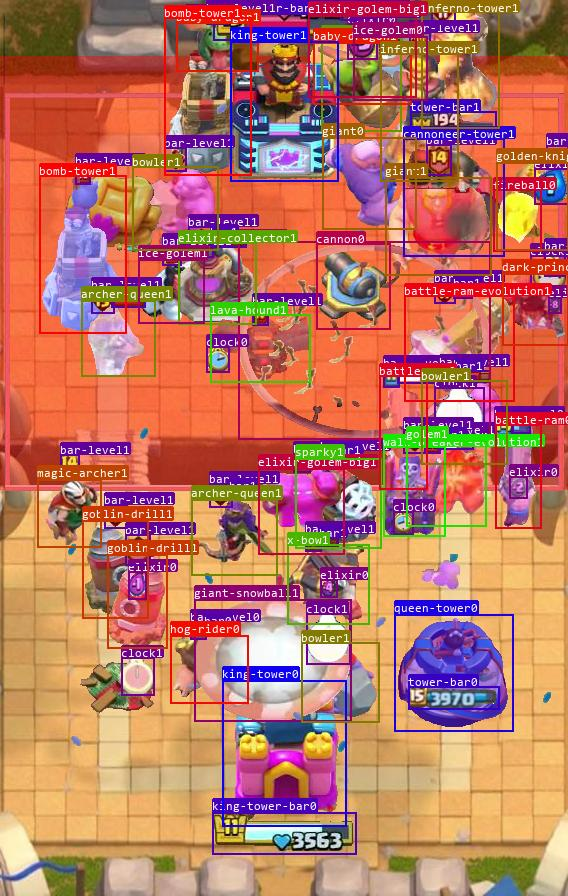
\includegraphics[width=0.32\textwidth]{generation/nu40,big,0.8.jpg}}
\setlength{\abovecaptionskip}{0ex}  % 由于minted会增大图像与标题间距需要进行缩小
\caption{生成式数据集实例}\label{fig-generation}
\end{figure}
  % 正文
% !Mode:: "TeX:UTF-8" 

\BiChapter{图像感知融合与模型决策}{3}\label{chpt-3}
% 本章分别从目标识别、光学字符识别、图像分类三个方面介绍感知提取模型。感知融合结果作为第~\ref{chpt-4}~章决策模型的输入基础,
% 下文分别从状态、动作、奖励特征提取三个方面进行介绍,
% 相关实验结果在~\ref{sec-exp-detect}~中展示。
\BiSection{图像感知模型}{}\label{sec-perceptron}
\BiSubsection{目标识别模型}{}
本文使用YOLO系列模型作为本次目标识别模型,分别尝试了YOLOv5\upcite{YOLOv5}和YOLOv8\upcite{YOLOv8}作为目标识别器,
下面分别对其模型架构改进进行介绍:

YOLOv5主要是对YOLOv4\upcite{YOLOv4}模型进行了少许改进,YOLOv4模型在Backbone部分(初步特征提取)的主要改进
是使用了基于跨阶段部分网络(Cross Stage Partial Networks, CSPNet)\upcite{CSPNet}
结构的DarkNet\upcite{YOLOv3}并在输出特征时使用空间金字塔池化(Spatial Pyramid Pooling,SPP)\upcite{SPP}对特征进行不同尺度上的提取,
在Neck部分(进一步特征提取)中使用了路径聚合网络(Path Aggregation Network, PANet)\upcite{PANet},结合特征金字塔与路径压缩,
缩短了较低层与最顶层特征之间的信息路径,能够有效进行特征融合。

而YOLOv8模型结构上仍然使用CSP和SPP进行特征提取,相对YOLOv5使用了更多的工程优化方法对模型预测速度进行大幅优化,
Head部分(预测框输出)则重新回到YOLOv1\upcite{YOLO}无锚框预测的方法,使预测框不再受到锚框约束。

ByteTrack\upcite{ByteTrack}是一种基于Kalman滤波\upcite{KalmanFilter}的多目标跟踪(Multiple Object Tracking, MOT)算法,
首先需要分别对不同边界框作为跟踪对象,建立独立的线性运动方程,通过Kalman滤波结合之前帧的追踪信息,
以递归的方式给出目标边界框在当前时刻下的位置预测,再通过计算IOU定位当前帧下跟踪对象的位置。
与传统MOT算法不同的是,
ByteTrack尝试利用滤波预测的方法,从更低的置信度对应的边界框中找到可能被忽略的跟踪边界框,
从而恢复可能因遮挡等原因被低估的边界框。

\BiSubsection{光学字符识别模型}{}
PaddleOCR\upcite{PPOCR}是百度公司研发并开源的一个基于PaddlePaddle框架的光学字符识别(Optical Character Recognition, OCR)
系统,PaddleOCR提供了一整套从图像预处理到文字识别的方案,其模型架构主要分为如下两个模块:
\begin{enumerate}
  \item 文本检测模块:使用ResNet\upcite{ResNet}、MobileNet\upcite{MobileNet}等经典的卷积神经网络作为特征提取网络,使用特征金字塔网络(Feature Pyramid Networks,FPN)\upcite{FPN}等方法来融合多尺度特征,
  使用可微分二值化(Differentiable Binarization,DB)\upcite{DB}等方法来预测文本框。
  \item 文本识别模块:使用卷积循环神经网络(Convolutional Recurrent Neural Networks, CRNN)\upcite{CRNN}提取文字区域的特征,
  首先使用卷积网络对图像进行特征提取,再使用Bi-LSTM\upcite{BiLSTM}等序列模型来捕捉字符之间的依赖关系,
  最后使用CTC(Connectionist Temporal Classification)\upcite{CTC}作为文字序列的损失函数。
\end{enumerate}

\BiSubsection{图像分类模型}{}
本毕设的图像分类模型使用ResNet结构,其核心思想是通过引入短连接(Shortcut Connections),
使得网络可以直接学习残差(Residual),从而更容易学习到恒等映射,
缓解深度神经网络中梯度消失的问题。具体来说,ResNet使用残差块(Residual Block)来实现上述操作,
残差块由两部分构成,卷积层:卷积变换$F_W(\cdot)$、批归一化(Batch Normalization, BN)\upcite{BN}以及ReLU激活函数;
残差连接:将输入直接加在卷积层的输出结果上。残差块结构可以表示为
\begin{equation}
  y = \sigma(\text{BN}(F_W(x))) + x,
\end{equation}
其中$x$为输入图像特征,$y$为输出图像特征,$F_W$是以卷积核$W$的卷积变换,BN为批归一化操作,$\sigma(x)=\frac{x+|x|}{2}$为ReLU函数。

\BiSection{图像感知特征提取}{}
在感知特征提取中,本文将同时用到上述三种模型作为一阶段图像特征提取,分别可以得到当前时刻下三个预处理信息:
剩余时间(OCR)、竞技场中的预测框(YOLO)、当前手牌及总圣水(图像分类器)。
下面将介绍特征提取器的设计方法,可以将预处理信息进一步转化为决策模型的输入信息,它们分别为
环境状态信息提取(State)、执行动作信息提取(Action)和环境奖励信息提取(Reward)。
\begin{wrapfigure}[13]{r}{.5\textwidth} % 文字环绕行数为13行, 图片靠右 (l为靠左), 图片占0.5的行宽
  \centering
  \vspace{-1ex}
  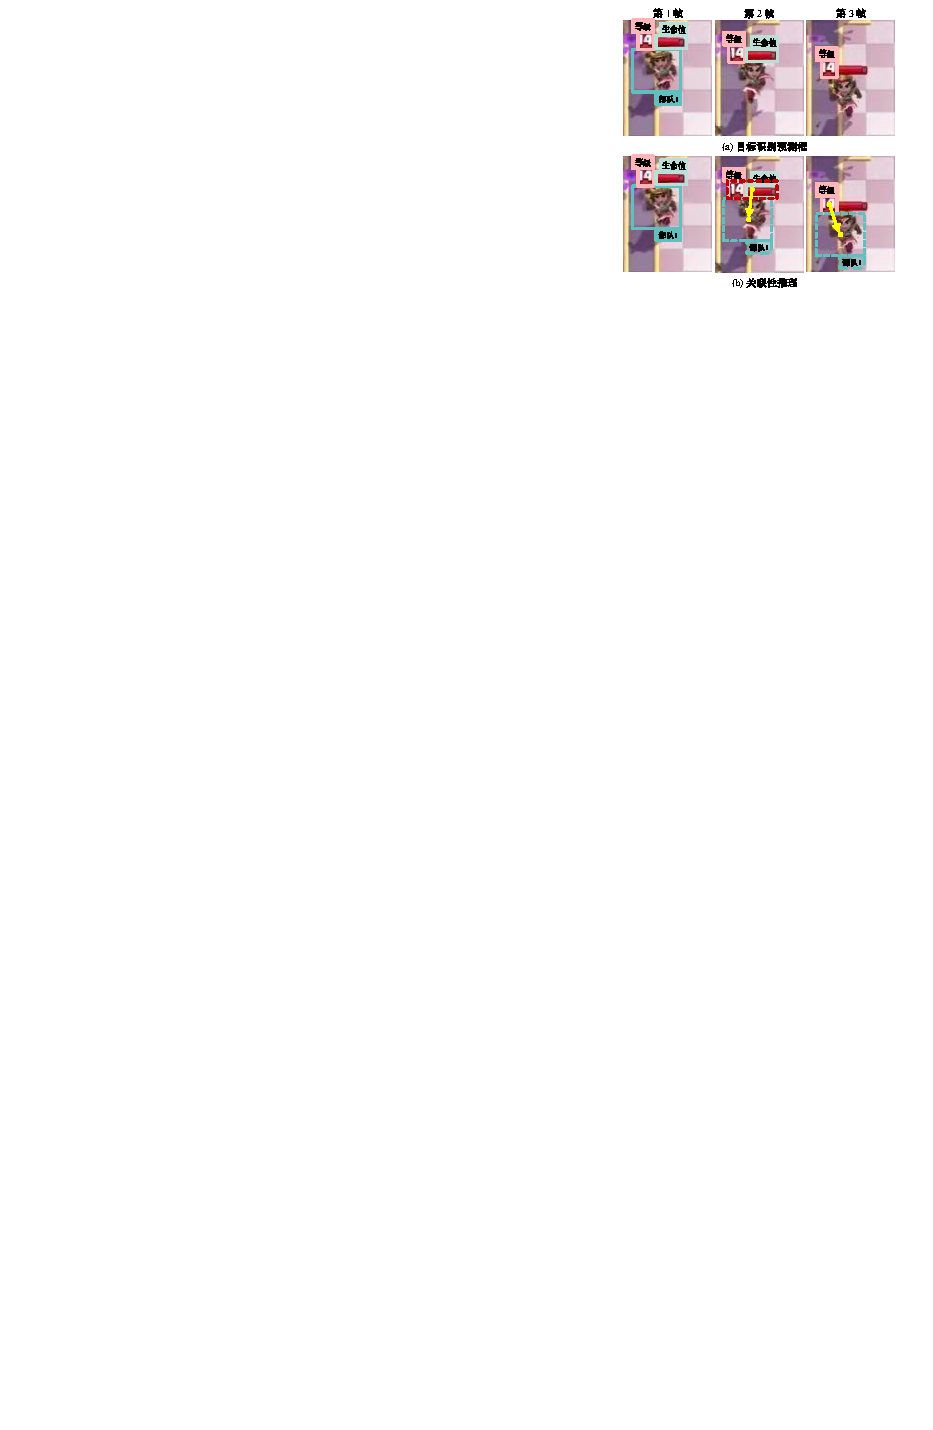
\includegraphics[width=.5\textwidth]{perceptron_improve.pdf}
  \vspace{-1ex}
  \caption{关联性推理}
  \label{fig-state-connect}
\end{wrapfigure}
\vspace{-3ex}
\BiSubsection{状态特征提取}{}
状态特征包括四种信息:
\begin{enumerate}
  \item 经过的总时长:直接通过OCR对图~\ref{fig-introduction}~右上角的阶段剩余时间信息识别后,简单处理即可。
  \item 竞技场中部队信息:每个部队由五个参数构成二维位置坐标、类别、派别、生命值、其余条状信息构成
  $u:=(\boldsymbol{x}, \text{cls}, \text{bel}, \text{bar}_1, \text{bar}_2)$。
  \item 手牌信息:由于手牌可以被拖出但不释放,因此仅识别手牌图像无法确定其真实状态,
  需要通过是否做出动作来判断当前手牌是否被使用,
  故要基于动作特征~\ref{sub-sec-action}~判断当前手牌信息。
\end{enumerate}

\noindent\hspace{1em} 4. 圣水信息:通过OCR对图~\ref{fig-introduction}~下方可用圣水中的数字进行识别。

在竞技场中部队信息特征提取时,本文引入一种基于上下帧关联性推理的方式来解决部队识别错误或漏识别的问题,
在本任务中由于等级和生命值信息容易识别,每个部队都存在一个与之唯一对应的等级和生命值信息,
且部队与等级或生命值信息的相对位置基本不变,所以当部队识别框消失、类别识别错误、派别识别错误时,
利用之前与之关联的等级和生命值信息中进行修正,实现效果如图~\ref{fig-state-connect}~所示。
当模型在第1帧关联了部队1与等级、生命值信息的对应关系,通过目标追踪及上下帧信息记忆,
即使在第2, 3帧未能目标识别模型未能检测到部队1,通过等级或生命值的关联性推理,模型同样可以推理得到当前单位的真实位置。
% \vspace{-3.5ex}
\begin{figure}[htbp]
  \centering\vspace{-1ex}
  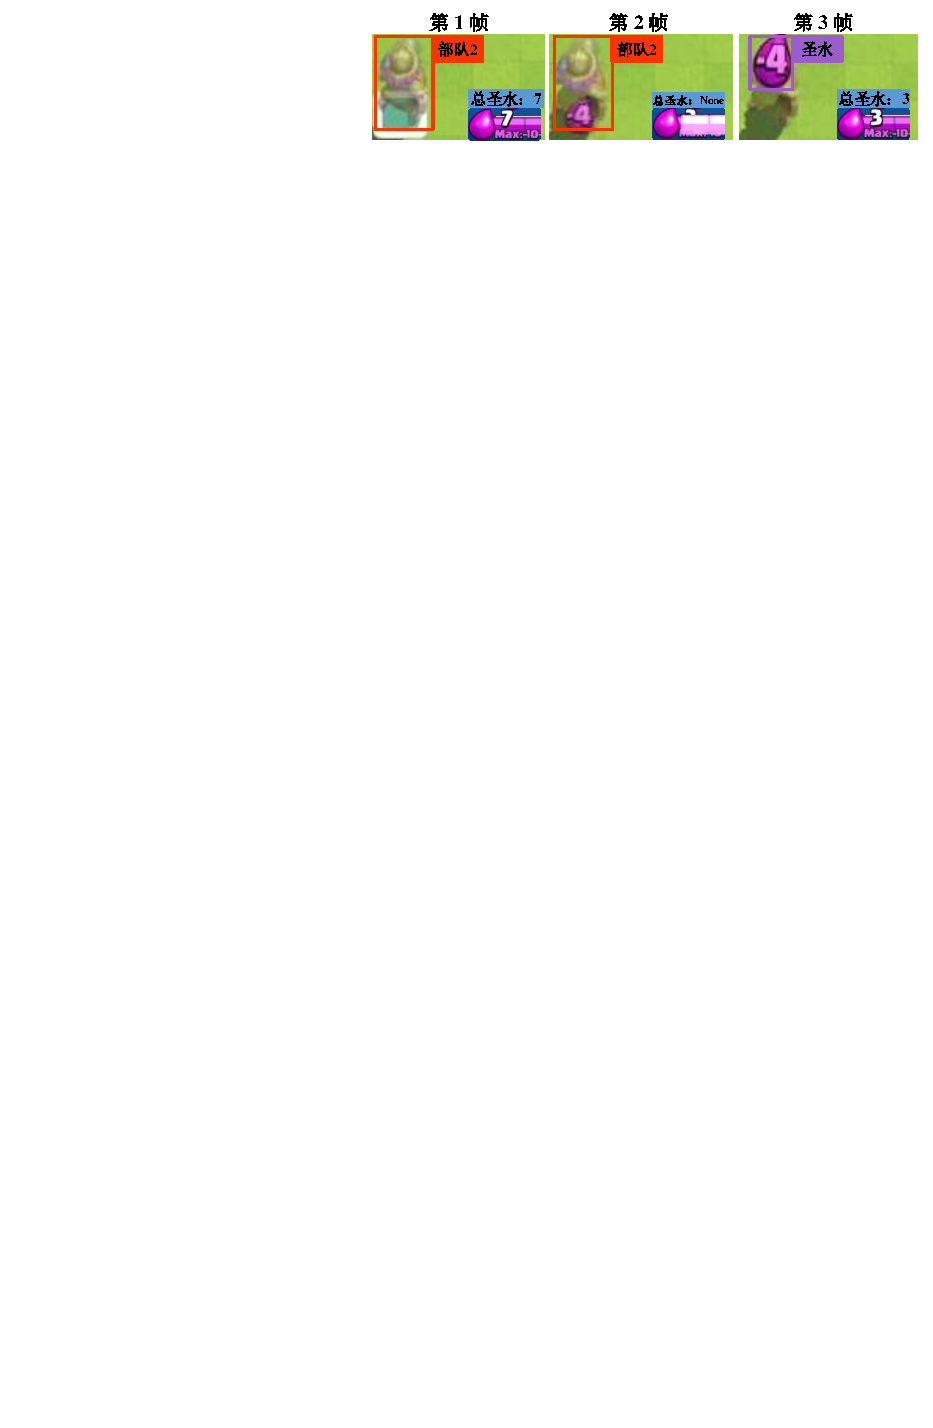
\includegraphics[width=0.8\textwidth]{state_and_action.pdf}
  \vspace{4ex}
  \caption{动作直接导致的错误状态先验信息:第1帧中目标识别错误识别到未部署的部队状态;
  第2帧中OCR识别器在目标识别识别到动作之前,产生了错误的总圣水识别信息,因此需要将动作帧提前到该帧之前;
  第3帧中目标识别成功识别到圣水动画,可以判断玩家在该时刻之前部署了部队。}
  \label{fig-state-action}
\end{figure}
% \begin{wrapfigure}[11]{r}{.6\textwidth} % 文字环绕行数为13行, 图片靠右 (l为靠左), 图片占0.5的行宽
%   \centering
%   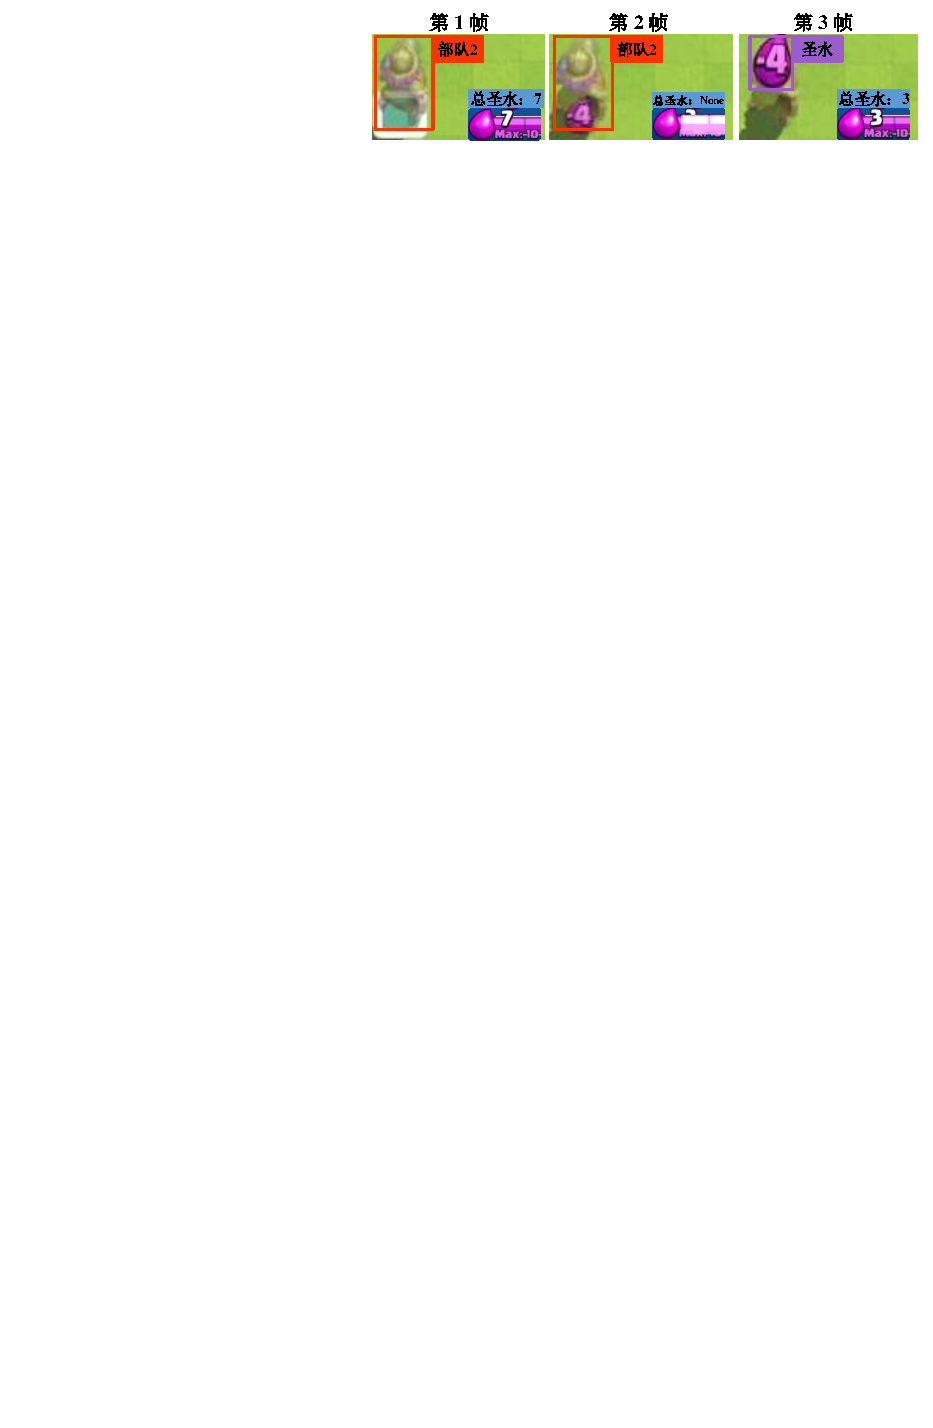
\includegraphics[width=.6\textwidth]{state_and_action.pdf}
%   \caption{动作直接导致的错误状态先验信息:第1帧中目标识别错误识别到未部署的部队状态;
%   第2帧中OCR识别器在目标识别识别到动作之前,产生了错误的总圣水识别信息,因此需要将动作帧提前到该帧之前;
%   第3帧中目标识别成功识别到圣水动画,可以判断玩家在该时刻之前部署了部队。}
%   \label{fig-state-action}
% \end{wrapfigure}

需要注意状态处理的细节问题,在执行动作之前,状态特征中应不包含任何直接与该动作相关的先验信息,
否则模仿学习可以通过该先验信息直接给出动作预测,而真实环境中由于不再出现这类动作的先验信息,
所以导致模型无法做出决策,错误状态信息如图~\ref{fig-state-action}~所示。

假设目标识别每个预测框的识别结果包括七个参数$b:=(x,y,w,h,\text{id},\text{cls},\text{bel})$,
分别为预测框的中心点$(x,y)$,宽高$(w,h)$,目标追踪编号id,预测所属类别cls以及所属派别bel。

\begin{definition}[计数记忆缓存]
  设$I\subset \mathbb{N}$为目标追踪指标集,$S$为可数记忆元素集合,$V\subset \mathbb{R}^+$为可用时间集合,
  定义$M_{T}:I\times S\to\mathbb{Z}^+\times V$为缓存大小为$T$的计数记忆缓存,其满足
  $\forall~ \text{id}\in I, s\in S, (n,t):=M_T(\text{id},s)$,在时间间隔$[t-T,t]\cap V$下追踪指标为id的预测框中,
  存在$n$个预测框包含元素$s$。
\end{definition}

初始化派别记忆缓存$M_{T}^{\text{bel}}$和类别记忆缓存$M_{T}^{\text{cls}}$,其记忆元素集合分别为派别集合$\{0,1\}$
及全体类别集合,假设当前时间为$t$,于是状态特征提取可以分为下述6步\footnote{状态特征提取代码框架见附录~\ref{app-state-feature}~。}:

1. 更新派别记忆缓存:对当前每个预测框$b$,更新$M_{T}^{\text{bel}}(b^{\text{id}}, b^{\text{bel}})$,并对$b^{\text{bel}}$进行修正,
使得$M_T^{\text{bel}}(b^{\text{id}}, b^{\text{bel}})_1 = \max\left\{M_T^{\text{bel}}(b^{\text{id}},x)_1:x\in\{0,1\}\right\}$。

2. 全局文本信息查找:使用OCR对当前竞技场中全部文本信息进行识别,用于解决图~\ref{fig-state-action}~中未放置单位的错误识别问题。

3. 等级、生命值及防御塔信息关联:将等级与部队生命值、防御塔与防御塔生命值进行关联。

4. 部队信息关联:基于贪心的关联策略,从下至上,将部队与在一定范围内最近的等级和生命值进行关联,并基于步骤2结果,去除具有对应文本的部队单位。

5. 缓存清理:将$M_T^{\text{bel}},M_T^{\text{cls}}$中超出时间间隔$[t-T,t]$的信息置零。

6. 更新类别记忆缓存:结合关联性信息,对部队及其关联的等级和生命值信息所对应的$M_T^{\text{cls}}$进行更新,同时对部队类别进行修正,
更新及修正方法与步骤1类似。

\BiSubsection{动作特征提取}{}\label{sub-sec-action}
动作特征包含两种信息:
\begin{itemize}
  \item 当前执行动作的二维坐标$\bd{x}$。
  \item 当前执行动作所用的卡牌编号$\text{card}\in\{1,2,3,4\}$。
\end{itemize}

在进行动作特征提取时,需通过目标识别模型识别到的圣水预测框来判断执行动作的时刻以及坐标位置,
对圣水预测框的目标检测如图~\ref{fig-state-action}~中第3帧所示,但是在第2帧中已经出现了圣水对象,
动作执行本应该发生在第2帧,但是模型无法对其进行识别导致动作判断出现延迟,
所以需通过第2帧中总圣水识别发生突变来进行判断动作的执行,因此需要将第3帧识别到的动作前移至第2帧上。

还需结合当前手牌及圣水上方的文字信息来判断使用的卡牌编号,通过维护一个手牌记忆缓存记录当前可用手牌,
当手牌被玩家或智能体拖出牌库,则将其加入到候选手牌中,每次动作执行的卡牌编号将文本与候选手牌进行比对得到,
当两个文本串的Levenshtein编辑距离\upcite{LevenshteinDistance}不超过2时,则认为两个文本串相同。

初始化圣水记忆缓存$M_{T}^{\text{elixir}}$,其记忆元素集合为可部署单位的二维坐标空间,假设当前时间为$t$,
于是动作特征提取可以分为下述4步\footnote{动作特征提取代码框架见附录~\ref{app-action-feature}~。}:

1. 缓存清理:将$M_{T}^{\text{elixir}}$中超出时间间隔$[t-T,t]$的信息置零。

2. 更新可用手牌及候选手牌:通过手牌分类器的识别结果以及缓存中记录的手牌,可以完成候选手牌、可用手牌的信息更新。

3. 记录总圣水的突变时刻:通过OCR识别当前总圣水以及上一帧总圣水,可用判断当前的总圣水是否发生减少或者无法识别的情况,
当此类情况发生则认为动作执行可能发生在当前帧。

4. 动作查找:通过竞技场中对圣水单位的目标识别,判断动作执行的位置,动作执行的真实时刻为一段时间内最早发生的总圣水突变时刻,
动作卡牌编号需要结合OCR文本识别与候选手牌集合判断,最后再对当前可用手牌进行更新。
\BiSubsection{奖励特征提取}{}
奖励特征仅包含奖励$r\in\mathbb{R}$一种信息,通过OCR识别可以得到敌我防御塔具体生命值,敌我主、副塔如图~\ref{fig-introduction}~中所示,
设$h_{i}^{\text{bel}}, (i\in\{0,1,2\},\text{bel}\in\{0,1\})$为防御塔生命值,
当$i=1,2$时表示左右两个副塔生命值,$i=0$表示主塔生命值,$\text{bel}=0,1$分别表示我方和敌方建筑,
$\Delta h_{i}^{\text{bel}}$表示前一帧与当前帧生命值的差值,$H_{i}^{\text{bel}}$表示对应防御塔的总生命值,分别定义如下四种奖励函数:

1. 防御塔生命值奖励
\begin{equation}
  r_{tower} = \sum_{\text{bel}=0}^1\sum_{i=0}^2(-1)^{\text{bel}+1}\frac{\Delta h_{i}^{\text{bel}}}{H_{i}^{\text{bel}}}
\end{equation}

2. 防御塔摧毁奖励$r_{distory}$:当敌我副塔被摧毁时给予$(-1)^{\text{bel}+1}$奖励,敌我主塔被摧毁时给予前者的$3$倍奖励。

3. 主塔激活奖励$r_{activate}$:当副塔均存活的条件下,主塔第一次失去生命值时,给予$(-1)^{\text{bel}}~0.1$奖励。

4. 圣水溢出惩罚$r_{elixir}$:当总圣水持续保持溢出状态时,每间隔$1$秒产生一次$0.05$的惩罚。

综合上述奖励,得到总奖励\footnote{奖励特征提取代码框架见附录~\ref{app-reward-feature}~。}:
\begin{equation}\label{eq-reward}
  r = r_{tower} + r_{destory} + r_{activate} + r_{elixir}
\end{equation}

需要注意的是,当图像中的数字信息出现噪声干扰或产生错误目标位置识别时,需要终止奖励的错误更新,
例如:部署单位时其他部件对其产生的遮挡(等级、生命值、圣水、时钟、文本)。

\BiSection{决策模型}{}\label{sec-model}
\BiSubsection{离线强化学习}{}\label{sec-offline-rl}
离线强化学习(offline reinforcement learning)是指在没有与环境交互的情况下,
使用预先收集的随机或专家数据来训练强化学习算法,这类算法适用于无法频繁与环境交互或交互代价高昂的场景,
例如自动驾驶、机器人控制等。由于本任务中的非嵌入环境,与环境交互速度效率很低,所以考虑使用离线强化学习作为决策模型。

首先对强化学习中的概念进行介绍,
考虑无限长带折扣Markov决策过程(Markov Decision Process, MDP),定义为$(\mathcal{S},\mathcal{A},p,r,\gamma)$,
其中$\mathcal{S}$为状态空间,$\mathcal{A}$为动作空间,
$p:\mathcal{S}\times \mathcal{A}\times \mathcal{S}\to \mathbb{R}$为状态转移方程,
$r:\mathcal{S}\times\mathcal{A}\to \mathbb{R}$为奖励函数,$\gamma\in(0,1)$为折扣系数。
令$\pi$表示决策函数$\pi: \mathcal{S}\times \mathcal{A}\to [0,1]$,令$R(\pi)$表示其期望所获得的总奖励(回报):
\begin{equation}
  R(\pi) = \mathbb{E}_{S_1,A_1,S_2,A_2\cdots}\left[\sum_{t=0}^{\infty}r(S_t,A_t)\right],\quad
  \text{~其中~}A_t\sim\pi(\cdot|S_t),S_{t+1}\sim p(\cdot|s_t,a_t)
\end{equation}
强化学习的目标通常是找到最优策略$\pi^* := \argmax_{\pi}R(\pi)$,
在线强化学习算法往往通过策略迭代和价值函数估计方法实现策略的更新,
而下文中所使用的离线强化学习算法不再基于值估计方法,而是更加类似于模仿学习的方法。

Decision Transformer(DT)\upcite{DT}是一种将强化学习问题是为序列建模问题的方法,使用了深度学习中的Transformer架构,
对于离线数据集中的一段长度为$T$的交互轨迹(Trajectory)
\begin{equation}
  \rho = (s_1,a_1,r_1,s_2,a_2,r_2,\cdots,s_T,a_T,r_T,s_{T+1}),
\end{equation}
其中$s_{T+1}$为终止状态,则$\rho$可以视为建模为序列
\begin{equation}\label{eq-sequence}
  R_0,s_1,a_1,R_1,s_2,\cdots,a_{T-1},R_{T-1},s_{T},a_{T},
\end{equation}
其中$R_i=\sum_{t=i}^Tr_{t+1}, (i=0,\cdots,T-1)$为目标回报(Return-to-Go)。

DT模型中序列编码模型使用的是GPT模型\upcite{GPT},即仅含有编码器的因果注意力机制。
具体来讲,假设当前处理的序列$X\in\mathbb{R}^{d\times N}$长度为$N$,每个特征编码维度为$d$,
则注意力机制\upcite{attention}包含三个可学习矩阵$W_{Q},W_{K}\in\mathbb{R}^{d_k\times d}, W_{V}\in\mathbb{R}^{d_v\times d}$,
分别对应生成询问键(Query),查询键(Key)和价值键(Value)
\begin{equation}
  \left\{
  \begin{aligned}
  Q=&\ W_{Q}X\\ K=&\ W_{K}X\\ V=&\ W_{V}X
  \end{aligned}
  \right.
\end{equation}
则对于序列中第$i\in\{1,\cdots,N\}$个特征对应的交叉注意力(Cross-Attention)为
\begin{equation}
  \bd{z}^{cross}_i = \sum_{j=1}^N\text{softmax}\left(\left\{\frac{1}{\sqrt{d_k}}\langle \bd{q}_i,\bd{k}_l\rangle\right\}_{l=1}^N\right)_j\cdot \bd{v}_j\iff
  Z^{cross} = \text{softmax}\left(\frac{QK^T}{\sqrt{d_k}}\right)V,
\end{equation}
其中包含系数$1/\sqrt{d_k}$的原因:不妨假设$\bd{q}_{ij}\bd{k}_{lj}\sim \mathcal{N}(0,\sigma^2),~(j\in\{1,\cdots,d_k\})$,
则$\sum_{j=1}^{d_k}\bd{q}_{ij}\bd{k}_{lj}\sim\mathcal{N}(0,d_k\sigma^2)$,由于初始化的神经网络输出可以保证$\sigma\approx 1$,
因此使用系数$1/\sqrt{d_k}$可以保持输出的方差在$1$左右,避免发散。

因果注意力(Causal-Attention)为(每个特征$i$只能看到$j\leqslant i$的特征)
\begin{equation}\label{eq-causal-attn}
\begin{aligned}
  &\ \bd{z}^{causal}_i = \sum_{j=1}^i\text{softmax}\left(\left\{\frac{1}{\sqrt{d_k}}\langle \bd{q}_i,\bd{k}_l\rangle \right\}_{l=1}^N\right)_j\cdot \bd{v}_j\\
  \iff &\ Z^{causal} = \text{softmax}\left(\frac{\left(QK^T\right)\odot M}{\sqrt{d_k}}\right)V,
\end{aligned}
\end{equation}
其中$M$为$N$阶下三角阵,引入因果注意力机制后,每个特征由于无法观察到后续特征,所以可以对相邻的下一个特征进行预测,
从而无需再对编码器和解码器进行区分,降低了代码复杂性。

DT训练方法:首先从离线数据集中随机采样得到一段长度为$N$的轨迹
\begin{equation}
  \tau_{t-N+1:t} =: (R_0,s_1,a_1,R_1,s_2,a_2,\cdots,R_{N-1},s_N,a_N) = \{R_{n-1},s_n,a_n\}_{n=1}^N,
\end{equation}
将每个特征编码到相同维度$\mathbb{R}^d$下,按式~(\ref{eq-sequence})
建模为长度$3N$的序列$\tau\in\mathbb{R}^{3N\times d}$,用GPT模型对序列进行特征编码可以得到和$\tau$维度相同的编码序列$\tau'$,
再取出状态序列所对应的编码结果,通过线性变换映射到动作空间维度,从而得到对相邻动作的预测
\begin{equation}
  (\tau'_2,\tau'_5,\cdots, \tau'_{3N-1})\xrightarrow{\text{~线性变换~}}
  (\hat{a}_1,\hat{a}_2,\cdots,  \hat{a}_{N}).
\end{equation}

对于离散动作空间使用多元交叉熵损失,连续动作空间则使用$\ell^2$范数(Mean Square Error, MSE)作为损失函数。

DT验证方法:需给出模型期望达到的总奖励$\hat{R}_0$,通过自迭代的方式使模型完成动作预测,
具体来说,假设初始状态为$s_1$,则初始轨迹为$\tau_1=(\hat{R}_0,s_1)$,模型对$\tau_1$进行编码,
取出最后一个状态$s_1$所对应的预测动作$\hat{a}_1$与环境交互,
得到新的状态$s_2$和奖励$r_1$,令$\hat{R}_1 = \hat{R}_0 - r_1$,
从而得到新的序列$\tau_2 = (\hat{R}_0,s_1,\hat{a}_1, \hat{R}_1, s_2)$,模型再对$\tau_2$进行编码,
取出$s_2$所对应的预测动作$\hat{a}_2$与环境交互,以此类推,直到环境达到终止状态为止。
这种方式和自然语言模型中文本生成的做法基本一致。

StARformer\upcite{StARformer}是一种基于ViT\upcite{ViT}专门对状态中的图像特征编码进行的改进,
通过将轨迹$\tau$中的$\{(a_{n-1},R_{n-1},s_{n})\}_{n=1}^{3N}$($a_0$使用特征填充补全)
按照空间维度进行展开($s_{n}$使用ViT中图像分块的方法将图像分块序列化),
并压缩到空间特征维度$d'$,进而在空间维度上使用交叉注意力机制进行编码,
得到$\{a'_{n-1},R'_{n-1},s'_{n}\}_{n=1}^{3N}$,
再将第$n$时刻对应的编码$(a'_{n-1},R'_{n-1},s'_{n})$全部展平,
使用线性变换到时间维度$\mathbb{R}^d$中,将其记为$\{l_{n}\}_{n=1}^N$,
则时间维度的序列建模为
\begin{equation}
  \tau:=s_1,l_1,s_2,l_2,\cdots,s_N,l_N
\end{equation}

通过因果注意力机制(相邻的$(s_n,l_n),~n=1,\cdots,N$之间仍然具有注意力机制)可以完成对时序序列信息的编码,
将编码结果记为$\tau'$,
类似DT的预测方法,只考虑所有状态对应的编码结果,
通过线性变换映射到动作空间维度,从而得到相邻动作的预测
\begin{equation}
  (\tau'_1,\tau'_3,\cdots, \tau'_{2N-1})\xrightarrow{\text{~线性变换~}}
  (\hat{a}_1,\hat{a}_2,\cdots, \hat{a}_{N}),
\end{equation}
模型的训练及推理方式与DT完全一致,相比DT模型,StARformer能够有效的提高模型对图像信息的理解能力,
本毕设对上述离线强化学习算法进行了复现\footnote{\url{https://github.com/wty-yy/Decision-Transformer-JAX},
复现内容包括:Decision Transformer(DT),Return-Aligned Decision Transformer(RADT)和StARformer,
在Atari环境中进行了对比试验,并对结果进行可视化。在5个不同Atari环境下的实验表明,StARformer的平均得分超过DT算法的$30\%$。},本文的相关复现实验显示
相比DT更不依赖于初始时目标总奖励$\hat{R}_0$的设定,这说明其更倾向于对专家数据的模仿学习,而非与目标总奖励进行对齐。

\BiSubsection{状态空间与动作空间}{}
模型的状态输入由2部分构成,分别为$S^{img}, \bd{s}^{card}$,其中$S^{img}\in\mathbb{R}^{18\times 32\times 15}$为单位的网格状特征输入,
对于第$i$行$j$列的特征$\bd{z}_{ij}:=(S^{img})_{ij}\in\mathbb{R}^{15}$
表示处于该位置的单位具有如下$4$种特征:$(\bd{z}_{ij})_{1:8}$为类别编码,
$(\bd{z}_{ij})_9$为从属派别编码,$(\bd{z}_{ij})_{10:12}$为生命值图像编码,$(\bd{z}_{ij})_{13:15}$为其余条状图像编码;
$\bd{s}^{card}\in\mathbb{R}^6$表示当前状态下的两个全局特征:$(\bd{s}^{card})_{1:5}$为当前手牌信息,
$(\bd{s}^{card})_6$为当前总圣水量。

模型的动作输入由2个部分构成:$\bd{a}^{pos}, a^{select}$,其中$\bd{a}^{pos}\in\mathbb{R}^2$表示动作执行的部署坐标,
$a^{select}$表示动作执行的手牌编号。

\BiSubsection{预测目标设计与重采样}{}\label{sec-target}
由于本任务中动作执行极为离散,总帧数中仅有$4\%$为执行动作帧,其余帧均不执行动作,
如果直接逐帧预测动作会产生非常严重的长尾问题,导致模型最终基本不执行动作(表~\ref{table-model-eval}~中离散预测的动作数远低于连续动作预测数),
因此需要将预测目标从离散转化为连续,解决方法是引入延迟动作预测:
对于第$i$帧,需找到其后(包含自身)最近的动作帧$j$,令最大间隔帧数阈值为$T_{delay}$,
则每个非动作帧的预测的延迟动作为$a^{delay}_{i} = \min\{j-i, T_{delay}\}$。

对离线数据集进行采样时,为避免长尾问题导致模型偏移,本文还设置了重采样频次,
设数据集总帧数为$N$,动作帧数为$N_{action}$,则动作帧占比为$r_a:=N_{action} / N$,
对于第$i$个动作帧位于数据集中的第$t_i$帧,则$j\in\{t_{i},\cdots,t_{i+1}-1\}$帧作对应的重采样频次为
\begin{equation}\label{eq-resample-freq}
  s_j = \max\left\{\frac{1}{1-r_a}, \frac{1}{r_a(j-t_i+1)}\right\},\quad (t_i\leqslant j\leqslant t_{i+1})
\end{equation}
则训练轨迹中结束帧的采样分布为$\left\{\frac{s_j}{\sum_{j=1}^{N}s_j}\right\}_{j=1}^N$,
图~\ref{fig-resample-and-delay}~中展示了离线数据集一段轨迹所对应的重采样频次与动作预测值。
\begin{figure}[htbp]
  \centering
  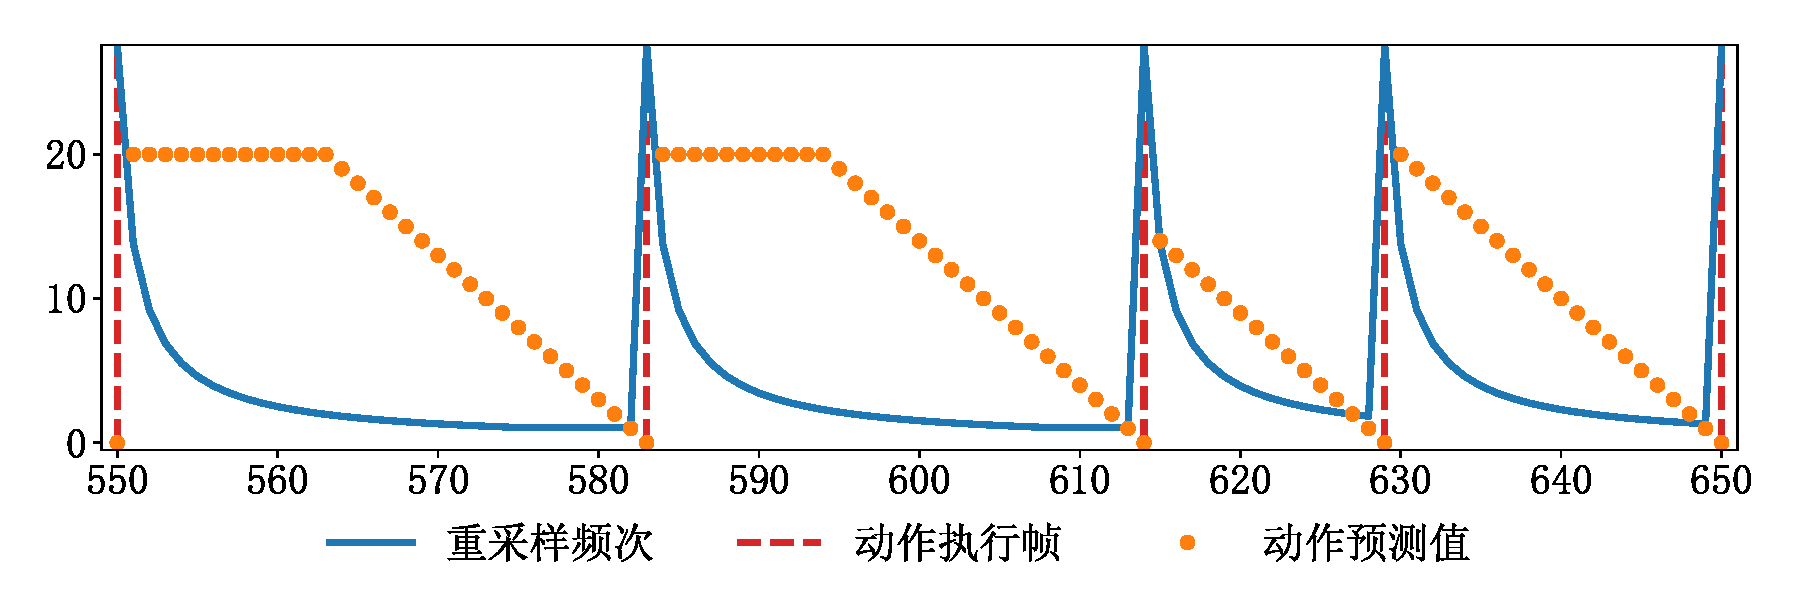
\includegraphics[width=\textwidth]{resample_and_delay.pdf}
  \caption{从离线数据集中截取的一段数据,总共包含5个动作帧,最大间隔帧数阈值$T_{delay} = 20$。}\label{fig-resample-and-delay}
\end{figure}

\BiSubsection{模型架构设计}{}\label{sec-model-struct}
\begin{figure}[htbp]
  \centering\vspace{-2ex}
  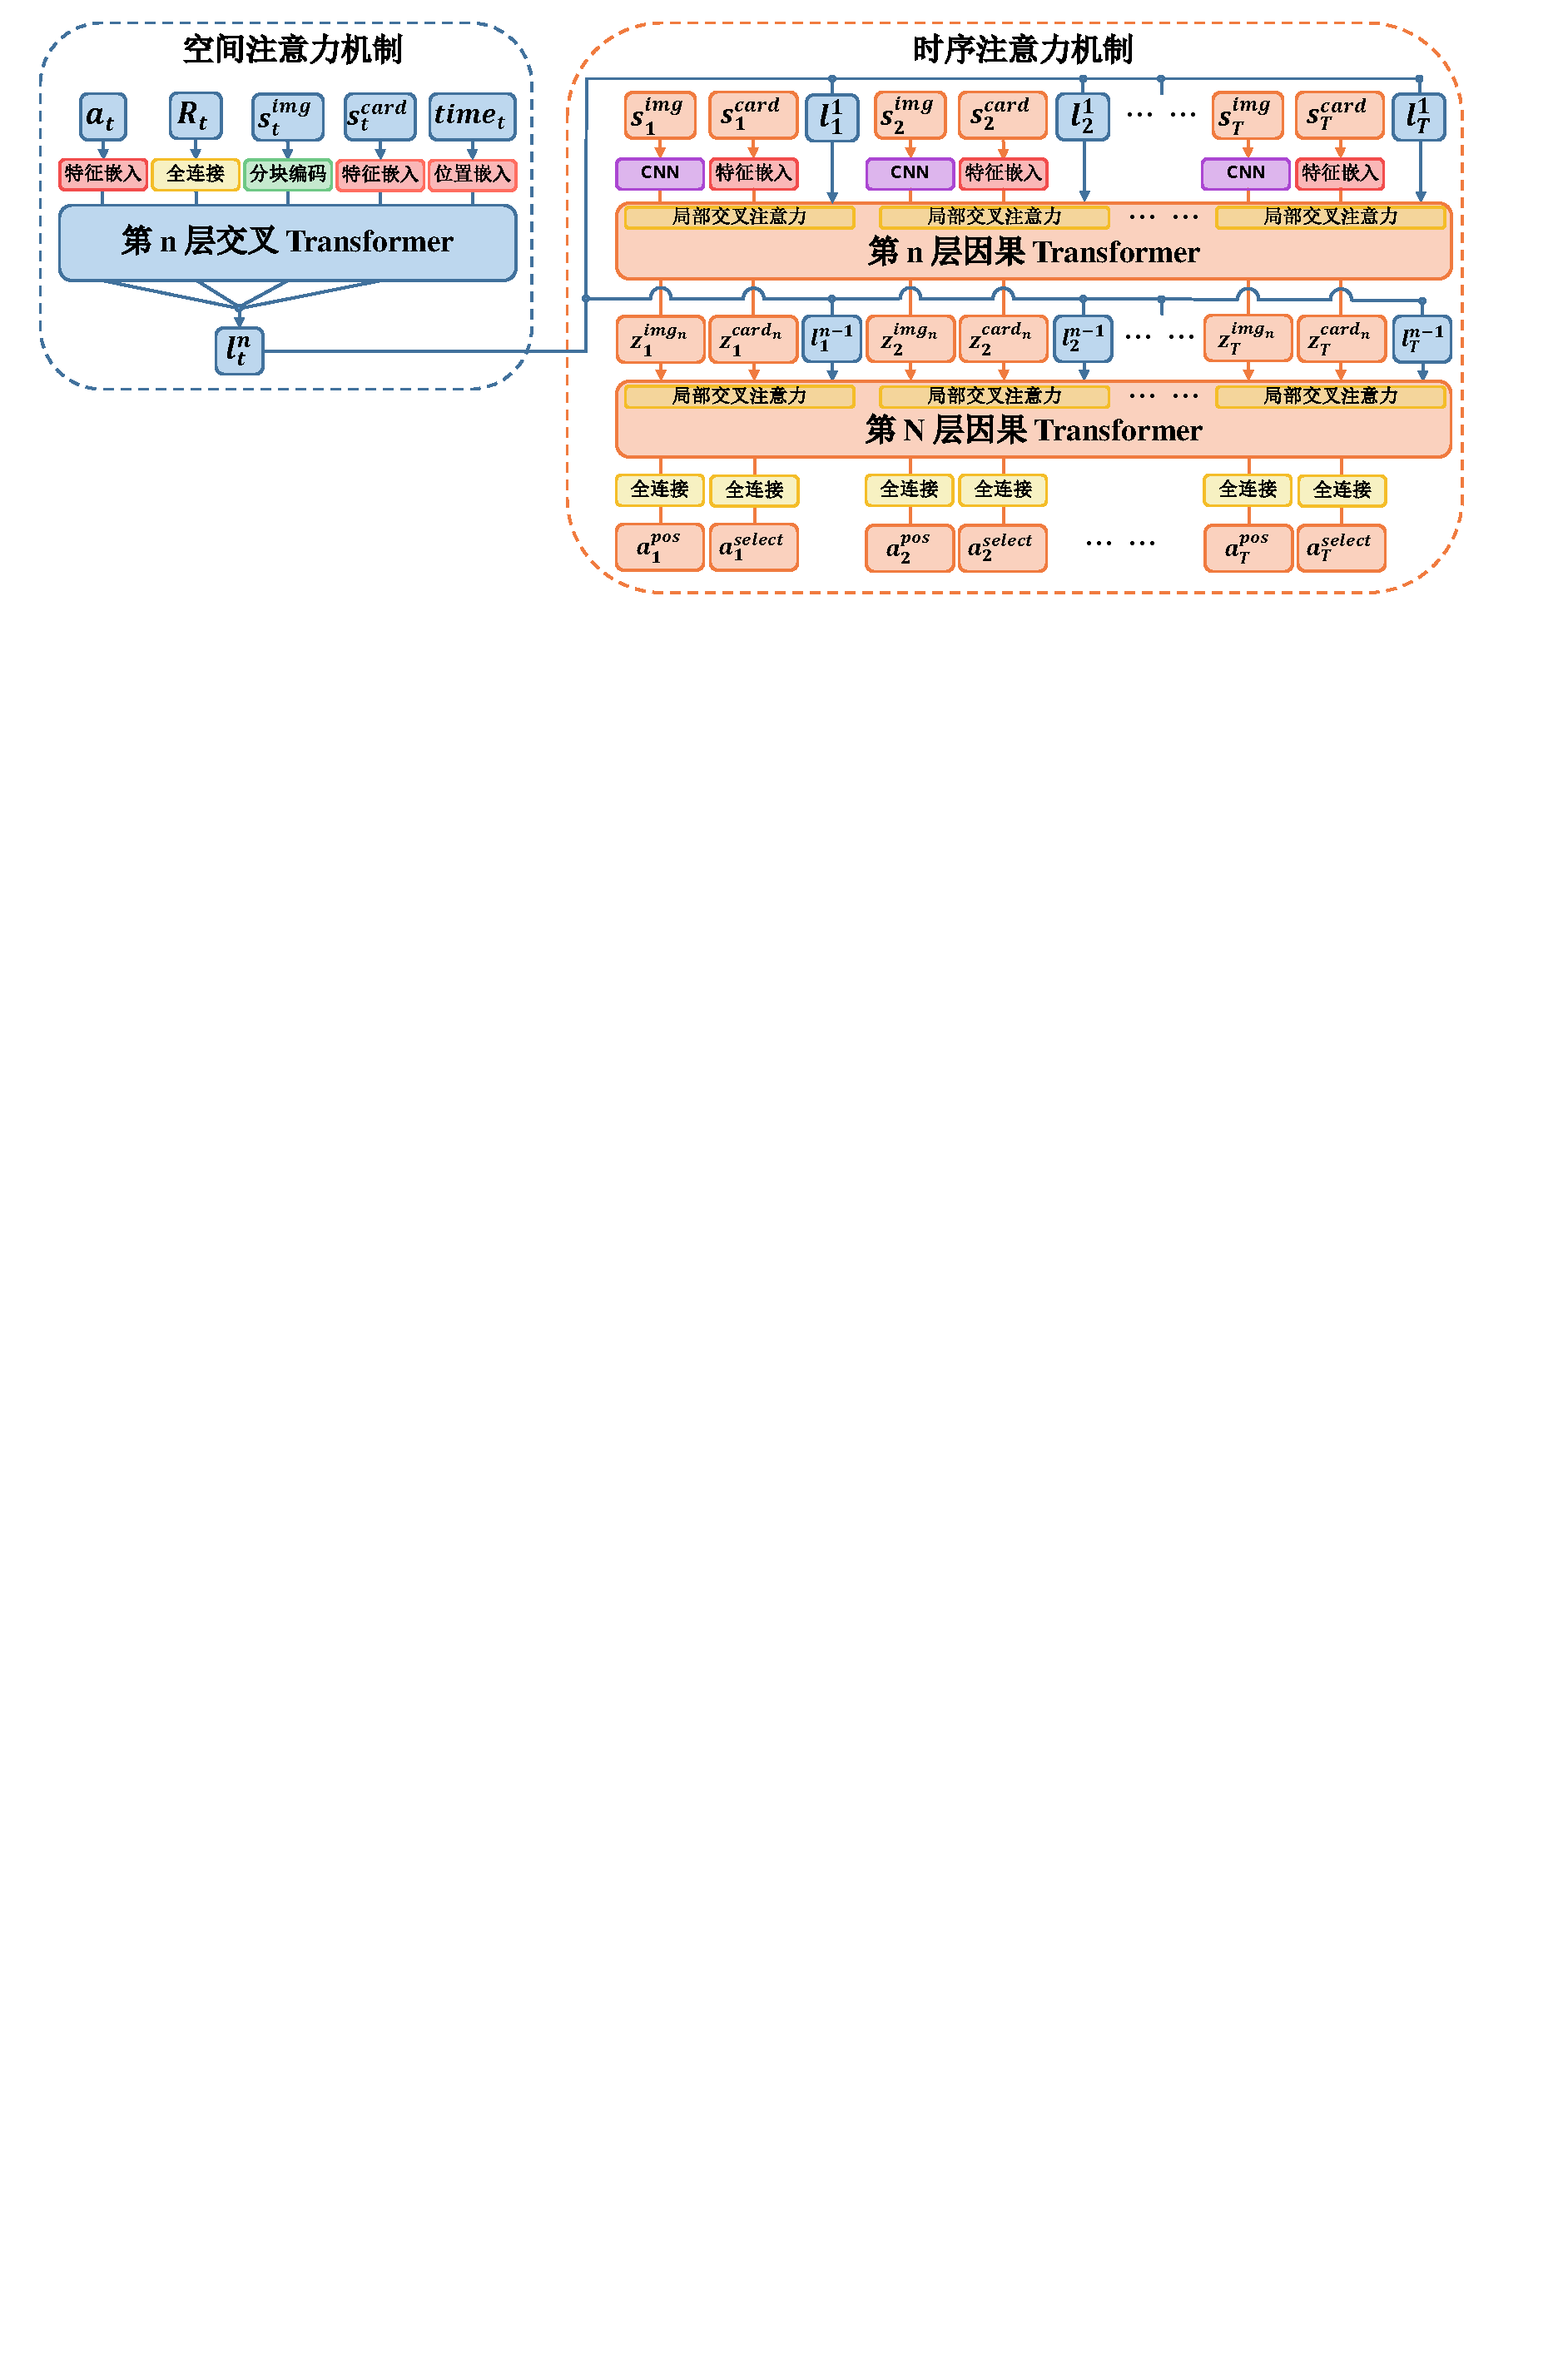
\includegraphics[width=\textwidth]{policy_model.pdf}
  \caption{决策模型架构}
  \label{fig-model}
\end{figure}

本文使用的决策模型架构如图~\ref{fig-model}~所示,基于StARformer的ViT+DT架构,
模型输入为轨迹序列$(a_t, R_t, s_t)_{t=1}^T$,
输出为动作预测序列$(a_t^{pos},a_t^{select})_{t=1}^T$。左侧交叉注意力机制对
局部信息$(a_t,R_t,s_t)$按空间维度进行编码,并使用ViT中分块思路将图像$s_t^{img}$转化为序列;
右侧为因果注意力机制对全局信息$(s^{img}_t,s^{card}_t)$按时序维度进行编码,
并在每层序列输入中引入对应的局部编码信息$l_t^{n}$。

本文总共设计了3种不同的模型架构,分别基于StARformer和DT模型,
假设输入的轨迹长度为$L$,时序注意力机制中的输入序列长度$T$,使用$N$层Transformer堆叠,
则每种模型架构设计细节如下:

StARformer-3L:基于StARformer架构,
本文设计的StARformer-3L决策模型架构如图~\ref{fig-model}~所示,
其中输入序列长度$T=3L$,第$n$层Transformer输出的时序序列记为
$\{z_t^{img_n},z_t^{card_n},l_{t}^{n-1}\}_{t=1}^{L}$(序列长度$3L$)。
右侧时序注意力机制中的因果Transformer,由于需要使同一时刻下的信息可以相互产生注意力关系,
所以需要引入局部交叉注意力,具体实现方法是将式~(\ref{eq-causal-attn})~中的掩码矩阵$M_{3}$,其中$M_{L_0}$定义为
\begin{equation}
  (M_{L_0})_{ij} = \begin{cases}
    1, &\quad i=kL_0-l,j\leqslant kL_0\\
    0, &\quad \text{否则}
  \end{cases},\quad k\in\{1,\cdots,L\}, l\in\{0,\cdots,L_0-1\}
\end{equation}
其本质上是在下三角阵的对角线上顺次放置不交的大小为$L_0\times L_0$的全$1$矩阵。

StARformer-2L:$T=2L$的模型架构与StARformer\upcite{StARformer}论文中架构基本一致,其将图像信息$s_{t}^{img}$与$s_{t}^{card}$编码到同一特征$z_t$中,
得到第$n$层的Transformer输出的时序序列$\{z_t^{n}, l_{t}^{n-1}\}_{t=1}^{L}$(序列长度$2L$),
同理需要使用局部交叉注意力,并将掩码矩阵置为$M_2$,
预测中$a_{t}^{pos}$和$a_{t}^{select}$均使用$z_t$进行解码得到。

DT-4L:基于DT架构,可以看作仅包含图~\ref{fig-model}~中时序注意力部分,
将时序注意力机制中$l_t^{n}$进行替换,得到时序序列为$\{a_{t-1},R_{t-1},s_{t}^{img_n}, s_{t}^{card_n}\}_{t=1}^{L}$(序列长度$4L$),
预测中$a_{t}^{pos}$和$a_{t}^{select}$分别由$s_{t}^{img_n}$和$s_{t}^{card_n}$对应解码得到。

% \BiSection{感知融合小结}{}
% 
% \BiChapter{决策模型}{4}\label{chpt-4}
% 本章首先对离线强化学习中的传统模型进行介绍,再给出本文对模型架构及预测目标的改进内容,
% 相关实验结果在~\ref{sec-decision-model}~中展示。
\BiSection{本章小结}{}
图像感知融合:首先分别对YOLO系列目标识别模型、PaddleOCR光学字符识别模型、ResNet图像分类器进行介绍,将其作为非嵌入图像特征信息的初步提取器,
再通过状态、动作、奖励三种不同感知特征提取器对特征信息进行融合,通过结合上下帧信息及单位的关联信息恢复漏识别目标,
排除对动作决策具有干扰的特征,最后将融合完成的特征作为~\ref{sec-model}~中决策模型的输入信息。

决策模型:先对离线强化学习中的基本定义及DT和StARformer模型进行介绍,详细介绍了训练及推理的实现方法。
由于本任务的离线数据集中存在严重的长尾问题,
本文通过对预测目标的重新设计,并在模型训练中加入重采样策略,从而一定程度上缓解了长尾问题。
最后本文还对StARformer模型架构做出了改进,设计了三种不同的决策模型框架,进行对比实验测试(见表~\ref{table-model-eval})。
从表中可知,预测目标修改提高了$37\%$的模型性能,
将StARformer模型架构从2L修改为3L提高了$24\%$的模型性能。
  % 正文
% % !Mode:: "TeX:UTF-8" 

\BiChapter{决策模型}{4}
\BiSection{离线强化学习}{}\label{sec-offline-rl}
离线强化学习(Offline Reinforcement Learning)是指在没有与环境交互的情况下,
使用预先手机的随机或专家数据来训练强化学习算法,这类算法适用于无法频繁与环境交互或交互代价高昂的场景,
例如自动驾驶、机器人控制等。由于本任务中的非嵌入环境,与环境交互速度效率很低,所以考虑使用离线强化学习作为决策模型。

首先对强化学习中的概念进行介绍,
考虑无限长度的Markov决策过程(MDP),定义为$(\mathcal{S},\mathcal{A},p,r,\rho_0)$,
其中$\mathcal{S}$为状态空间,$\mathcal{A}$为动作空间,
$p:\mathcal{S}\times \mathcal{A}\times \mathcal{S}\to \mathbb{R}$为状态转移方程,
$r:\mathcal{S}\to \mathbb{R}$为奖励函数,$\rho_0:\mathcal{S}\to \mathbb{R}$为初始状态$s_0$对应的分布。

令$\pi$表示决策函数$\pi: \mathcal{S}\times \mathcal{A}\to [0,1]$,令$R(\pi)$表示其期望所获得的总奖励(回报):
\begin{equation}
  R(\pi) = \mathbb{E}_{S_1,A_1,S_2,A_2\cdots}\left[\sum_{t=0}^{\infty}r(S_t)\right],\quad
  \text{~其中~}S_1\sim\rho_0(\cdot),A_t\sim\pi(\cdot|S_t),S_{t+1}\sim p(\cdot|S_t,A_t)
\end{equation}
强化学习的目标通常是找到最优策略$\pi^* := \argmax_{\pi}R(\pi)$,
在线强化学习算法往往通过策略迭代和价值函数估计方法实现策略的更新,
而下文中所使用的离线强化学习算法不再基于值估计方法,而是更加类似于模仿学习的方法。

\BiSubsection{Decision Transformer}{}
Decision Transformer(DT)\upcite{DT}是一种将强化学习问题是为序列建模问题的方法,使用了深度学习中的Transformer架构,
对于离线数据集中的一段长度为$T$的交互轨迹(Trajectory)
\begin{equation}
  \tau = (s_1,a_1,r_1,s_2,a_2,r_2,\cdots,s_T,a_T,r_T,s_{T+1})
\end{equation}
其中$s_{T+1}$为终止状态,则$\rho$可以视为建模为序列
\begin{equation}\label{eq-sequence}
  R_0,s_1,a_1,R_1,s_2,\cdots,a_{T-1},R_{T-1},s_{T},a_{T}
\end{equation}
其中$R_i=\sum_{t=i}^Tr_{t+1}, \quad(i=0,\cdots,T-1)$为目标回报(Return-to-Go)。

DT模型中序列编码模型使用的是GPT模型\upcite{GPT},即仅含有编码器的因果注意力机制。
具体来讲,假设当前处理的序列$X\in\mathbb{R}^{d\times N}$长度为$N$,每个特征编码维度为$d$,
则注意力机制\upcite{attention}包含三个可学习矩阵$Q_{\theta},K_{\theta}\in\mathbb{R}^{d_k\times d}, V_{\theta}\in\mathbb{R}^{d_v\times d}$,
分别对应生成询问键(Query),查询键(Key)和价值键(Value)
\begin{equation}
  Q=Q_{\theta}X,\quad K=K_{\theta}X,\quad V=V_{\theta}X,
\end{equation}
则对于序列中第$i\in\{1,\cdots,N\}$个特征对应的\textbf{交叉注意力(Cross-Attention)}为
\begin{equation}
  \bd{z}^{cross}_i = \sum_{j=1}^N\text{softmax}\left(\left\{\frac{1}{\sqrt{d_k}}\langle \bd{q}_i,\bd{k}_l\rangle\right\}_{l=1}^N\right)_j\cdot \bd{v}_j\iff
  Z^{cross} = \text{softmax}\left(\frac{QK^T}{\sqrt{d_k}}\right)V
\end{equation}
其中包含系数$1/\sqrt{d_k}$的原因:不妨假设$\bd{q}_{ij},\bd{k}_{lj}\sim \mathcal{N}(0,\sigma^2),~(j\in\{1,\cdots,d_k\})$,
则$\sum_{j=1}^{d_k}\bd{q}_{ij}\bd{k}_{lj}\sim\mathcal{N}(0,d_k\sigma^2)$,由于初始化的神经网络输出可以保证$\sigma\approx 1$,
因此使用系数$1/\sqrt{d_k}$可以保持输出的方差在$1$左右,避免发散。

\textbf{因果注意力(Causal-Attention)}为(每个特征$i$只能看到$j\leqslant i$的特征)
\begin{align}
  &\ \bd{z}^{causal}_i = \sum_{j=1}^i\text{softmax}\left(\left\{\frac{1}{\sqrt{d_k}}\langle \bd{q}_i,\bd{k}_l\rangle \right\}_{l=1}^N\right)_j\cdot \bd{v}_j\\
  \iff &\ Z^{causal} = \text{softmax}\left(\frac{\left(QK^T\right)\odot M}{\sqrt{d_k}}\right)V,\quad
  \text{~其中~}M\text{~为~}N\text{~阶下三角阵~}\label{eq-causal-attn}
\end{align}
引入因果注意力机制后,每个特征由于无法观察到后续特征,所以可以对相邻的下一个特征进行预测,
从而无需再对编码器和解码器进行区分,降低了代码复杂性。

DT训练方法:首先从离线数据集中随机采样得到一段长度为$N$的轨迹
\begin{equation}
  \tau_{t-N+1:t} =: (s_1,a_1,r_1,s_2,a_2,r_2,\cdots,s_N,a_N,r_N) = \{(s_n,a_n,R_n)\}_{n=1}^N
\end{equation}

再每个特征编码到相同维度$\mathbb{R}^d$下,按式~\ref{eq-sequence}
建模为长度$3N$的序列$\tau\in\mathbb{R}^{3N\times d}$,用GPT模型对序列进行特征编码可以得到和$\tau$维度相同的编码序列$\tau'$,
再取出状态序列所对应的编码结果,通过线性变换映射到动作空间维度,从而得到对相邻动作的预测
\begin{equation}
  \tau'_2,\tau'_5,\cdots, \tau'_{3k-1},\cdots,\tau'_{3N-1}\xrightarrow{\text{~线性变换~}}
  \hat{a}_1,\hat{a}_2,\cdots, \hat{a}_{k},\cdots, \hat{a}_{N}
\end{equation}

对于离散动作空间使用定义~\ref{def-cross-entropy}~中的多元交叉熵损失,
连续动作空间则使用$\ell^2$范数(Mean Square Error, MSE)作为损失函数。

DT验证方法:需给出模型期望达到的总奖励$\hat{R}_0$,通过自迭代的方式时模型完成动作预测,
具体来说,假设初始状态为$s_1$,则初始轨迹为$\tau_1=(\hat{R}_0,s_1)$,模型对$\tau_1$进行编码,
取出最后一个状态$s_1$所对应的预测动作$\hat{a}_1$与环境交互,
得到新的状态$s_2$和奖励$r_1$,令$\hat{R}_1 = \hat{R}_0 - r_1$,
从而得到新的序列$\tau_2 = (\hat{R}_0,s_1,\hat{a}_1, \hat{R}_1, s_2)$,模型再对$\tau_2$进行编码,
取出$s_2$所对应的预测动作$\hat{a}_2$与环境交互,以此类推,直到环境达到终止状态为止。
这种方式和自然语言模型中文本生成的做法基本一致。

\BiSubsection{StARformer}{}\label{sec-starformer}
StARformer\upcite{StARformer}是一种基于ViT\upcite{ViT}专门对状态中的图像特征编码进行的改进,
通过将轨迹$\tau$中的$\{(a_{n-1},r_{n-1},s_{n})\}_{n=1}^{3N}$($a_0$使用特征填充补全)
按照空间维度进行展开($s_{n}$使用图像分块的方法将图像分块序列化),
并压缩到空间特征维度$d'$,进而在\textbf{空间维度}上使用交叉注意力机制进行编码,
得到$\{(a'_{n-1},r'_{n-1},s'_{n})\}_{n=1}^{3N}$,
再将第$n$时刻对应的编码$(a'_{n-1},r'_{n-1},s'_{n})$全部展平,
使用线性变换到时间维度$\mathbb{R}^d$中,将其记为$\{l_{n}\}_{n=1}^N$,
则\textbf{时间维度}的序列建模为
\begin{equation}
  \tau:=s_1,l_1,s_2,l_2,\cdots,s_N,l_N
\end{equation}

通过因果注意力机制(相邻的$(s_n,l_n),~n=1,\cdots,N$之间仍然具有注意力机制)可以完成对时序序列信息的编码,
将编码结果记为$\tau'$,
类似DT的预测方法,只考虑所有状态对应的编码结果,
通过线性变换映射到动作空间维度,从而得到相邻动作的预测
\begin{equation}
  \tau'_1,\tau'_3,\cdots, \tau'_{2k-1},\cdots,\tau'_{2N-1}\xrightarrow{\text{~线性变换~}}
  \hat{a}_1,\hat{a}_2,\cdots, \hat{a}_{k},\cdots, \hat{a}_{N}
\end{equation}
模型的训练及推理方式与DT完全一致,相比DT模型,StARformer能够有效的提高模型对图像信息的理解能力,
本毕设对上述离线强化学习算法进行了复现\footnote{\url{https://github.com/wty-yy/Decision-Transformer-JAX},
复现内容包括:Decision Transformer(DT),Return-Aligned Decision Transformer(RADT)和StARformer,
在Atari环境中进行了对比试验,并对结果进行可视化。},本文的相关复现实验显示
相比DT更不依赖于初始时目标总奖励$\hat{R}_0$的设定,这说明其更倾向于对专家数据的模仿学习,而非与目标总奖励进行对齐,
在5个不同Atari环境下的实验表明,StARformer的平均得分超过DT算法的$30\%$。

\BiSection{决策模型设计}{}\label{sec-model}
\BiSubsection{状态空间与动作空间}{}
模型的状态输入由2部分构成,分别为$S^{img}, \bd{s}^{card}$,其中$S^{img}\in\mathbb{R}^{18\times 32\times 15}$为单位的网格状特征输入,
对于第$i$行$j$列的特征$\bd{z}_{ij}:=(S^{img})_{ij}\in\mathbb{R}^{15}$
表示处于该位置的单位具有如下$4$种特征:$(\bd{z}_{ij})_{1:8}$为类别编码,
$(\bd{z}_{ij})_9$为从属派别编码,$(\bd{z}_{ij})_{10:12}$为生命值图像编码,$(\bd{z}_{ij})_{13:15}$为其余条状图像编码;
$\bd{s}^{card}\in\mathbb{R}^6$表示当前状态下的两个全局特征:$(\bd{s}^{card})_{1:5}$为当前手牌信息,
$(\bd{s}^{card})_6$为当前总圣水量。

模型的动作输入由2个部分构成:$\bd{a}^{pos}, a^{select}$,其中$\bd{a}^{pos}\in\mathbb{R}^2$表示动作执行的部署坐标,
$a^{select}$表示动作执行的手牌编号。

\BiSubsection{预测目标设计与重采样}{}\label{sec-target}
由于本任务中动作执行极为离散,总帧数中仅有$4\%$为执行动作帧,其余帧均不执行动作,
如果直接逐帧预测动作会产生非常严重的长尾问题,导致模型最终基本不执行动作(表~\ref{table-model-eval}~中离散预测的动作数远低于连续动作预测数),
因此需要将预测目标从离散转化为连续,解决方法是引入延迟动作预测:
对于第$i$帧,需找到其后(包含自身)最近的动作帧$j$,令最大间隔帧数阈值为$T_{delay}$
则每个非动作帧的预测的延迟动作为$a^{delay}_{i} = \min\{j-i, T_{delay}\}$。

对离线数据集进行采样时,为避免长尾问题导致模型偏移,本文还设置了重采样频次,
设数据集总帧数为$N$,动作帧数为$N_{action}$,则动作帧占比为$r_a:=N_{action} / N$,
对于第$i$个动作帧位于数据集中的第$t_i$帧,则$j\in\{t_{i},\cdots,t_{i+1}-1\}$帧作对应的重采样频次为
\begin{equation}\label{eq-resample-freq}
  s_j = \max\left\{\frac{1}{1-r_a}, \frac{1}{r_a(j-t_i+1)}\right\},\quad (t_i\leqslant j\leqslant t_{i+1})
\end{equation}
则训练轨迹中结束帧的采样分布为$\left\{\frac{s_j}{\sum_{j=1}^{N}s_j}\right\}_{j=1}^N$,
图~\ref{fig-resample-and-delay}~中展示了离线数据集一段轨迹所对应的重采样频次与动作预测值。
\begin{figure}[htbp]
  \centering
  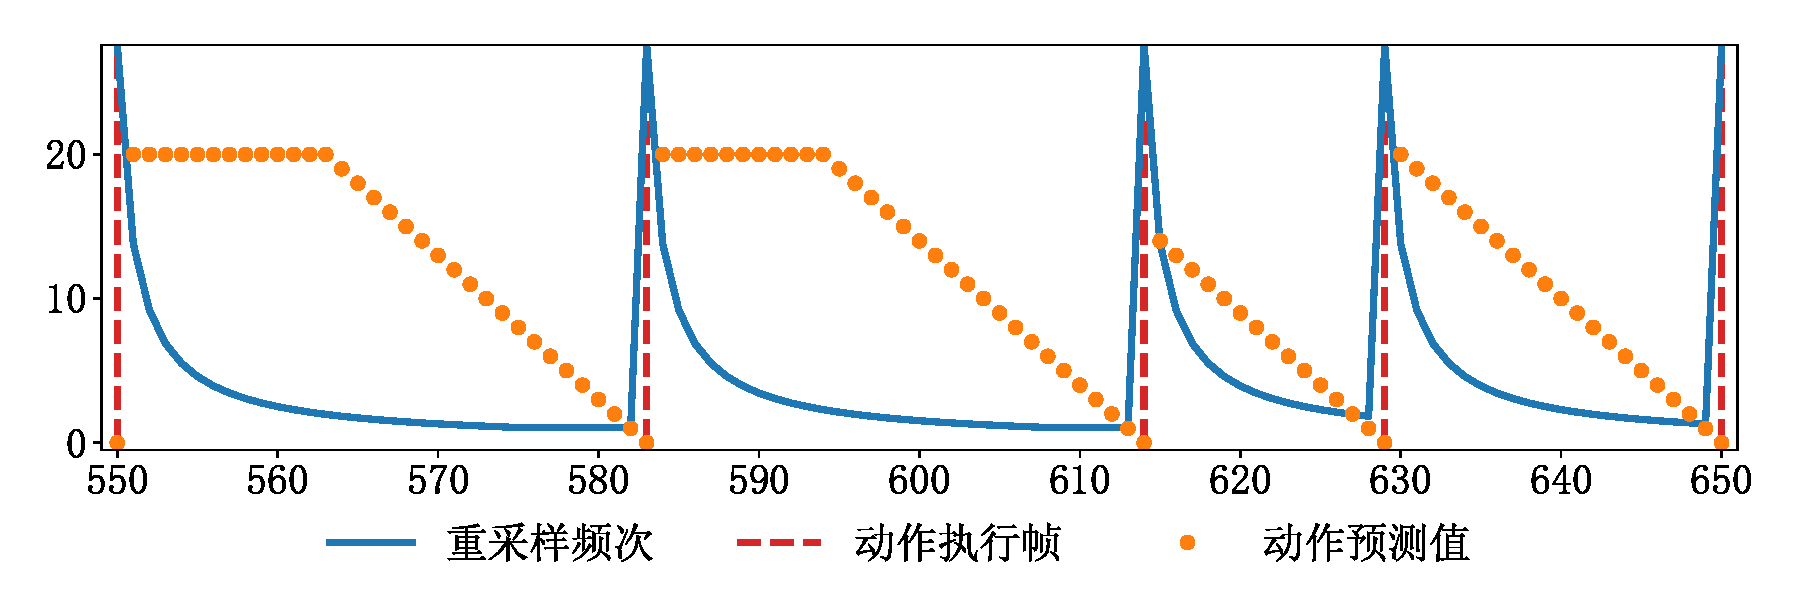
\includegraphics[width=\textwidth]{resample_and_delay.pdf}
  \caption{从离线数据集中截取的一段数据,总共包含5个动作帧,最大间隔帧数阈值$T_{delay} = 20$,}\label{fig-resample-and-delay}
\end{figure}

\BiSubsection{模型架构设计}{}\label{sec-model-struct}
本文设计了3种不同的模型架构,分别基于StARformer和DT模型,
假设输入的轨迹长度为$L$,时序注意力机制中的输入序列长度$T$,使用$N$层Transformer堆叠,
则每种模型架构设计细节如下:

StARformer-3L:基于StARformer架构,
本文设计的StARformer-3L决策模型架构如图~\ref{fig-model}~所示,
其中输入序列长度$T=3L$,第$n$层Transformer输出的时序序列记为
$\{z_t^{img_n},z_t^{card_n},l_{t}^{n-1}\}_{t=1}^{L}$(序列长度$3L$)。
右侧时序注意力机制中的因果Transformer,由于需要使同一时刻下的信息可以相互产生注意力关系,
所以需要引入局部交叉注意力,具体实现方法是将式~\ref{eq-causal-attn}~中的掩码矩阵$M_{3}$,其中$M_{L_0}$定义为
\begin{equation}
  (M_{L_0})_{ij} = \begin{cases}
    1, &\quad i=kL_0-l,j\leqslant kL_0\\
    0, &\quad \text{否则}
  \end{cases},\quad \big(k\in\{1,\cdots,L\}, l\in\{0,\cdots,L_0-1\}\big)
\end{equation}
其本质上是在下三角阵的对角线上顺次放置不交的大小为$L_0\times L_0$的全$1$矩阵。

StARformer-2L:$T=2L$的模型架构与StARformer\upcite{StARformer}论文中架构基本一致,其将图像信息$s_{t}^{img}$与$s_{t}^{card}$编码到同一特征$z_t$中,
得到第$n$层的Transformer输出的时序序列$\{z_t^{n}, l_{t}^{n-1}\}_{t=1}^{L}$(序列长度$2L$),
同理需要使用局部交叉注意力,并将掩码矩阵置为$M_2$,
预测中$a_{t}^{pos}$和$a_{t}^{select}$均使用$z_t$进行解码得到。

DT-4L:基于DT架构,可以看作仅包含图~\ref{fig-model}~中时序注意力部分,
将时序注意力机制中$l_t^{n}$进行替换,得到时序序列为$\{a_{t-1},R_{t-1},s_{t}^{img_n}, s_{t}^{card_n}\}_{t=1}^{L}$(序列长度$4L$),
预测中$a_{t}^{pos}$和$a_{t}^{select}$分别由$s_{t}^{img_n}$和$s_{t}^{card_n}$对应解码得到。

上述各种模型及不同预测目标的验证比对结果请见表~\ref{table-model-eval}~。

\begin{figure}[htbp]
  \centering
  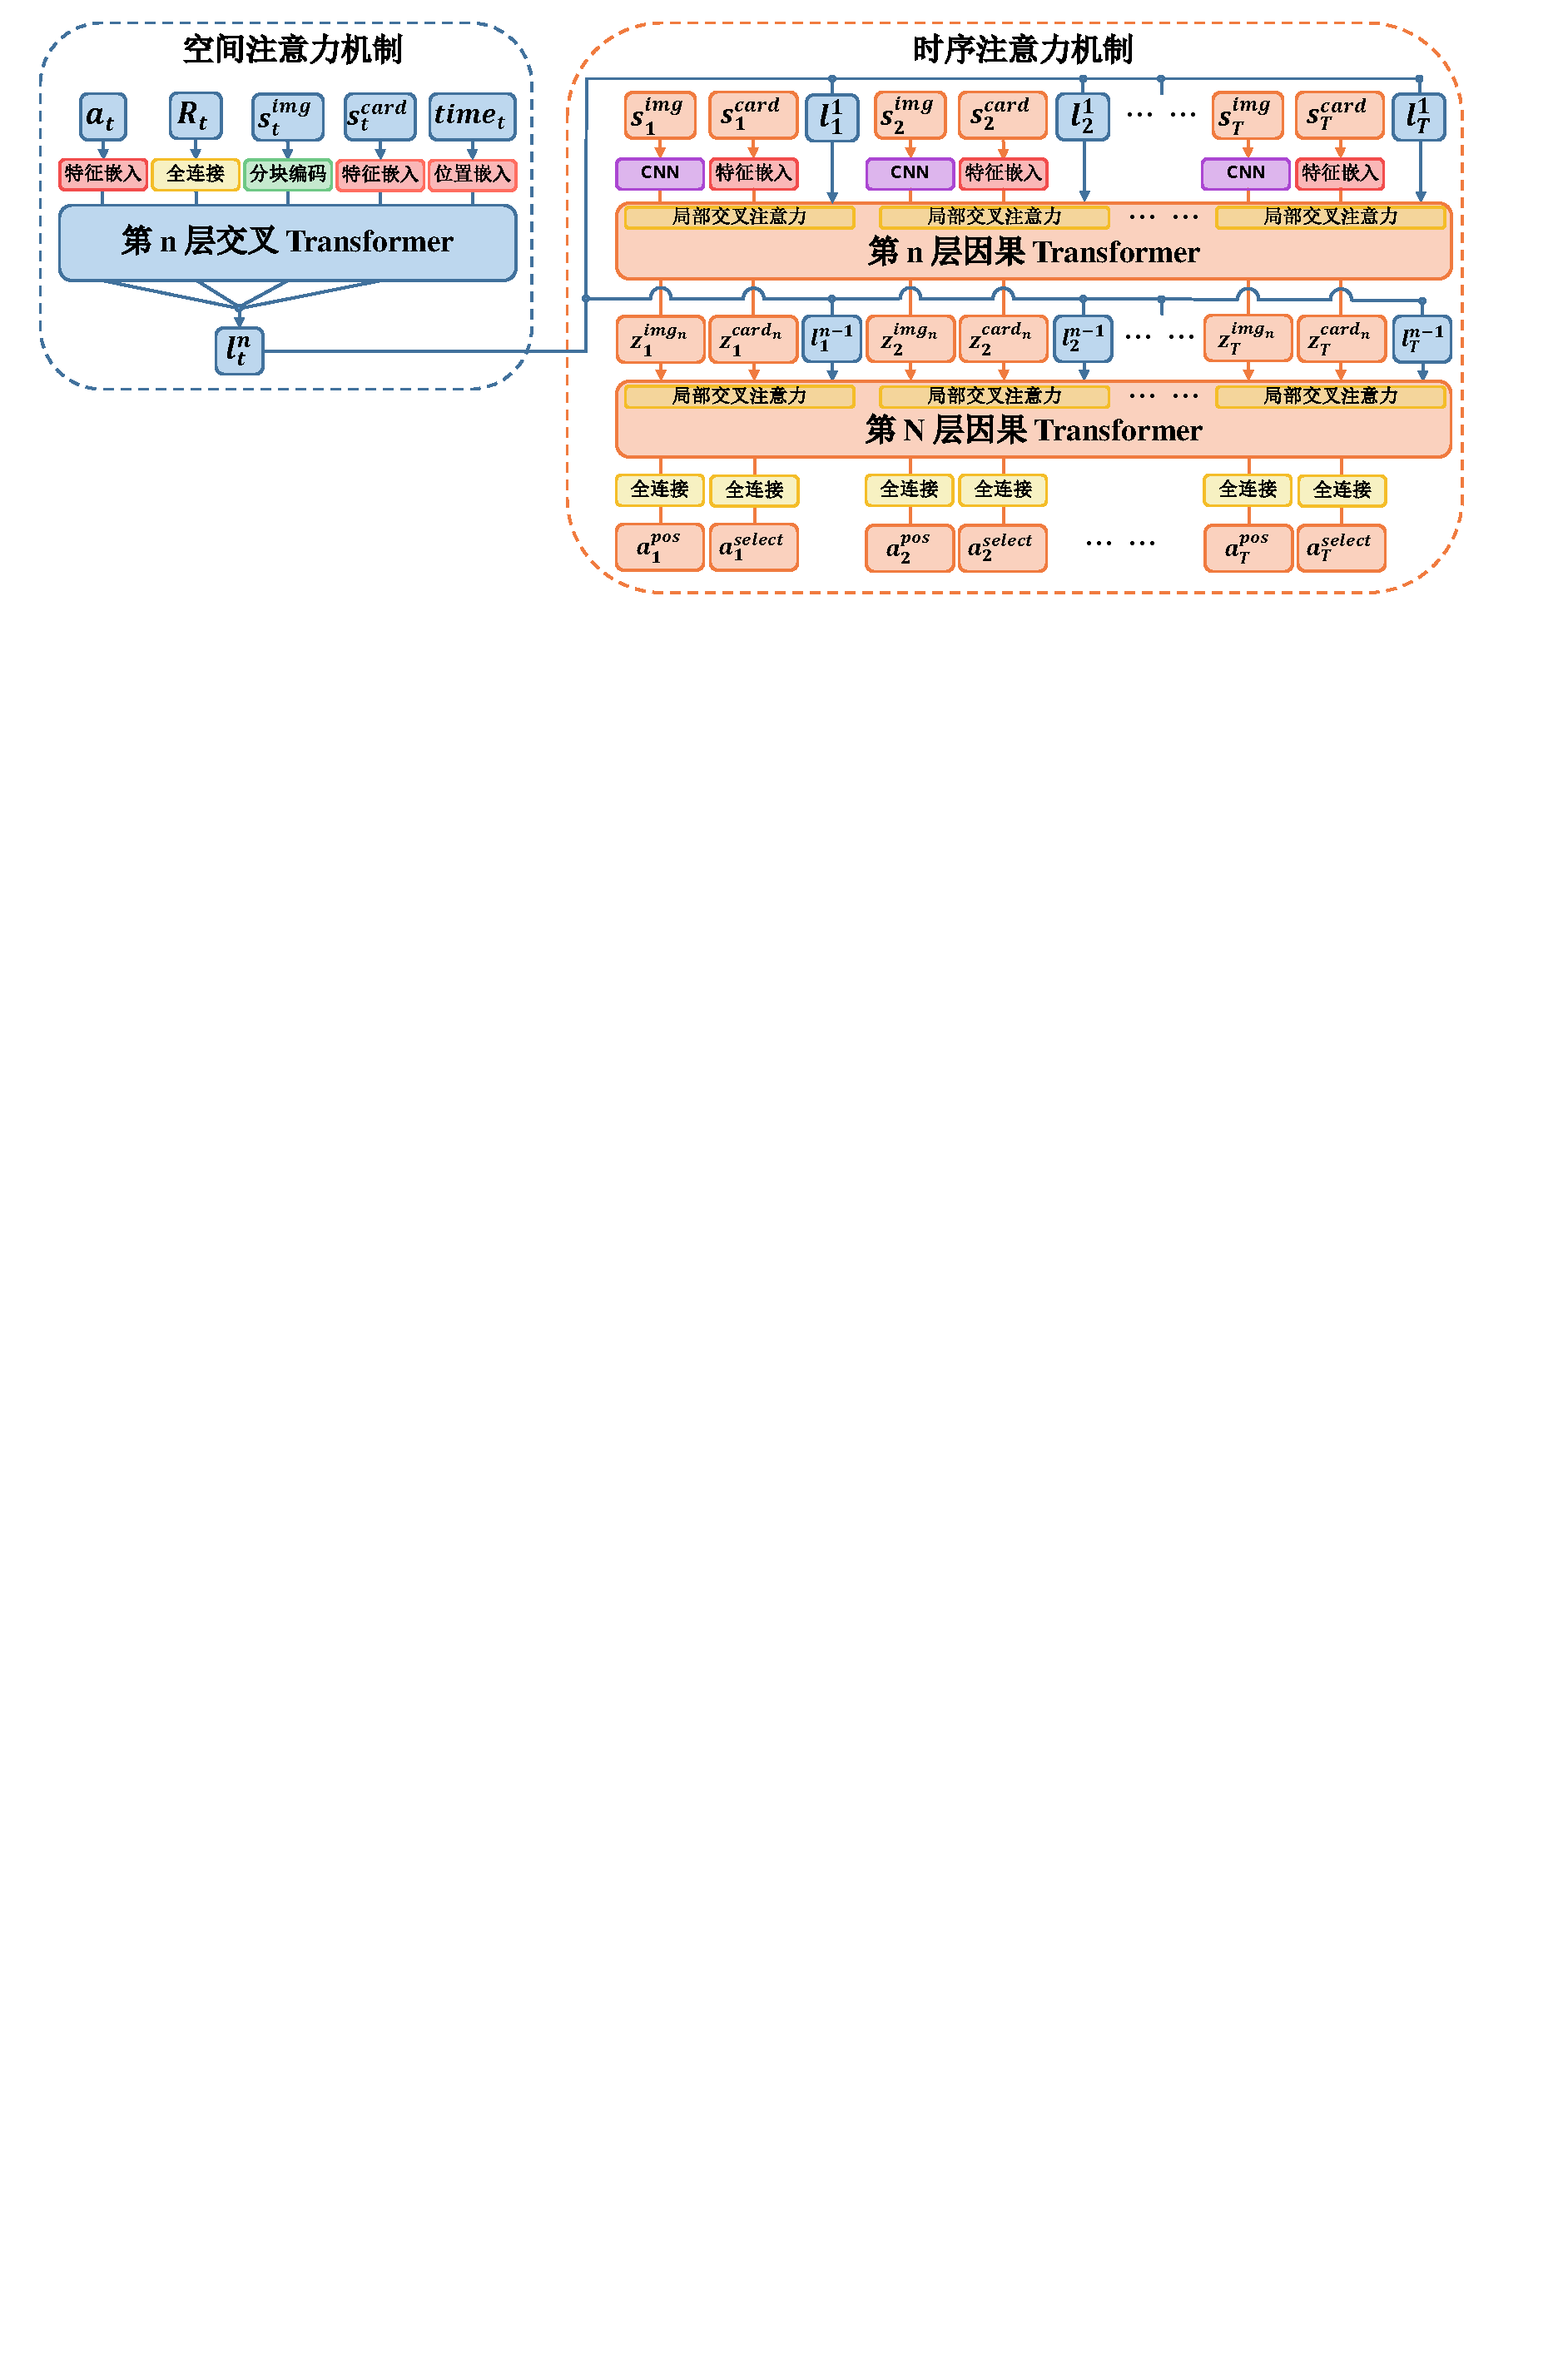
\includegraphics[width=\textwidth]{policy_model.pdf}
  \caption{决策模型:基于StARformer的ViT+DT架构,模型输入为轨迹序列$(a_t, R_t, s_t)_{t=1}^T$,
  输出为动作预测序列$(a_t^{pos},a_t^{select})_{t=1}^T$。左侧交叉注意力机制对
  局部信息$(a_t,R_t,s_t)$按空间维度进行编码,并使用ViT中分块思路将图像$s_t^{img}$转化为序列;
  右侧为因果注意力机制对全局信息$(s^{img}_t,s^{card}_t)$按时序维度进行编码,
  并在每层序列输入中引入对应的局部编码信息$l_t^{n}$。}
  \label{fig-model}
\end{figure}  % 正文
% !Mode:: "TeX:UTF-8" 

\BiChapter{数据分析及实验结果}{5}\label{sec-5}
本章对前3章内容的实验结果进行总结,分别包含第~\ref{chpt-2}~章的生成式数据集分析统计,\ref{sec-perceptron}~的目标识别模型对比实验以及
\ref{sec-model}~的决策模型对比实验。

\BiSection{生成式数据集分析}{}\label{sec-exp-data}
数据集总共分为两部分\footnote{上述数据集统计信息截止于2024年5月6日,全部图像数据集均已开源:
\url{https://github.com/wty-yy/Clash-Royale-Detection-Dataset}}:
\begin{enumerate}
  \item 生成式数据集切片:总计$154$个类别,待识别类别$150$个,总共包含$4654$个切片,
  在全部待识别类别的切片图像中,切片大小分布如图~\ref{fig-segment}~所示。
  \item 目标识别验证集:总计$6939$张人工标记的目标识别图像,包含$116878$个目标框,平均每张图片包含17个目标框,该数据集均为真实对局视频流逐帧标记得到,
  而模型训练所使用的完全是生成式数据集,所以该数据集可以做验证集使用。
\end{enumerate}

\begin{figure}[htbp]
  \centering
  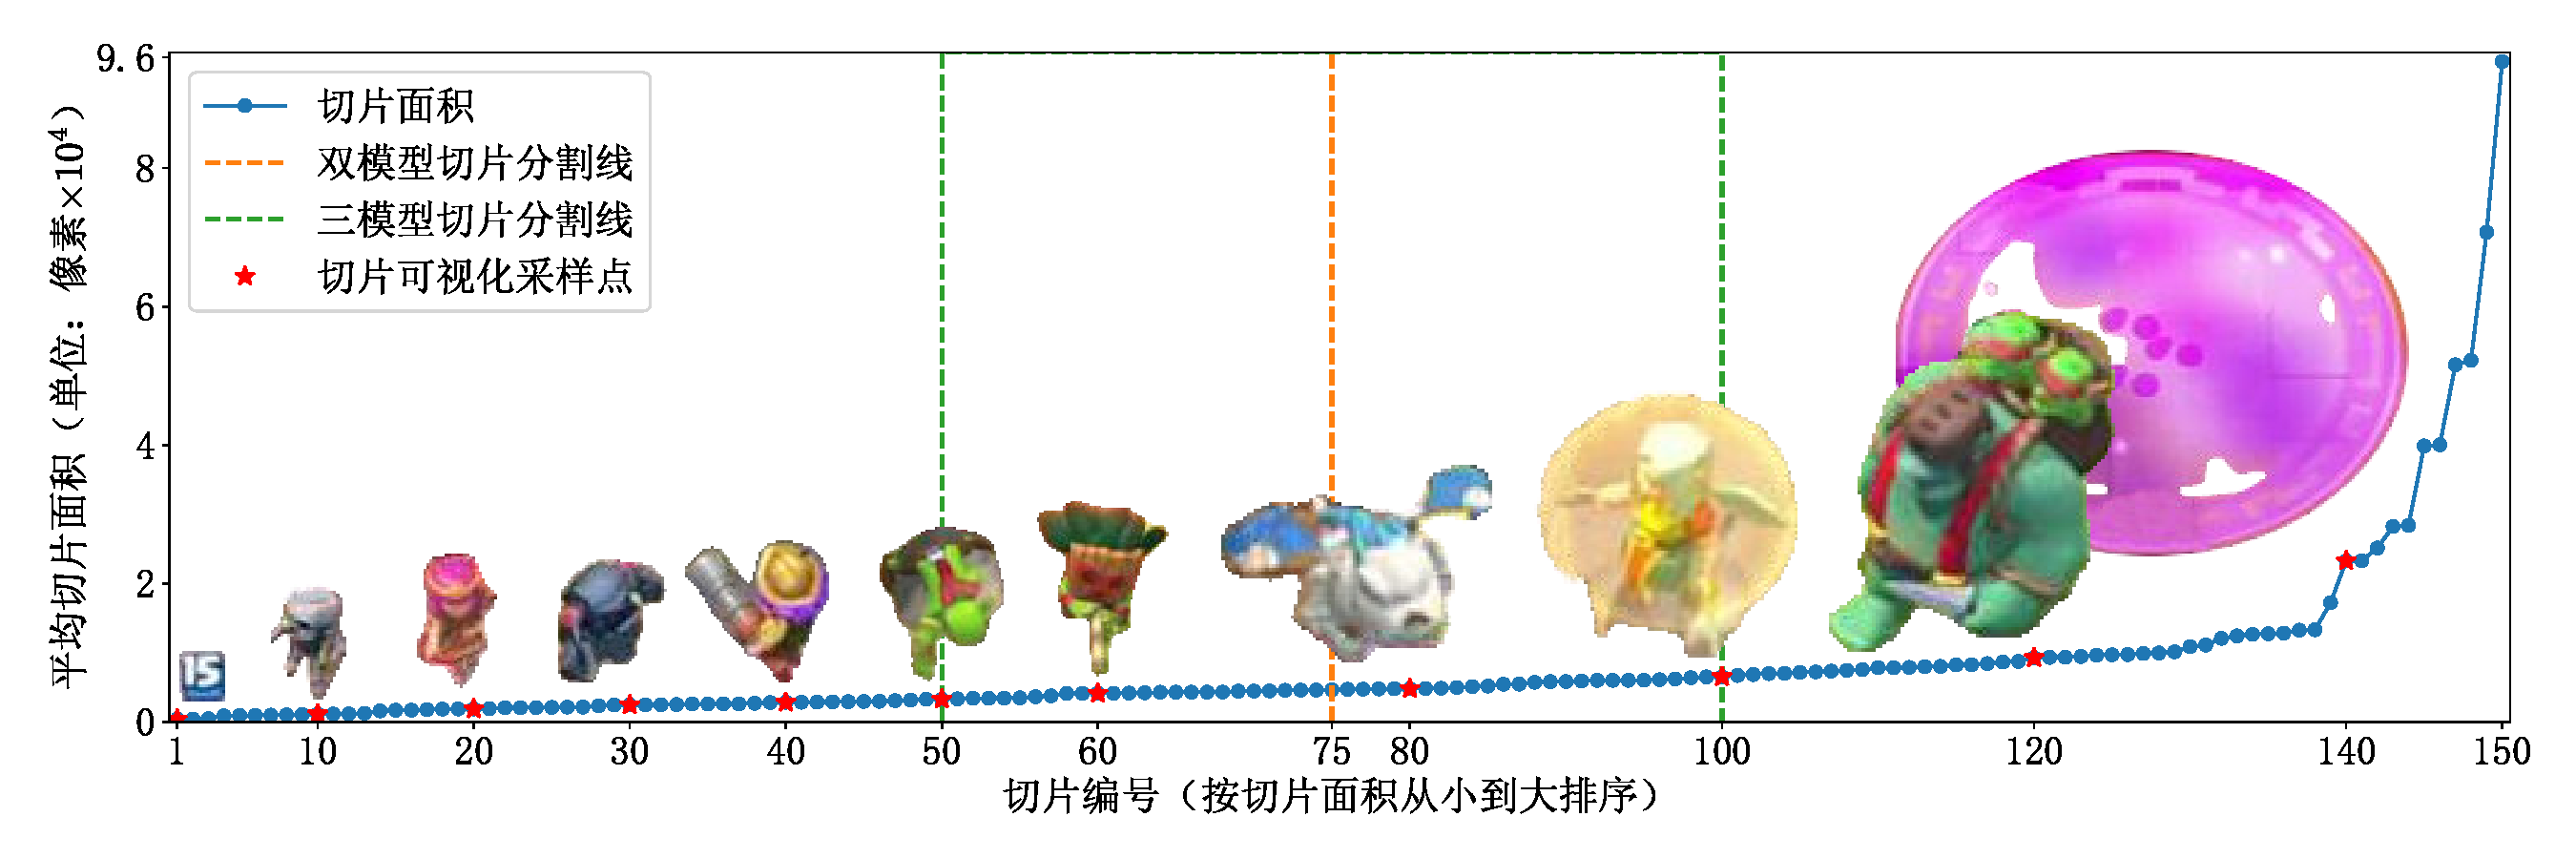
\includegraphics[width=\textwidth]{segment_size.pdf}
  \caption{将切片数据集全部切片按平均面积从小到大排序并编号,
  从中随机采样出部分切片进行可视化。
  分别以全体切片面积的二等分和三等分点,作为双模型和三模型的识别类别分割线。
  }
  \label{fig-segment}
\end{figure}

\BiSection{目标识别模型}{}\label{sec-exp-detect}
目标识别模型使用了自己实现的YOLOv5\footnote{复现YOLOv5代码:\url{https://github.com/wty-yy/KataCV/tree/master/katacv/yolov5}}
和重构后的YOLOv8的模型\footnote{YOLOv8重构内容:\url{https://github.com/wty-yy/KataCR/blob/master/asserts/yolov8_modify.md}},
每个训练集大小设置为$20000$,至多训练$80$个epoch收敛。
数据增强使用了:HSV增强,图像旋转,横纵向随机平移,图像缩放,图像左右反转,具体参数见附录表~\ref{table-app-aug}~。

实验结果\footnote{YOLOv5全部训练曲线:\url{https://wandb.ai/wty-yy/ClashRoyale},YOLOv8全部训练曲线:\url{https://wandb.ai/wty-yy/YOLOv8}}如表~\ref{tabel-yolo}~所示,表中具体内容解释如下:

1. 模型名称:编号后的字母表示模型大小,l,x分别对应大与特大型模型,
YOLOv8-l$\times n$表示使用$n$个YOLOv8-l模型,每个子模型分别识别图~\ref{fig-segment}~中分割线所划分区域中的切片类型,
最后将识别的预测框通过非最大值抑制(Non-Maximum Suppression,NMS)进行筛选,NMS过程中IOU阈值设定为0.6。

2. 评测指标:表中mAP评测指标表示COCO mAP指标\upcite{COCO},即在10种不同IOU阈值下计算PR曲线下面积求平均得到,
AP50、P50、R50和mAP(S)分别表示在判断正例的IOU阈值为$50\%$下的mAP、平均精度、平均召回率和小目标的mAP。

3. 验证速度:模型预测时Batch大小设置为$1$,FPS为模型在GeForce RTX 4090下测试的验证速度,验证测试时置信度设置为$0.001$。
当对视频流数据进行预测时,将置信度改为$0.1$,并使用ByteTrack\upcite{ByteTrack}算法在目标追踪计算过程中对边界框进行筛选,
FPS(T)是在GeForce RTX 4060 Laptop下带有目标追踪的识别速度。

从实验结果可以看出,YOLOv8-l的双识别器对小目标的识别能力与三识别器效果基本一致,并远高出非组合式的识别器,
其原因可能在于$150$个预测类别大小远超模型的识别能力范围,
最大目标与最小目标的边界框大小差距甚远,又由于YOLOv8是无锚框识别头,
由于大目标易于识别,可能导致预测的目标框均偏大,所以多个识别器降低平均类别数能够有效对小目标进行识别。

\begin{table}[!h]
	\renewcommand{\arraystretch}{1.2}
	\centering\wuhao
	\caption{YOLO模型对比测试结果} \label{tabel-yolo} \vspace{2mm}
	\begin{tabularx}{\textwidth} { 
   >{\centering\arraybackslash}X 
   >{\centering\arraybackslash\hsize=.3\hsize}X
   >{\centering\arraybackslash\hsize=.2\hsize}X
   >{\centering\arraybackslash\hsize=.2\hsize}X
   >{\centering\arraybackslash\hsize=.3\hsize}X
   >{\centering\arraybackslash\hsize=.4\hsize}X
   >{\centering\arraybackslash\hsize=.3\hsize}X
   >{\centering\arraybackslash\hsize=.4\hsize}X
   >{\centering\arraybackslash\hsize=.9\hsize}X 
   >{\centering\arraybackslash\hsize=.7\hsize}X
  }
	% \toprule[1.5pt]
  \hline
  模型名称&AP50&P50&R50&mAP&mAP(S)&FPS&FPS(T)&检测器类别数&数据增强\\
  \hline
	% \midrule[1pt]
  YOLOv5-l&66.2&84.4&63.8&53.2&NA&59&NA&151&\\
  YOLOv8-x&83.1&\pmb{93.9}&68.3&67.7&39.8&68&31&160&\\
  YOLOv8-x&\pmb{85.3}&90.7&80.4&66.8&35.9&68&31&160&\checkmark\\
  YOLOv8-l~$\times 2$&84.3&89.5&79.8&67.4&43.9&34&18&85&\checkmark\\
  YOLOv8-l~$\times 3$&85.2&89.7&\pmb{80.9}&\pmb{68.8}&\pmb{48.3}&23&10&65&\checkmark\\
  \hline
	% \bottomrule[1.5pt]
	\end{tabularx}
\end{table}

\BiSection{决策模型}{}\label{sec-decision-model}
本文基于第~\ref{chpt-3}~章中介绍的感知融合技术,
手动构建了玩家与与游戏内置的$8000$分AI对局$105$回合的专家数据
\footnote{全部专家数据集均已开源:\url{https://github.com/wty-yy/Clash-Royale-Replay-Dataset}},
固定双方使用的卡组(具体卡组见附录~\ref{app-sec-desk}~),
数据集总计$113981$帧,动作帧占比$4.01\%$,重采样频次比率为$\frac{\text{动作帧}}{\text{非动作帧}}=24.92:1.04$,
平均动作延迟大小为$21.26$,最大间隔帧数阈值为$T_{delay}=20$(重采样细节见~\ref{sec-target})。
模型损失函数分为三个部分,由于均为离散动作,所以损失函数均使用目标动作均使用交叉熵损失,总损失函数如下
\begin{equation}
  \mathcal{L} =
  \sum_{\substack{i=1\\}}^N\mathbb{I}_{a_i^{delay} < T_{delay}}\left[\mathcal{L}_{\text{CE}}(\hat{\bd{a}}_i^{pos}, \bd{a}_i^{pos})+
  \mathcal{L}_{\text{CE}}(\hat{a}_i^{select}, a_i^{select}) + 
  \mathcal{L}_{\text{CE}}(\hat{a}_i^{delay}, a_i^{delay})\right]
\end{equation}
其中$T_{delay},\bd{a}_i^{pos},a_i^{select},a_i^{delay}$分别为最大间隔帧数阈值、目标动作的部署坐标、手牌编号以及部署延迟,
注意每条轨迹下只考虑$a_i^{delay} < T_{delay}$对应的梯度。

本文分别测试了下述模型参数:
\begin{itemize}
  \item 不同的模型架构(架构设计见~\ref{sec-model}~),分别测试了StARformer和DT架构。
  \item 模型输入的轨迹步长记为$L$,测试了$L=30,50,100$的情况。
  \item 不同的预测目标(离散与连续预测见~\ref{sec-target}~)。
  \item 不同的手牌预测范围,默认预测当前手牌编号,也尝试了对当前牌库中全部手牌进行预测。
\end{itemize}

本文使用了如下数据增强方式对模型进行训练:
\begin{itemize}
  \item 重采样:对稀疏的动作帧按比例进行进行重采样,加快模型收敛,缓解离线数据集的长尾问题。
  \item 随机手牌重组:对当前输入轨迹中的全部手牌按照随机排列进行打乱,当预测全部手牌编号时,将动作对应的手牌也进行相应变换。
\end{itemize}

全部模型训练曲线均进行了上传\footnote{决策模型全部训练曲线:\url{https://wandb.ai/wty-yy/ClashRoyale\%20Policy}},
模型实时对局的验证结果总结于表\ref{table-model-eval}中,在实时对局的实现中包含以下细节:
\begin{itemize}
  \item 动作执行:对于连续动作预测模型中,由于感知识别中存在延迟,当预测动作延迟在$8$帧以内就会立刻执行动作,
  并且为了避免总圣水溢出导致的惩罚奖励,每当总圣水达到$10$时就直接下出当前预测的卡牌。
  \item 无效动作跳过:若模型预测出的卡牌所需圣水超出了当前总圣水量或当前动作执行的卡牌位为空。
\end{itemize}

\begin{table}[!h]
	\renewcommand{\arraystretch}{1.2}
	\centering\small
  %\wuhao
	\caption{决策模型对比}\label{table-model-eval}\vspace{2mm}
	\begin{tabularx}{\textwidth} { 
   >{\centering\arraybackslash\hsize=1.4\hsize}X 
   >{\centering\arraybackslash\hsize=0.6\hsize}X 
   >{\centering\arraybackslash}X 
   >{\centering\arraybackslash}X
   >{\centering\arraybackslash}X
   >{\centering\arraybackslash}X 
   >{\centering\arraybackslash}X 
   >{\centering\arraybackslash\hsize=.5\hsize}X
   }
	\toprule[1.5pt]
	模型框架&步长$L$&训练回合&总奖励&对局时长/秒&动作数&胜率\\
	\midrule[1pt]
  DT-4L&$50$&$8$&$-5.7\pm 2.5$&$148.9\pm 33.6$&$128.7\pm 37.7$&$5\%$\\
  StARformer-2L&$30$&$3$&$-6.0\pm 2.3$&$135.0\pm 35.1$&$141.8\pm 57.9$&$5\%$\\
  StARformer-2L&$50$&$8$&$-6.2\pm 2.2$&$131.9\pm 44.3$&$195.3\pm 69.8$&$5\%$\\
  StARformer-2L&$100$&$1$&$-4.9\pm 2.8$&$150.2\pm 35.6$&$187.6\pm 48.2$&$0\%$\\
  StARformer-3L&$30$&$4$&$-5.1\pm 3.7$&$147.2\pm 37.4$&$190.8\pm 52.7$&\pmb{$10\%$}\\
  StARformer-3L&$50$&$3$&\pmb{$-4.7\pm 3.1$}&\pmb{$158.9\pm 27.7$}&\pmb{$207.8\pm 48.2$}&$5\%$\\
  StARformer-3L&$100$&$5$&$-6.1\pm 2.2$&$125.9\pm 37.8$&$144.6\pm 42.9$&$5\%$\\
  \makecell[c]{StARformer-3L\\[-1ex](全卡牌预测)}&$50$&$2$&$-5.6\pm 2.1$&$150.2\pm 38.6$&$195.3\pm 69.8$&$0\%$\\
  \makecell[c]{StARformer-2L\\[-1ex](离散动作预测)}&$50$&$1$&$-7.5\pm 0.8$&$123.1\pm 39.2$&$21.9\pm 9.4$&$0\%$\\
	\bottomrule[1.5pt]
	\end{tabularx}
\end{table}

表~\ref{table-model-eval}~中记录了为每个模型的前10次训练结果中,与环境交互20个回合得到的最高平均奖励,
从中可以看出,将离散预测改为连续预测提高了$37\%$的性能、StARformer架构从2L修改为3L的改动提高了$24\%$的模型性能。
表中每列的含义分别为:
\begin{itemize}
  \item 步长$L$:为模型架构设计~\ref{sec-model-struct}~中的输入轨迹长度。
  \item 训练回合:前10个训练结果中,获得最高奖励所对应的回合数。
  \item 总奖励:按奖励公式~(\ref{eq-reward})~进行累计得到的总奖励。
  \item 对局时长:统计每次对局的时长。
  \item 动作数:统计每局智能体成功执行的动作数目。
  \item 胜率:按照~\ref{game-target}~中介绍的游戏目标,判定智能体的获胜概率。
\end{itemize}


硬件交互方法见附录~\ref{app-interaction},本文使用的验证环境:手机系统为鸿蒙、电脑系统为Ubuntu24.04 LTS、CPU: R9 7940H、GPU: RTX GeForce 4060 Laptop,
平均决策用时120ms,感知融合用时240ms。

图~\ref{fig-model-eval}~中展示了每种模型前10个训练结果的验证曲线。

\begin{figure}[h!]
  \centering
  \subfigure[不同模型结构]{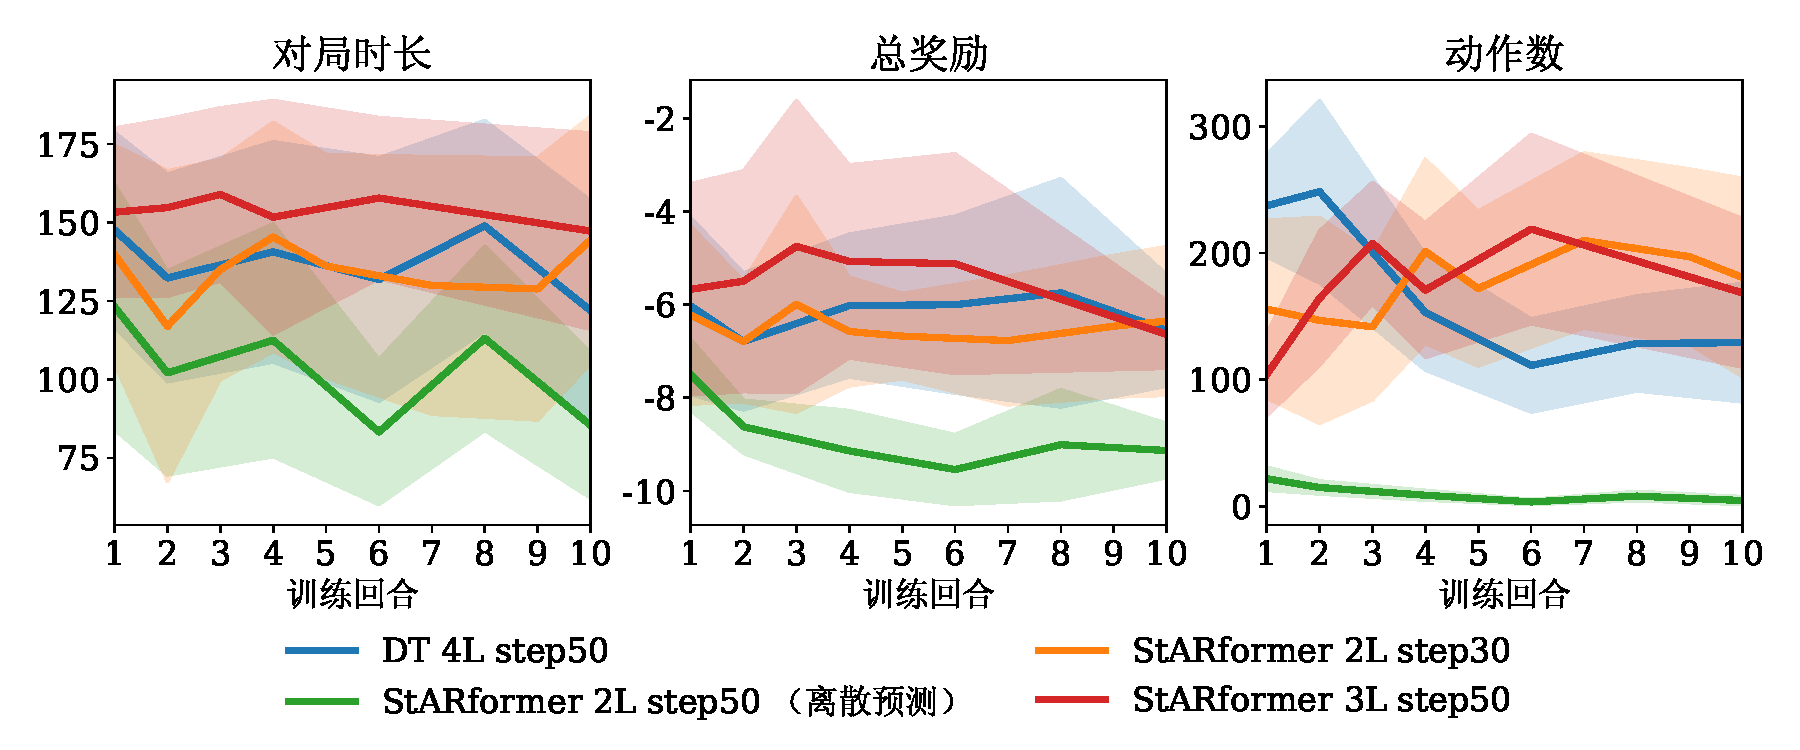
\includegraphics[width=\textwidth]{diff_model.pdf}}
  \subfigure[StARformer-3L采取不同轨迹长度]{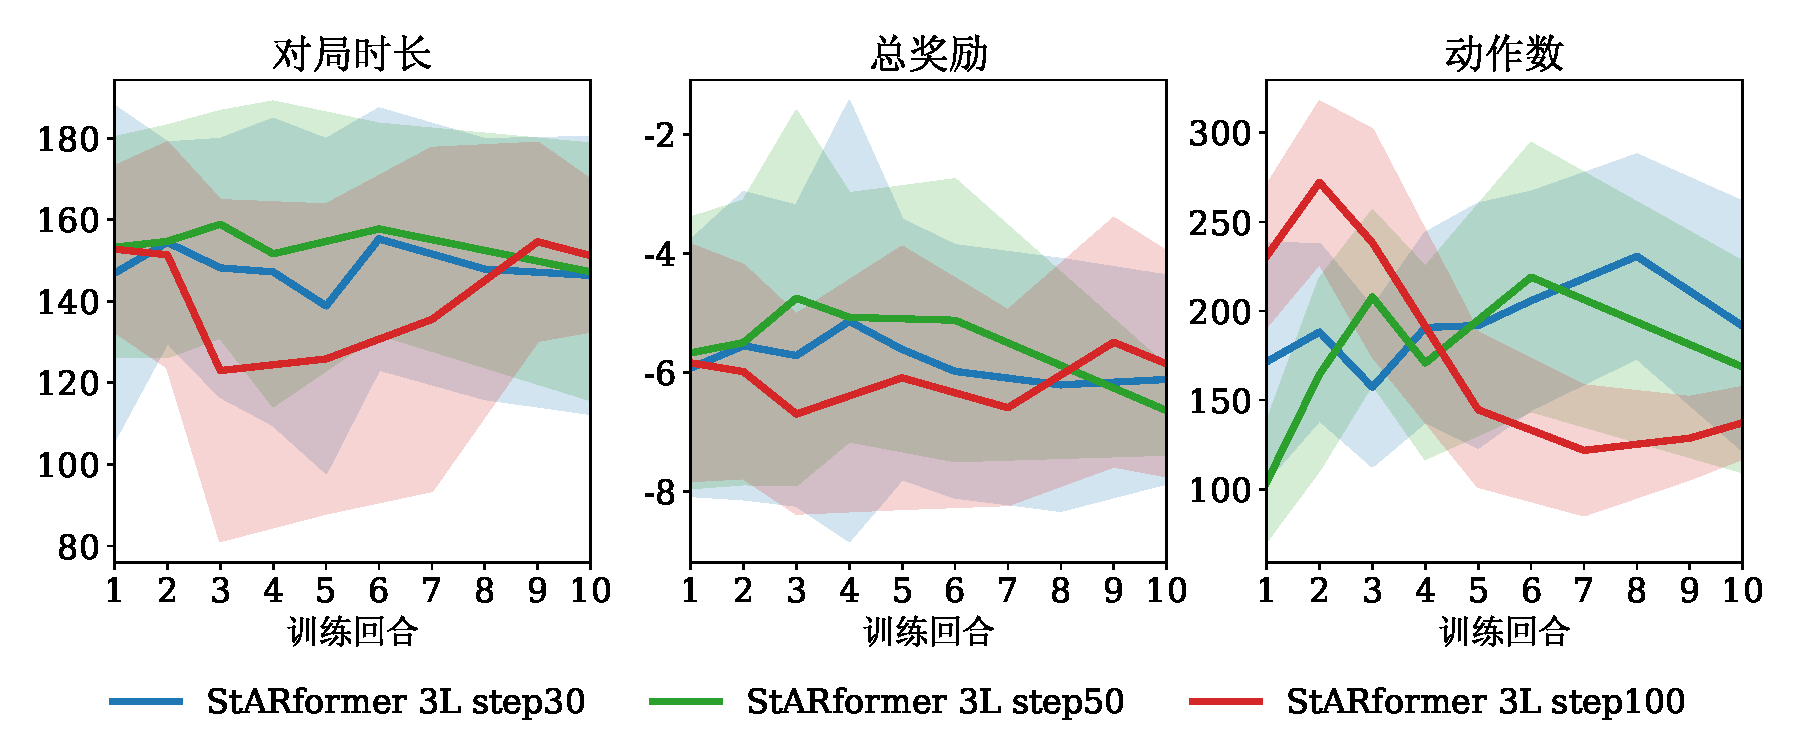
\includegraphics[width=\textwidth]{diff_3L_nstep.pdf}}
  \setlength{\abovecaptionskip}{0ex}  % 由于minted会增大图像与标题间距需要进行缩小
  \caption{模型验证曲线:展示了前10个训练结果,每回合模型在真实对局中的对局时间时长、总奖励和执行动作数,
  每次进行20次对局,实线为均值、虚影为标准差。}\label{fig-model-eval}
\end{figure}
  % 正文
% !Mode:: "TeX:UTF-8" 

\BiChapter{总结与展望}{6}

% 本文首次提出了一种基于非嵌入式离线强化学习的训练策略,应用于游戏皇室战争(Clash Royale)。
% 结合当前目标识别与光学文本识别的顶尖算法,使用离线强化学习算法制定策略,成功实现了智能体在非嵌入条件下的实时对局:
% 移动设备上实时图像获取、感知融合、智能模型决策及控制移动设备执行动作,从而能够与对手进行实时对局,并且能够战胜游戏中的内置AI。
% 
% 首先,本文设计了一种高效制作切片数据集的方法,基于该方法制作了包含$4654$张切片、共150个类别的切片数据集,
% 以及包含$116878$个目标框、共$6939$张图像的目标识别数据集\footnote{图像数据集:\url{https://github.com/wty-yy/Clash-Royale-Detection-Dataset}\hfill},
% 并提出了一种可行的生成式目标识别数据集算法,使其能够模拟真实对局场景生成含有任意数量部队及种类的带标签图像。
% 通过生成式图像训练出的模型在真实视频流中表现出良好的泛化性,具有很高的识别准确率。
% 
% 其次,本文基于计算机视觉模型的输出结果设计了感知融合算法,该算法结合视频数据中的上下帧信息优化特征结果,从而进一步提升识别的准确率。
% 
% 最后,在决策模型方面,本文从架构及预测目标两个方面对传统模型进行了改进,将难以学习的离散动作序列转化为连续动作序列,
% 大幅提高了模型性能。本文制作了包含$105$回合、总共$113981$帧的专家数据集\footnote{专家数据集:\url{https://github.com/wty-yy/Clash-Royale-Replay-Dataset}\hfill},
% 并基于该离线数据集在不与真实环境交互的条件下,训练出了能够战胜游戏内置AI的智能体。
% 
\BiSection{结论}{}
本文基于游戏皇室战争(Clash Royale),首次提出了一种基于非嵌入式的离线强化学习训练策略。
结合目标识别和光学文本识别的顶尖算法,成功实现了智能体在移动设备上进行实时对局,并且战胜了游戏中的内置AI。

主要贡献包含以下三点:
\begin{enumerate}
  \item 数据集制作:本文设计了一种高效制作切片数据集的方法,制作了包含4654张切片、共150个类别的切片数据集,
  以及包含116878个目标框、共6939张图像的目标识别数据集。提出的生成式目标识别数据集算法可以模拟真实对局场景生成带标签的图像,
  通过生成式图像训练的模型在真实视频流中表现出良好的泛化性,具有很高的识别准确率。
  \item 图像感知融合算法:基于计算机视觉模型的输出结果,设计了图像感知融合算法,该算法结合视频数据中的上下帧信息优化特征结果,进一步提升了识别的准确率。
  \item 决策模型改进:在决策模型方面,从架构及预测目标两个方面对传统模型进行改进,
  将难以学习的离散动作序列转化为连续动作序列,大幅提高了模型性能。制作了包含105回合、总共113981帧的专家数据集,并基于该离线数据集训练出能够战胜游戏内置AI的智能体。
\end{enumerate}

\BiSection{展望}{}
本文为非嵌入式强化学习在移动设备上的应用提供了新的思路。未来的工作可以从以下几个方面进行扩展:
\begin{enumerate}
  \item 数据集的扩展与优化:增加数据集的规模和多样性,进一步提升模型的泛化能力和识别准确率。
  \item 算法的改进:当前在固定卡组下进行训练,仍然无法$100\%$战胜游戏中的内置AI,因此远无法达到人类平均水平,
  而且制作离线强化学习数据集需要花费大量的人力,
  若要进一步提升智能体能力,应该需要采用在线强化学习算法,与此同时需要使用更加高效的图像感知融合算法和决策模型架构,才有可能进一步提高智能体的实时决策能力和对局胜率。
  \item 实际应用的拓展:将本文的方法应用于更多的游戏和实际场景中,验证其通用性和实用价值。
\end{enumerate}

本文的全部代码均已开源\footnote{全部代码:\url{https://github.com/wty-yy/katacr}},期望能够为相关领域的研究者提供有价值的参考和借鉴。  % 正文
\documentclass{article}
\usepackage{tabularx}
\usepackage{array}

\begin{document}
\begin{table}[!h]
	\centering
	\caption{YOLO} \label{tabel-yolo} \vspace{2mm}
	\begin{tabularx}{\textwidth} { 
   >{\centering\arraybackslash}X 
   >{\centering\arraybackslash\hsize=.4\hsize}X
   >{\centering\arraybackslash\hsize=.4\hsize}X
   >{\centering\arraybackslash\hsize=.4\hsize}X
   >{\centering\arraybackslash\hsize=.4\hsize}X
   >{\centering\arraybackslash}X 
   >{\centering\arraybackslash}X 
   >{\centering\arraybackslash\hsize=.7\hsize}X
  }
	\hline
  a&mAP&AP50&P50&R50&bmAP&c&d\\
	\hline
  YOLOv8&\textbf{68.8}&85.2&89.7&\underline{80.9}&\underline{48.3}&65&e\\
	\hline
	\end{tabularx}
\end{table}
\end{document}
  % 正文
% !Mode:: "TeX:UTF-8" 

\BiAppendixChapter{致\quad 谢}{Acknowledgements}

感谢西安交通大学数学学院能够给我这次自拟毕设题目的机会,如果错过这次机会,之后可能很难再有充足的时间与精力完成本毕设内容;
感谢数学学院强基计划,通过本科课程学习,使我有了扎实的数学基础,能够比较轻松地看懂计算机视觉、强化学习等领域中的论文,
理解并对其中的公式进行推导加深理解,最后使用代码进行复现。

感谢兰旭光老师对本毕设的支持,即使本毕设内容充满各种未知挑战,但老师仍给我提供了必要的算力支持,如果没有充足算力,本文进展将相当缓慢,完全无法完成任务。
感谢课题组中各位师兄师姐为本次毕设提供思路,其中使用SAM辅助切片制作和多目标识别模型进行目标检测思路来自王宇航博士,
决策模型中将离散预测转化为连续预测思路来自万里鹏博士,如果没有这些改进,精准的识别模型可能无法实现,决策模型也没有任何性能,
战胜游戏中的内置AI成为幻想。还要感谢我身边朋友的支持,他们的支持使我愈发坚定将不可能变为可能的决心。

感谢我的父母对我一直以来的支持,使我能在高中参加算法竞赛,打下扎实的编程基础,
并支持我去追随自己的儿时的梦想——“做出一个能够与现实进行直接交互并改善生活的智能体”。
如果没有这样坚定的梦想,我可能早在制作数据集的枯燥过程中放弃,但通过大学的各种知识与技术的学习,
使我看到了前进的道路,坚定下自己的信念,将全部代码从零实现了出来,从而初步完成了本毕设开题时所设定的目标,也成功地走出了第一步。
  % 致谢

%======================================= Reference =======================================
\wuhao\selectfont
\bibliographystyle{bib/xjtuthesis-numerical}
\addcontentsline{toc}{chapter}{参考文献}
\addcontentsline{toe}{chapter}{References}
\addtolength{\bibsep}{-0.8em}
\bibliography{bib/mybib}
% \begin{thebibliography}{99}
  \bibitem{bib-ref1}Dimitris G M, Vinay K I, Stephen M K. Statistical and adaptive signal processing[M]. Norwood: Artech House, Inc., 2005.
\end{thebibliography}
% \begin{thebibliography}{99}
%   \bibitem{ref1}Dimitris G M, Vinay K I, Stephen M K. Statistical and adaptive signal processing[M]. Norwood: Artech House, Inc., 2005.
% \end{thebibliography}

%======================================= Appendix ========================================
% !Mode:: "TeX:UTF-8" 

\appendix
\defaultfont
\renewcommand{\appendixname}{附录~\Alph{chapter}}
\CTEXsetup[name={附录}]{chapter}

\renewcommand{\thefigure}{\Alph{chapter}-\arabic{figure}}
\renewcommand{\thetable}{\Alph{chapter}-\arabic{table}}
\renewcommand{\theequation}{附录\Alph{chapter}-\arabic{equation}}
% \renewcommand{\thelstlisting}{\Alph{chapter}-\arabic{lstlisting}}

% \setlength{\abovecaptionskip}{0ex}  % 由于minted会增大图像与标题间距需要进行缩小  % 附录配置

\BiAppChapter{外文文献原文}{Translation}

{\centering
\vspace{-5ex}
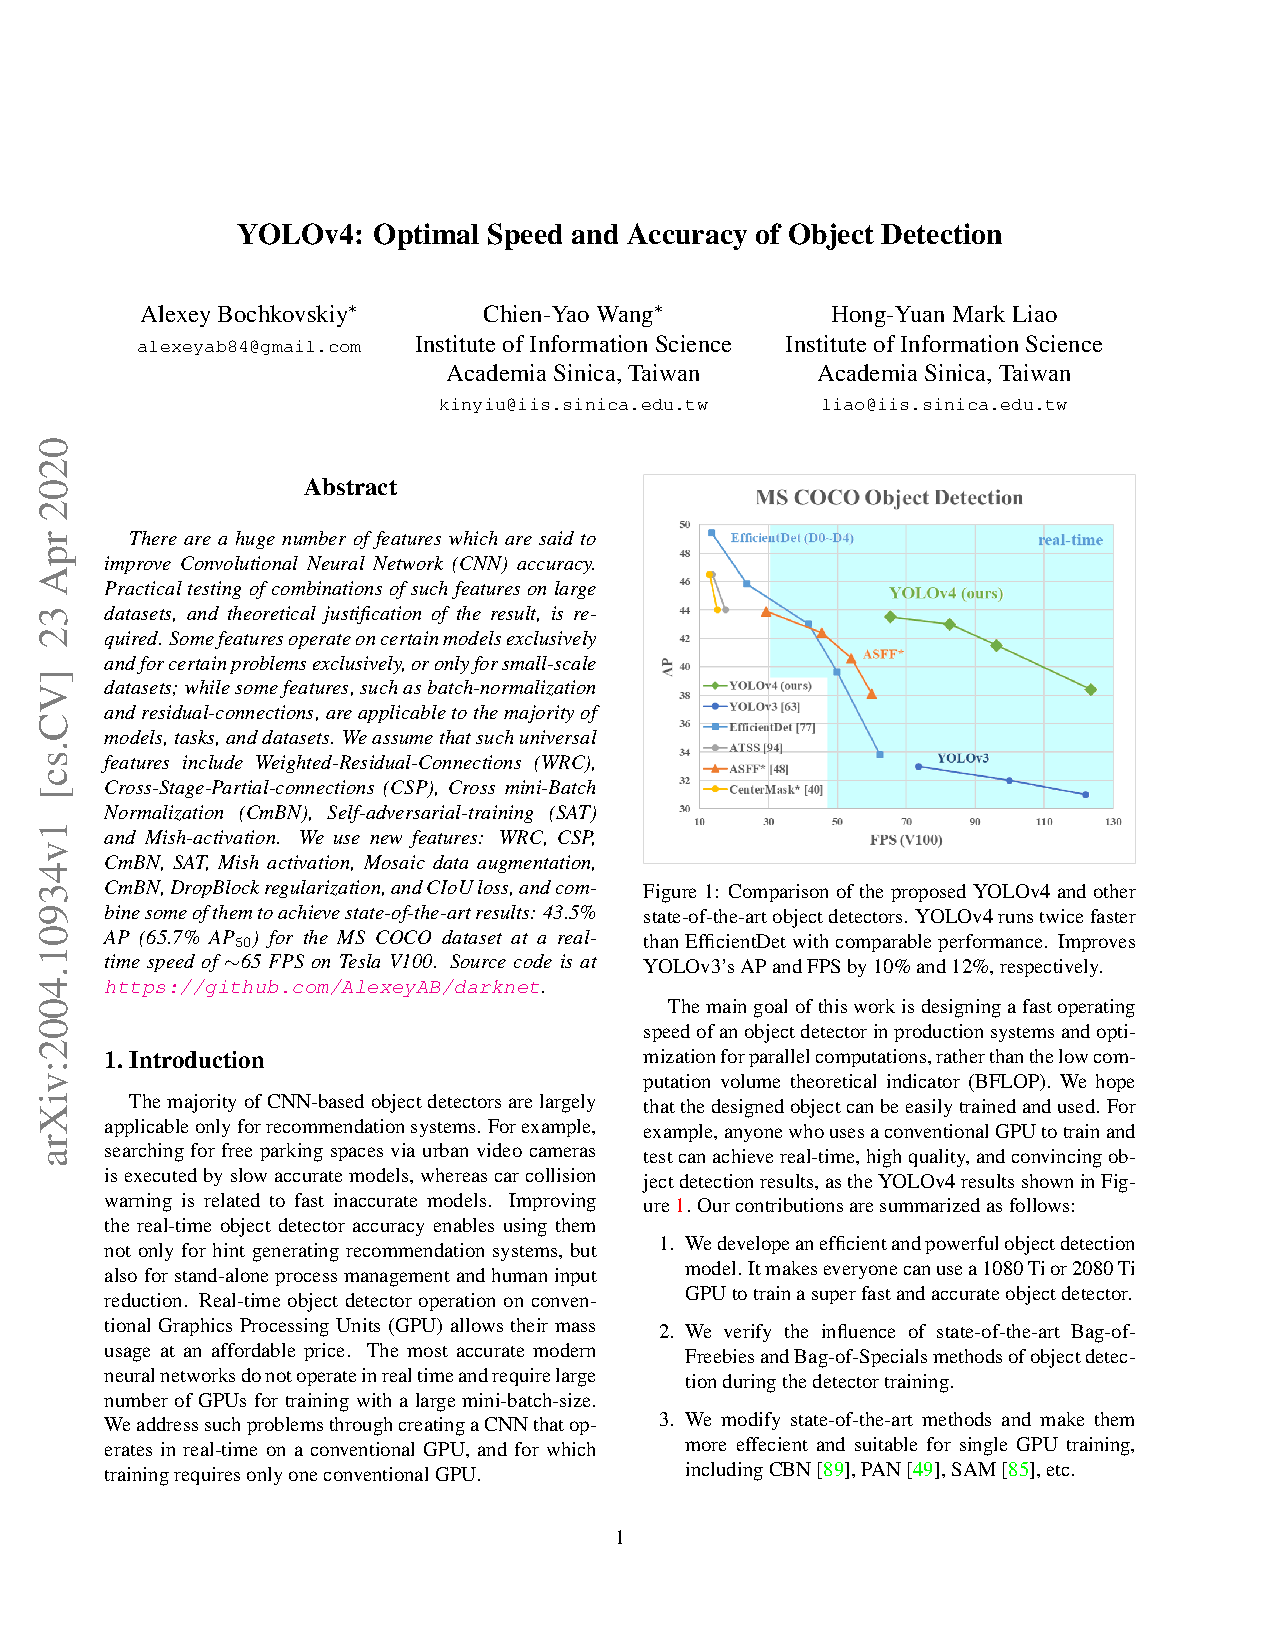
\includegraphics[width=\textwidth, page=1, trim = 15mm 20mm 15mm 20mm]{pdfs/外文翻译YOLOv4原文.pdf}
\includegraphics[width=\textwidth, page=2, trim = 15mm 20mm 15mm 20mm]{pdfs/外文翻译YOLOv4原文.pdf}
\includegraphics[width=\textwidth, page=3, trim = 15mm 20mm 15mm 20mm]{pdfs/外文翻译YOLOv4原文.pdf}
\includegraphics[width=\textwidth, page=4, trim = 15mm 20mm 15mm 20mm]{pdfs/外文翻译YOLOv4原文.pdf}
\includegraphics[width=\textwidth, page=5, trim = 15mm 20mm 15mm 20mm]{pdfs/外文翻译YOLOv4原文.pdf}
\includegraphics[width=\textwidth, page=6, trim = 15mm 20mm 15mm 20mm]{pdfs/外文翻译YOLOv4原文.pdf}
\includegraphics[width=\textwidth, page=7, trim = 15mm 20mm 15mm 20mm]{pdfs/外文翻译YOLOv4原文.pdf}
\includegraphics[width=\textwidth, page=8, trim = 15mm 20mm 15mm 20mm]{pdfs/外文翻译YOLOv4原文.pdf}
\includegraphics[width=\textwidth, page=9, trim = 15mm 20mm 15mm 20mm]{pdfs/外文翻译YOLOv4原文.pdf}
\includegraphics[width=\textwidth, page=10, trim = 15mm 20mm 15mm 20mm]{pdfs/外文翻译YOLOv4原文.pdf}
}

% 外文文献以图片的形式插入,不会发生失真  % 外文原文

\BiAppChapter{外文文献译文}{Translation}

{\centering
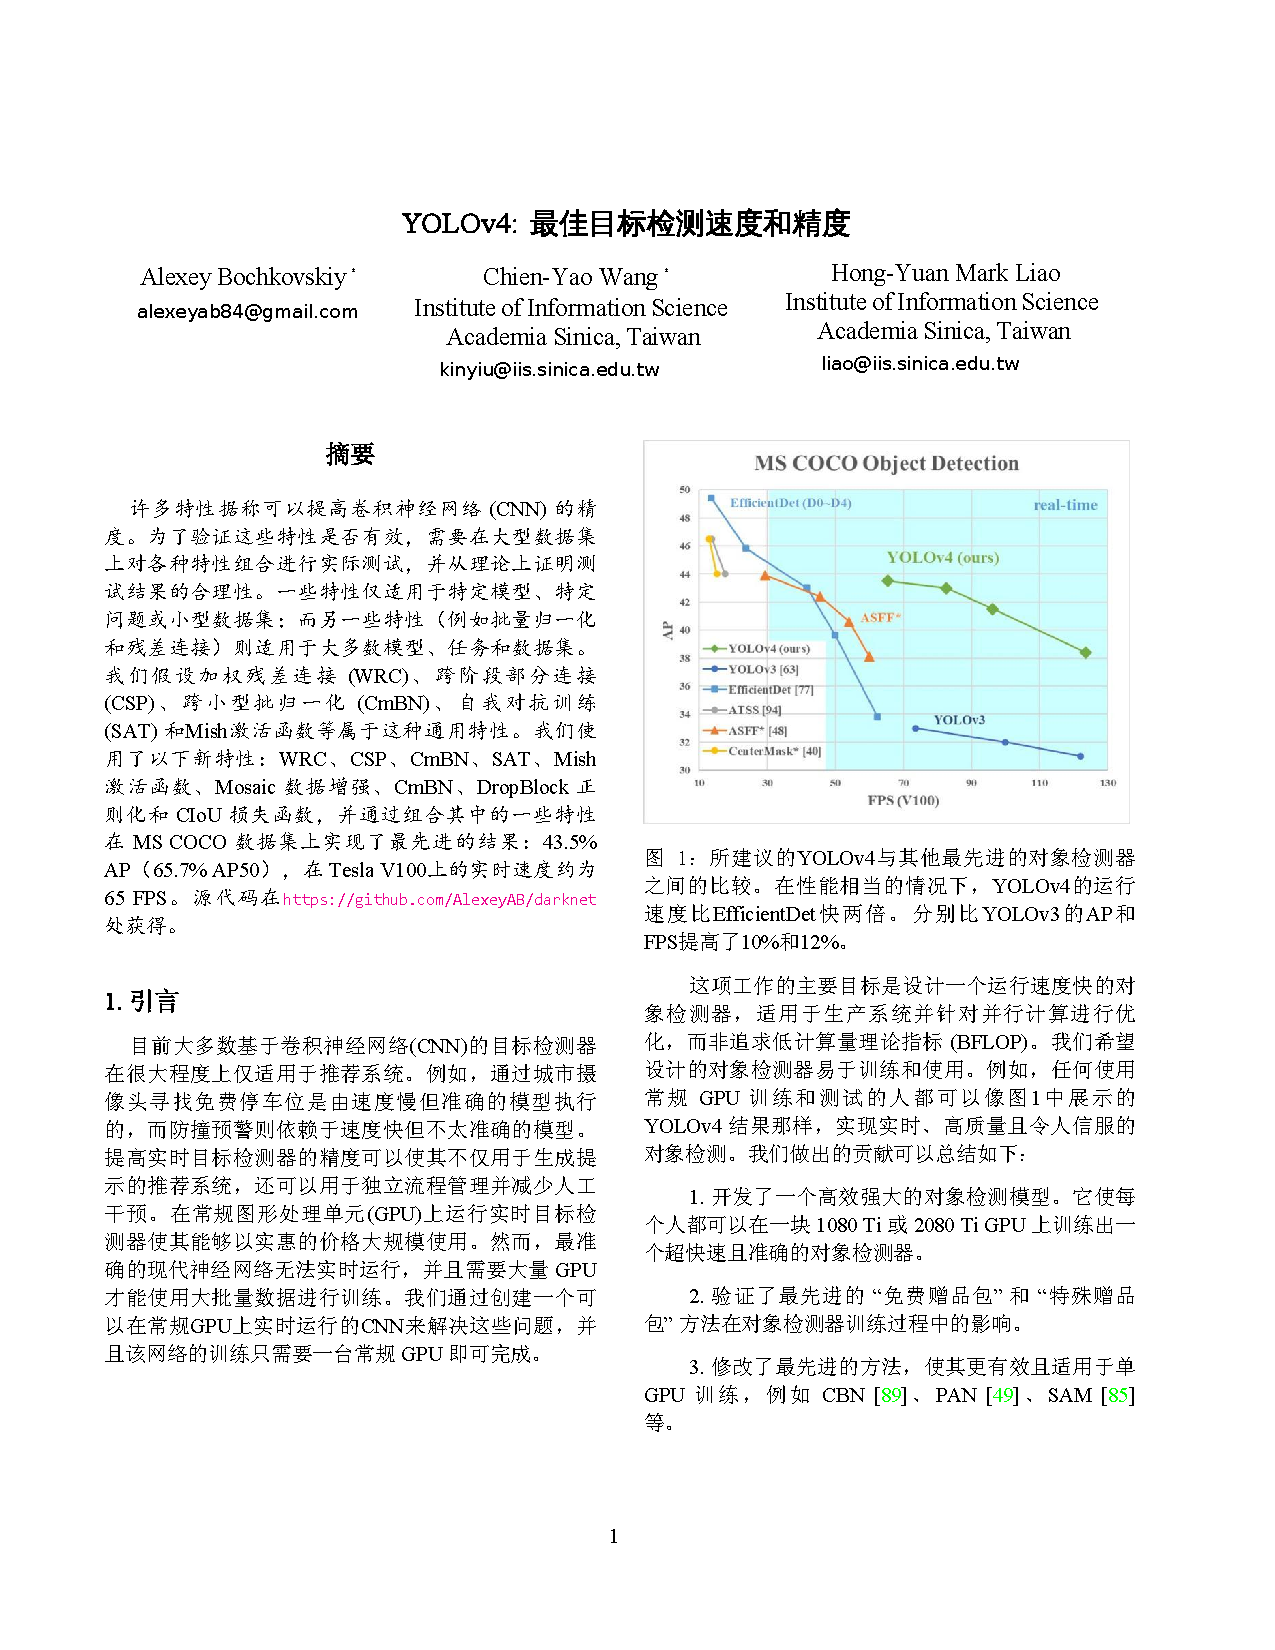
\includegraphics[width=\textwidth, page=1, trim = 15mm 20mm 15mm 20mm]{pdfs/外文翻译YOLOv4译文.pdf}
\includegraphics[width=\textwidth, page=2, trim = 15mm 20mm 15mm 20mm]{pdfs/外文翻译YOLOv4译文.pdf}
\includegraphics[width=\textwidth, page=3, trim = 15mm 20mm 15mm 20mm]{pdfs/外文翻译YOLOv4译文.pdf}
\includegraphics[width=\textwidth, page=4, trim = 15mm 20mm 15mm 20mm]{pdfs/外文翻译YOLOv4译文.pdf}
\includegraphics[width=\textwidth, page=5, trim = 15mm 20mm 15mm 20mm]{pdfs/外文翻译YOLOv4译文.pdf}
\includegraphics[width=\textwidth, page=6, trim = 15mm 20mm 15mm 20mm]{pdfs/外文翻译YOLOv4译文.pdf}
\includegraphics[width=\textwidth, page=7, trim = 15mm 20mm 15mm 20mm]{pdfs/外文翻译YOLOv4译文.pdf}
\includegraphics[width=\textwidth, page=8, trim = 15mm 20mm 15mm 20mm]{pdfs/外文翻译YOLOv4译文.pdf}
\includegraphics[width=\textwidth, page=9, trim = 15mm 20mm 15mm 20mm]{pdfs/外文翻译YOLOv4译文.pdf}
}

% 外文文献以图片的形式插入,不会发生失真  % 外文翻译

\BiAppChapter{外文文献原文}{Translation}

{\centering
\includegraphics[width=\textwidth, page=1, trim = 15mm 20mm 15mm 20mm]{figures/CVPR20c.pdf}

\includegraphics[width=\textwidth, page=2, trim = 15mm 20mm 15mm 20mm]{figures/CVPR20c.pdf}}

% 外文文献以图片的形式插入,不会发生失真  % 附录C
% -*-coding: utf-8 -*-

\BiAppChapter{论文相关代码}{}

本论文全部代码均已开源~\url{https://github.com/wty-yy/katacr}~,核心代码总计1.4万行左右,架构设计如下:

\setitemize{leftmargin=2em,itemsep=0em,partopsep=0em,parsep=0em,topsep=-0em}
\begin{itemize}
  \item \texttt{build\_dataset}
  \begin{itemize}
    \item 对视频文件进行预处理(划分episode,逐帧提取,图像不同部分提取)
    \item 目标识别数据集搭建工具(辅助标记数据集,数据集版本管理,生成式目标识别,标签转化及识别标签生成,图像切片提取)
  \end{itemize}
  \item \texttt{classification}:用ResNet进行手牌及圣水分类
  \item \texttt{constants}:常量存储(卡牌名称及对应圣水花费,目标识别类别名称)
  \item \texttt{detection}:自行用JAX复现的YOLOv5模型(后弃用)
  \item \texttt{interact}:测试与手机进行实时交互,包括目标识别,文本识别,GUI
  \item \texttt{ocr\_text}:包括用JAX复现的CRNN(后弃用)和PaddleOCR的接口转化
  \item \texttt{policy}:
  \begin{itemize}
    \item \texttt{env}:两种测试环境:
    \begin{itemize}
      \item \texttt{VideoEnv}:将视频数据集作为输入,仅用于调试模型的输入是否与预测相对应
      \item \texttt{InteractEnv}:与手机进行实时交互,使用多进程方式执行感知融合
    \end{itemize}
    \item \texttt{offline}:包含了决策模型StARformer和DT的训练,验证的功能,并包含三种CNN测试结构ResNet, CSPDarkNet, CNNBlocks
    \item \texttt{perceptron}:感知融合,包含了state,action,reward三种特征生成器,并整合到SARBuilder中(感知基于YOLOv8, PaddleOCR, ResNet Classifier)
    \item \texttt{replay\_data}:提取专家视频中的感知特征,制作并测试离线数据集
    \item \texttt{visualization}:实时监测手机图像,可视化感知融合特征
  \end{itemize}
  \item \texttt{utils}:用于目标检测相关的工具(绘图、坐标转化、图像数据增强),用于视频处理的ffmpeg相关工具
  \item \texttt{yolov8}:重构YOLOv8源码,包括数据读取、模型训练、验证、目标检测、跟踪,模型识别类型设置以及参数配置
\end{itemize}
下面将展示论文中提到的部分代码架构。
\BiSection{生成式数据集}{}\label{app-generator}
\pythonfile{coding/generator.py}
\BiSection{特征融合}{}
\BiSubsection{状态特征提取部分代码}{}\label{app-state-feature}
\pythonfile{coding/state_builder.py}
\BiSubsection{动作特征提取部分代码}{}\label{app-action-feature}
\pythonfile{coding/action_builder.py}
\BiSubsection{奖励特征提取部分代码}{}\label{app-reward-feature}
\pythonfile{coding/reward_builder.py}
  % 附录D

\end{document} 
